\documentclass{article}
\title{bdots}
\date{}

\usepackage{setspace}
\doublespacing

\usepackage[margin=1in]{geometry}
\usepackage{amsmath}
\usepackage{multirow}
\usepackage{hhline}
\usepackage{graphicx}
\usepackage[table]{xcolor}

\newcommand{\xt}{\texttt}% \xt will be replaced with \textit

\usepackage{listings}

\begin{document}

%https://www.namsu.de/Extra/klassen/latex-article-template.html

\maketitle

%\documentclass[12pt]{report}

%% Thesis style file
\usepackage{uithesis}

%% Other packages
%% These are optional, depending on what is in your thesis.
%% However, assuming that you have equations, figures, and tables,
%% I would recommend including all of them.
%% This may require installation of missing packages
\usepackage{amsmath}
\usepackage{amssymb}
\usepackage{amsthm}
\usepackage{graphicx}
\graphicspath{{fig/}}
\usepackage{natbib}
\usepackage{floatrow}
\usepackage{caption}


\usepackage{multirow}
\usepackage{hhline}
%\usepackage{graphicx}
\usepackage{fancyvrb}
\usepackage{float}
\usepackage[table]{xcolor}
\usepackage{xcolor}
%\usepackage{datetime}
%
\usepackage{color}
%\providecommand{\pb}[1]{\textcolor{red}{#1}}
%\providecommand{\cn}[1]{\textcolor{blue}{#1}}

\providecommand{\pb}[1]{}
\providecommand{\cn}[1]{}

%\usepackage{setspace}
%\doublespacing
%
\usepackage[margin=1in]{geometry}
\usepackage{amsmath}
\usepackage{graphicx}
\usepackage{datetime}
\usepackage{float}

\usepackage{subfigure}
\graphicspath{{img/}}

\bibliographystyle{plain}
\newcommand{\xt}{\texttt}% \xt will be replaced with \textit

\usepackage{listings}

\begin{document}

% This file specifies information specific to your thesis, such as your
% title, advisor, dedication, etc.


% To remove optional components, comment out the line
\abtitlepgtrue
\abstractpgtrue
\titlepgtrue
\copyrighttrue %(optional)
%\signaturepagetrue %remove signature page
\acktrue %(optional)
\tablecontentstrue
\tablespagetrue
\figurespagetrue

\title{What You See is What You Get: A Closer Look at Bias in the Visual World Paradigm}
\author{Collin Nolte}
\advisor{Professor Patrick Breheny}
\dept{Biostatistics}
\submitdate{May 2023}
\supervisor{Patrick Breheny}
\membera{Jacob Oleson}
\memberb{Bob McMurray}
\memberc{Grant Brown}
\memberd{Kristi Hendrickson}


\newcommand{\abstextwithesis}
{
abstract
}



 
\newcommand{\acknowledgement}
{
acknowledgment 
}

\newcommand{\pubabstextwithesis}
{
Public abstract

}

\beforepreface
\afterpreface























\Chapter{Introduction}


Last compiled: \today \  at \currenttime

This dissertation is made up of three chapters, each addressing some aspect of eye tracking in the Visual World Paradigm (VWP) or \xt{bdots}, the R software created to accompany the analysis. Each of these chapters is also written as a separate manuscript. As such, there will be some overlap and redundancy between chapters, though this is intentional as they are intended to stand alone. And though they are presented necessarily in a linear fashion, they can be read in any order.

The first chapter addresses major changes in the \xt{bdots} package, an implementation of the ``bootstrapped differences in time series" methodology first introduced in \citet{oleson2017detecting}. The package offers a user-friendly way for fitting parametric functions to subject-specific time series data along with a bootstrapping procedure for identifying temporal differences between experimental groups. Major updates in this reiterated version include a simplification to the user interface, increased functionality, and general quality-of-life improvements. Included also is a use-case example performing an analysis with non-VWP data: an analysis of tumor growth in mice across a number of experimental treatment groups. This chapter also includes important changes to the underlying methodology, including a change to the way the original bootstrapping algorithm is constructed, as well as the introduction of a permutation test to control the family wise error rate. These methods are included both for completeness for new users and to demonstrate important changes for existing users. Justification for these changes is provided in Chapter 4. 

The second chapter addresses the Visual World Paradigm itself. It begins with a general review of the VWP, eye tracking, and how these are used in relation to one another to assess lexical activation in time. This chapter examines critical issues in the current ``proportion of fixation" method, presents a more comprehensive model for relating the underlying cognitive mechanisms of interest with the observed physiological behavior, and introduces a novel ``look onset" method for using data in the VWP. We justify our approach both with a theoretical argument as to why this method would be superior for the recovery of the underlying cognitive mechanisms and verify the veracity of our claims with a number of simulations. We conclude this chapter by suggesting a number of ways this new method can be incorporated into current theories of lexical activation.

Finally, the third chapter of this dissertation addresses the underlying methodology presented in the the motivating methodological paper for the \xt{bdots} package \citep{oleson2017detecting}. Specifically, this paper introduced a novel correction to highly correlated test statistics constructed via bootstrapping from densely sampled time series data. We identify a critical issue in the underlying assumptions as they relate to empirically observed data and the impacts on the family-wise error rate when these assumptions do not hold. Presented in this chapter is a modification of the original bootstrapping algorithm that still uses the modified Bonferonni correction based on the autocorrelation of the test statistics in time, as well as the introduction of a permutation test for identifying temporal differences. We demonstrate that both the modified bootstrap and the permutation test maintain a FWER close to the nominal rate across a number of differing assumptions and conclude with a comparison of power for each of the methods discussed. The results of Chapter 4 provide justification for the underlying changes in Chapter 2. 




\newpage

\Chapter{bdots}



\section{Introduction}



In 2017, Oleson et al. introduced a method for detecting time-specific differences in the trajectory of outcomes between experimental groups \cite{oleson2017detecting}. Particularly in the case of a densely sampled time series, the construction of evaluating differences at each point in time results in a series of highly correlated test statistics expanding the family-wise error rate, accommodated with an adjustment to the nominal alpha based on this autocorrelation. This was followed up with in 2018 with the introduction of the \xt{bdots} package to CRAN \cite{seedorff2018bdots}. Here, we introduce the second version of \texttt{bdots}, an update to the package that broadly expands the capabilities of the original. 

This manuscript is not intended to serve as a complete guide for using the \xt{bdots} package. Instead, the purpose is to showcase major changes and improvements, with those seeking a more comprehensive treatment directed to the package vignettes. Rather than taking a ``compare and contrast" approach, we will first enumerate the major changes, followed by a general demonstration of the package use:

\begin{singlespace}
\begin{enumerate}
\item Major changes to underlying methodology with implications for prior users of the package
\item Simplified user interface
\item Introduction of user defined curves
\item Permit fitting for arbitrary number of groups
\item Automatic detection of paired tests based on subject identifier
\item Allows for non-homogeneous sampling of data across subjects and groups
\item Introduce formula syntax for bootstrapping difference function
\item Interactive refitting process
\end{enumerate}
\end{singlespace}


We start by clearly delineating the type of problem that \xt{bdots} has been created to solve.

\paragraph{Bootstrapped differences in time series}

A typical problem in the analysis of differences of time series, and the kind that \xt{bdots} is intended to solve, involves that of two or more experimental groups containing subjects whose responses are measured over time. This may include the growth of tumors in  mice or the change in the proportion of fixations over time in the context of the VWP. In either case, we assume that each of the subjects $i = 1, \dots, n$ in the groups being considered has observed data of the following form:

\begin{equation}\label{eq:mean_structure}
y_{it} = f(t | \theta_i) + \epsilon_{it} 
\end{equation}


where $f$ represents a functional mean structure while the error structure of $\epsilon_{it}$ is open to being either IID or possess an AR(1) structure. At present, \xt{bdots} requires that each of the subjects being compared have the same parametric function $f$, though is not strictly necessary at the theoretical level and future directions of the package include accommodating non-parametric functions. While each of the subjects are required to be of the same parametric form $f(\cdot | \theta)$, each differs in their instance of their own subject-specific parameters, $\theta_i$.

An explicit assumption of the current iteration of \xt{bdots} is that each subject $i$s' parameters within a group $g = 1, \dots, G$ is drawn from a group level distribution

\begin{equation}\label{eq:group_dist}
\theta_i \sim N(\mu_g, V_g).
\end{equation}
Bootstrapping parameters to estimate this distribution and evaluating the function $f$ at these values gives us an estimate of the distribution of functions. As these function are \textit{in time}, this in turn gives a representation of the temporal changes in group characteristics. It is precisely the identification of if and when these temporal changes differ between groups that \xt{bdots} seeks to perform.


\paragraph{Homogeneous Means Assumption}

The assumption presented in Equation~\ref{eq:group_dist} differs from the original iteration of \xt{bdots} in a critical way. In \cite{oleson2017detecting}, there was no assumption of variability between subject parameters, leading to the implicit assumption that $\theta_i = \theta_j$ for all subjects $i, j$ within an experimental group. The most relevant consequence of the homogeneous means assumption is that only within-subject variability is estimated, inflating the type I error when this assumption did not hold. We investigate this in detail in Chapter 3. For now, we will give a methodological overview of the process used by \xt{bdots} along with a presentation of an updated bootstrapping process and the introduction of a permutation test.




\section{Methodology and Overview} 

A standard analysis using \xt{bdots} consists of two steps: fitting the observed data to a specified parametric function, $f(\cdot|\theta)$, and then using the observed variability to construct estimates of the distributions of each groups' curves.  Here, we briefly detail how this is implemented in practice and introduce the new methodologies in \xt{bdots}. A more comprehensive treatment of these new methods, along with their justifications, is offered in Chapter 3. 



\subsection{Establishing subject-level curves \cn{not sure if these should be subsections or paragraphs}}

We begin with the assumption that for subject $i$ in group $g$, we have collected observed data of the form given in Equation~\ref{eq:mean_structure}, with the subject specific parameter $\theta_i$ following the distribution in Equation~\ref{eq:group_dist}. Each subject is then fit in \xt{bdots} via the nonlinear curve fitting function \xt{nlme::gnls}, returning for each set of observed data an estimated set of parameters $\hat{\theta}_i$ and their associated standard errors. Assuming large sample normality, we are able to construct a sampling distribution for each subject, accounting for within-subject variability. This gives us for each subject a distribution

\begin{equation}\label{eq:sub_dist}
\hat{\theta}_i \sim N(\theta_i, s_i^2).
\end{equation}



\subsection{Estimating Group Distributions}\label{sec:group_dist}

Once sampling distributions are created for each subject, we are prepared to begin estimating group distributions. We assume that the mean parameters for each subject come from a group level distribution given in Equation~\ref{eq:group_dist}. Accordingly, we offer the following algorithm for creating bootstrapped estimates of the group distributions:


\begin{enumerate}
\item For a group of size $n$, select $n$ subjects from the group \textit{with replacement}. This allows us to construct an estimate of $V_{g}$.
\item For each selected subject $i$ in bootstrap $b$, draw a set of parameters from the distribution 
\begin{equation}
\theta_{ib}* \sim N(\hat{\theta}_i, s_i^2).
\end{equation}
\item The the mean of each of the bootstrapped $\theta_{ib}^*$ in group $g$ to construct the $b$th group bootstrap, $\theta_{gb}^*$ where
\begin{equation}\label{eq:het_boot_dist}
\theta_{gb}^* \sim N \left(\mu_g, \frac{1}{n} V_g + \frac{1}{n^2} \sum s_i^2 \right)
\end{equation}
\item Perform steps (1)-(3) $B$ times, using each $\theta_b^*$ to construct a distribution of population curves, $f(\cdot| \mu_g)$. (not sure I like this notation)
\end{enumerate}

Note that the distribution in Equation~\ref{eq:het_boot_dist} differs from that under the homogeneous means assumption by the factor of $V_g$ in the variance term.


The final population curves from (4) can be used to create estimates of the mean response and an associated standard deviation at each time point for each of the groups bootstrapped. These estimates are used both for plotting and in the construction of confidence intervals. They also can be, but do not necessarily have to be, used to construct a test statistic, which is the topic of our next section.

\subsection{Hypothesis testing for statistically significant differences}

We now turn our attention to the primary goal of an analysis in \xt{bdots}, the identification of time windows in which the distribution of curves of two groups differ significantly. A problem unique to the ones addressed by \xt{bdots} is that of multiple testing; and especially in densely sampled time series, we must account for multiple testing while controlling the family-wise error rate (FWER). There are primarily two ways by which we are able to do this which we detail below.

\subsubsection{$\alpha$ Adjustment}

Just as in the original iteration of \xt{bdots}, we are able to construct test statistics from the bootstrapped estimates described in the previous section. These test statistics $T_t^{(b)}$ can be written as 

\begin{equation}\label{eq:test_statistic}
T_t^{(b)} = \frac{(\overline{p}_{1t} - \overline{p}_{2t})}{\sqrt{s_{1t}^2 + s_{2t}^2}},
\end{equation}
where $\overline{p}_{gt}$ and $s_{gt}^2$ are mean and standard deviation estimates at each time point for groups $1$ and $2$, respectively. As was demonstrated in \cite{oleson2017detecting}, these test statistics can be highly autocorrelated in the presence of densely sampled test statics, leading to an inflated type I error in the case of multiple testing. The FWER in this case can be controlled with the Oleson adjustment proposed in original bootstrap paper. In addition to this, adjustments to the nominal alpha can also be made using all of the adjustments present in \xt{p.adjust} from the R \xt{stats} package.


\subsubsection{Permutation testing}

In addition to modified correction based on the bootstrapped test statistics, \xt{bdots} provides a permutation test for controlling the FWER without any additional assumptions of autocorrelation. 

In doing so, we begin by creating an observed test statistic in the following way: first, taking each subject's estimated parameter $\hat{\theta}_i$, we find the subject's corresponding parametric curve $f(t|\hat{\theta}_i)$. Within each group, we use \textit{these} curves to create estimates of the mean population curves and associated standard errors at each each point. Note that this differs from the bootstrapped test statistic in which the mean of the subjects' parameters was used to fit a population curve. Letting $p_{gt}$ and $s_{gt}^2$ represent the mean population curve and standard error for group $g$ at time $t$, we define our observed permutation test statistic, 

\begin{equation}\label{eq:perm_stat}
T_t^{(p)} = \frac{|\overline{p}_{1t} - \overline{p}_{2t}|}{\sqrt{s_{1t}^2 + s_{2t}^2}}.
\end{equation}.

We then going about using permutations to construct a null distribution against which to compare the observed statistics from Equation~\ref{eq:perm_stat}. We do so with the following algorithm:

\begin{enumerate}
\item Assign to each subject a label indicating group membership
\item Randomly shuffle the labels assigned in (1.), creating two new groups 
\item Recalculate the test statistic $T^{(p)}_t$, recording the maximum value from each permutation
\item Repeat (2.)-(3.) $P$ times. The collection of $P$ statistics will serve as our null distribution, denoted $\widetilde{T}$. Let $\widetilde{T}_{\alpha}$ be the $1 - \alpha$ quantile of $\widetilde{T}$. Areas where the observed $T^{(p)}_t > \widetilde{T}_{\alpha}$ are designated significant.
\end{enumerate}

Paired statistics can also be constructed in both the bootstrap and permutation methods. This is implemented by ensuring that at each bootstrap the same subjects are selected for each group or by ensuring that each permuted group contains one observation from each subject.

A demonstration of power and FWER control for both the heterogeneous bootstrap and permutation test are given in Chapter 3.

%\subsubsection{Odds and Ends}
%
%Both of the methods presented are able to accommodate paired assumptions with minor adjustments to their algorithms. In the case of the bootstrap, we simply must take care to ensure that for each iteration, the collection of subjects sampled in one group with replacement are also sampled in the other, ensuring that each bootstrapped estimate comes from the same distribution. Likewise, paired testing is implemented through permutation testing by modifying the shuffling process so that each subject has one set of observations in each of the permuted groups.


\section{Example Analysis}

In this next section we are going to review a worked example of a typical use of the \xt{bdots} package. We will use as our illustration a study (source?) comparing tumor growth for the 451LuBr cell line in mice data with repeated measures in five treatment groups.

\begin{singlespace}
\begin{figure}[H]
\centering
\begin{BVerbatim}
> head(mouse, n = 10)
      Volume Day Treatment ID
 1:   47.432   0         A  1
 2:   98.315   5         A  1
 3:  593.028  15         A  1
 4:  565.000  19         A  1
 5: 1041.880  26         A  1
 6: 1555.200  30         A  1
 7:   36.000   0         B  2
 8:   34.222   4         B  2
 9:   45.600  10         B  2
10:   87.500  16         B  2
\end{BVerbatim}
\caption{Illustration of Mouse data in long format}
\label{fig:mouse_head}
\end{figure}
\end{singlespace}

A new feature of \xt{bdots} is the ability to fit and analyze subjects with non-homogeneous time samples, which we see in the \xt{Day} variable values in the mouse data in Figure~\ref{fig:mouse_head}. \cn{Details on how to adjust how non-homogenous times are handled in a later section (they're not -- I'm not sure what to do abou this yet when bootstrapping functions that are FAR outside of their observed range. I almost think the default should be a mini-max approach, creating an arbitrary range of values in the intersection of the range of all of the observed data, but with ability to specify time range directly in bootstrap function).} For the present analysis, we are interested in determining if and when the trajectory of tumor growth, measured in (Volume?) changes between any two treatment groups.

There are two primary functions in the \xt{bdots} package: one for fitting the observed data to a parametric function and another for estimating group distributions and identifying time windows where they differ significantly. The first of these, \xt{bfit}, is addressed in the next section.


\subsection{Curve Fitting}

The curve fitting process is performed with the \texttt{bfit} function (previously \texttt{bdotsFit}), taking the following arguments:


\begin{figure}[h!]
\centering
\begin{BVerbatim}
bfit(data, subject, time, y, group, curveType, ar, ...)
\end{BVerbatim}
\caption{Main arguments to \xt{bfit}, though see \xt{help(bfit)} for additional options}
\end{figure}



The \xt{data} argument takes the name of the dataset being used. \xt{subject} is the subject identifier column in the data and should be passed as a character.  The \xt{time} and \xt{y} arguments are column names of the time variable and outcome, respectively. Similarly, \xt{group} takes as an argument a character vector of each of the group columns that are meant to be fit, accommodating the fact that \xt{bdots} is now able to fit an arbitrary number of groups at once, provided that the outcomes in each group adopt the same parametric form. This brings us to the \xt{curveType} argument, which is addressed in the next section. [need to describe \xt{ar}]

[say this somewhere] It is important to note here that the identification of paired data is done automatically; in determining if two experimental groups are paired, \xt{bdots} checks that the intersection of subjects in each of the groups are identical with the subjects in each of the groups individually.


\paragraph{Curve functions} Whereas the previous iteration of \xt{bdots} had a separate fitting function for each parametric form (i.e., \xt{logistic.fit} for fitting data to a four-parameter logistic), we are now able to specify the curves we wish to fit independent of the fitting function \xt{bfit}. This is done with the \xt{curveType} argument. Unlike the previous arguments which took either a \xt{data.frame} or character  vector, \xt{curveType} takes as an argument a function call, for example, \xt{logistic()}. The motivation for this is detailed elsewhere (the appendix, maybe?), but in short, it allows the user to pass additional arguments to further specify the curve. For example, among the parametric functions included in \xt{bdots} is now the \xt{polynomial} function, taking as an additional argument the number of degrees we wish to use. To fit the observed data with a five parameter polynomial in \xt{bfit}, one would then pass the argument \xt{curveType = polynomial(degree = 5)}. Curve functions currently included in \xt{bdots} include \xt{logistic()}, \xt{doubleGauss()}, \xt{expCurve()}, and \xt{polynomial()}. \xt{bfit} can also accept user-created curves; detailed vignettes for writing your own can be found with \xt{vignette("bdots")}. [and maybe the appendix]

We fit the mouse data to an exponential curve with \xt{expCurve()} and using the column names found in Figure~\ref{fig:mouse_head}:

\begin{singlespace}
\begin{figure}[H]
\centering
\begin{BVerbatim}
mouse_fit <- bfit(data = mouse, subject = "ID", time = "Day", 
                  y = "Volume", group = "Treatment", curveType = expCurve())
\end{BVerbatim}
%\caption{Fitting mouse data with \xt{bfit} -- should I caption these?}
\label{fig:bfit_example}
\end{figure}
\end{singlespace}


\paragraph{Return object and generics}


The function \texttt{bfit} returns an object of class \texttt{bdotsObj}, inheriting from class \texttt{data.table}. As such, each row uniquely identifies one permutation of subject and group values. Included in this row are the subject identifier, group classification, summary statistics regarding the curves, and a nested \xt{gnls} object. Inheriting from \xt{data.table}. also permits us to use \xt{data.table} syntax to subset the object as in Figure~\ref{fig:plot_fits}, for example, where we elect to only plot the first four subjects.

\begin{singlespace}
\begin{figure}[H]
\centering
\begin{BVerbatim}
> class(mouse_fit)
[1] "bdotsObj"   "data.table" "data.frame"

> head(mouse_fit)
   ID Treatment        fit      R2   AR1 fitCode
1:  1         A <gnls[18]> 0.97349 FALSE       3
2:  2         B <gnls[18]> 0.83620 FALSE       4
3:  3         E <gnls[18]> 0.96249 FALSE       3
4:  4         C <gnls[18]> 0.96720 FALSE       3
5:  5         D <gnls[18]> 0.76156 FALSE       5
6:  7         B <gnls[18]> 0.96361 FALSE       3
\end{BVerbatim}
\caption{A \xt{bfit} object inheriting from \xt{data.frame}}
\label{fig:bdotsObj}
\end{figure}
\end{singlespace}

The number of columns will depend on the total number of groups specified, with the subject and group identifiers always being the first columns. Following this is the \xt{fit} column, which contains the fitted object returned from \xt{gnls}, as well as \xt{R2} indicating the $R^2$ statistic. The \xt{AR1} column indicates whether or not the observed data was able to be fit with an AR(1) error assumption. Finally, there is the \xt{fitCode} column, which we will describe in more detail shortly.

Several methods exist for this object, including \texttt{plot}, \texttt{summary}, and \texttt{coef}, returning a matrix of fitted coefficients obtained from \texttt{gnls}. 


\paragraph{Fit Codes}\label{sec:fitcode}

The \xt{bdots} package was originally introduced to address a very narrow scope of problems, and the \xt{fitCode} designation is an artifact of this original intent. Specifically, it assumed that all of the observed data was of the form given in Equation~\ref{eq:mean_structure} where the observed time series was dense and the errors were autocorrelated. Autocorrelated errors can be specified in the \xt{gnls} package (used internally by \xt{bdots}) when generating subject fits, though there were times when the fitter would be incapable of converging on  a solution. In that instance, the autocorrelation assumption was dropped and constructing a fit was reattempted.

$R^2$ proved a reliable metric for this kind of data, and preference was given to fits with an autocorrelated error structure over those without. From this, the hierarchy given in Table~\ref{tab:fit_codes} was born. \xt{fitCode} is a numeric summary statistic ranked from 0 to 6 detailing information about the quality of the fitted curve, constructed with the following pseudo-code:

\begin{singlespace}
\begin{figure}[H]
\centering
\begin{BVerbatim}
  AR1 <- # boolean, determines AR1 status of fit
  fitCode <- 3*(!AR1) + 1*(R2 < 0.95)*(R2 > 0.8) + 2*(R2 < 0.8)
\end{BVerbatim}
%\caption{Illustration of Mouse data}
\end{figure}
\end{singlespace}

A fit code of 6 indicates that \xt{gnls} was unable to successfully fit the 
subject's data. 

\xt{bdots} today stands to accommodate a far broader range of data for which the original \xt{fitCode} standard may no longer be relevant. The presence of autocorrelation cannot always be assumed, and users may opt for a metric other than $R^2$ for assessing the quality of the fits. Even the assessments of fits on a discretized scale may be something of only passing interest. Even then, however, this is how the current implementation of \xt{bdots} categorizes the quality of its fits, with the creation of greater flexibility in this regard being a large priority for future directions. Outside of general summary information, the largest impact of this system is in the refitting process, which organizes the fits by \xt{fitCode}. There is still flexibility in how this is handled, though we will reserve discussion for the relevant section. 

\begin{singlespace}
\begin{table}[H]
\centering
\def\arraystretch{1.5}
\begin{tabular}{|c|c|c|}
\hline
\xt{fitCode} & AR(1) & $R^2$ \\
\hline
0 & TRUE & $R^2 > 0.95$ \\
1 & TRUE & $0.8 < R2 < 0.95$ \\
2 & TRUE & $ R^2 <0.8$ \\
3 & FALSE & $R^2 >0.95$ \\
4 & FALSE & $0.8 < R2 < 0.95$ \\
5 & FALSE &$ R^2 <0.8$  \\
6 & NA & NA \\
\hline
\end{tabular}
\caption{fit codes}
\label{tab:fit_codes}
\end{table}
\end{singlespace}


\paragraph{Plots and summaries}

Users are able to quickly summarize the quality of the fits with the \xt{summary} method now provided. 

\begin{singlespace}
\begin{figure}[H]
\centering
\begin{BVerbatim}
> summary(mouse_fit)

bdotsFit Summary

Curve Type: expCurve 
Formula: Volume ~ x0 * exp(Day * k) 
Time Range: (0, 106) [31 points]

Treatment: A 
Num Obs:  10 
Parameter Values: 
        x0          k 
172.232953   0.056843 
########################################
############### FITS ###################
########################################
AR1,       0.95 <= R2        -- 2 
AR1,       0.80 < R2 <= 0.95 -- 1 
AR1,       R2 < 0.8          -- 0 
Non-AR1,   0.95 <= R2        -- 0 
Non-AR1,   0.8 < R2 <= 0.95  -- 3 
Non-AR1,   R2 < 0.8          -- 4 
No Fit                       -- 0 

[...]

All Fits 
Num Obs:  42 
Parameter Values: 
        x0          k 
102.487118   0.053662 
########################################
############### FITS ###################
########################################
AR1,       0.95 <= R2        -- 4 
AR1,       0.80 < R2 <= 0.95 -- 2 
AR1,       R2 < 0.8          -- 0 
Non-AR1,   0.95 <= R2        -- 9 
Non-AR1,   0.8 < R2 <= 0.95  -- 16 
Non-AR1,   R2 < 0.8          -- 11 
No Fit                       -- 0 
\end{BVerbatim}
\caption{Abridged output from the summary function (missing summary information for groups B-E. Note that this includes data on the formula used, the quality of fits and mean parameter estimates by group, and a summary of all fits combined}
\end{figure}
\end{singlespace}

It is also recommended that users visually inspect the quality of fits for their subjects, which includes a plot of both the observed and fit data. There are a number of options available in \xt{?plot.bdotsObj}, including the option to fit the plots in base R rather than \xt{ggplot2}. This is especially helpful when looking to quickly assess the quality of its (rather than reporting) because \xt{ggplot2} can be notoriously slow with large data sets. Figure~\ref{fig:plot_fits} includes a plot of the first four fitted subjects.


\begin{singlespace}
\begin{figure}[H]
\centering
\begin{BVerbatim}
plot(mouse_fit[1:4, ])
\end{BVerbatim}
\end{figure}
\end{singlespace}

\begin{figure}[H]
\centering
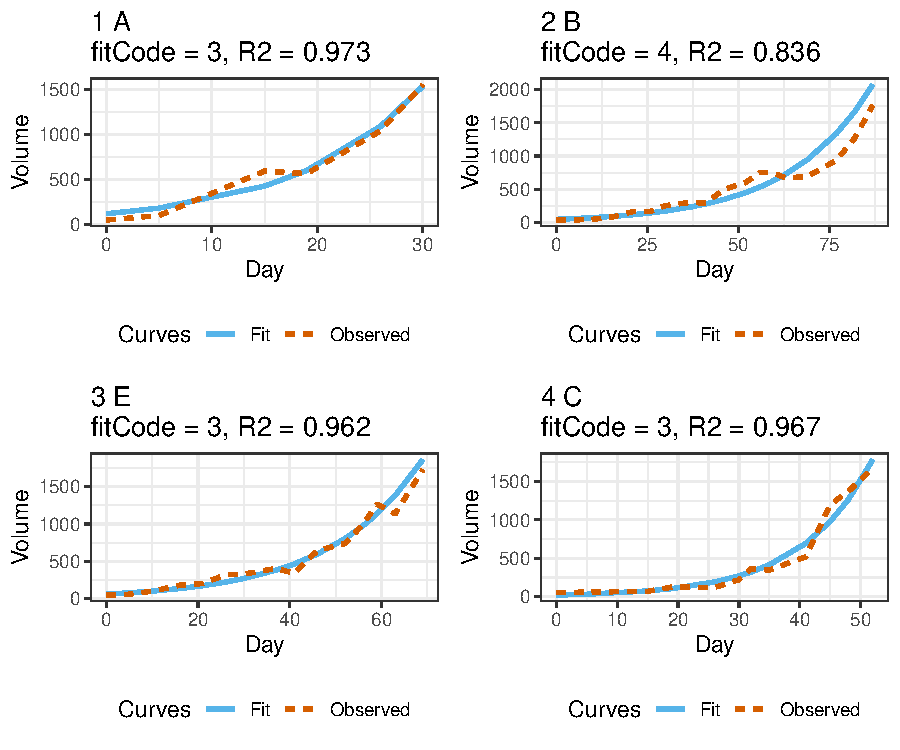
\includegraphics[width=0.9\textwidth]{img/mouse_fit.pdf}
\caption{Plot of \xt{mouse\_fit}, using \xt{data.table} syntax to subset to only the first four observations}
\label{fig:plot_fits}
\end{figure}

\subsection{Bootstrapping}

Once fits have been made, we are ready to begin estimating the group distributions and investigating temporal differences. This is done with the bootstrapping (and now permutation) function, \xt{bboot}. The number of options included in the \xt{bboot} function have expanded to include a new formula syntax for specifying the analysis of interest as well as to include options for permutation testing. A call to \xt{bboot} takes the following form

\begin{singlespace}
\begin{figure}[H]
\centering
\begin{BVerbatim}
bboot(formula, bdObj, B, alpha, permutation = TRUE, padj = "oleson", ...)
\end{BVerbatim}

\end{figure}
\end{singlespace}

The \xt{formula} argument is new to  \xt{bdots} and will be discussed in the next section. As for the remaining arguments, \xt{bdObj} is simply the object returned from \xt{bfit} that we wish to investigate, and \xt{B} serves the dual role of indicating the number of bootstraps/permutations we wish to perform. \xt{alpha} is the rate at which we wish to control the FWER. \xt{permutation} and \xt{padj} work in contrast to one another: when \xt{permutation = TRUE} (the default?), the argument to \xt{padj} is ignored. Otherwise, \xt{padj} indicates the method to be used in adjusting the nominal \xt{alpha} to control the FWER. By default, \xt{padj = "oleson"}. Finally, as previously mentioned, there is no longer a need to specify if the groups are paired, and \xt{bboot} determines this automatically based on the subject identifiers in each of the groups.


\paragraph{Formula}

As the \xt{bfit} function is now able to create fits for an arbitrary number of groups at once, we rely on a formula syntax in \xt{bboot} to specify precisely which groups differences we wish to compare. Let \xt{y} designate the outcome variable indicated in the \xt{bfit} function and let \xt{group} be one of the group column names to which our functions were fit. Further, let \xt{val1} and \xt{val2} be two values within the \xt{group} column. The general syntax for the \xt{bboot} function takes the following form:

\begin{singlespace}
\begin{figure}[H]
\centering
\begin{BVerbatim}
y ~ group(val1, val2)
\end{BVerbatim}
%\caption{Illustration of Mouse data}
\end{figure}
\end{singlespace}

Note that this is an \textit{expression} in R and is written without quotation marks. To give a more concrete example, suppose we wished to compare the difference in tumor growth curves for A and B from the \xt{Treatment} column in our mouse data (Figure~\ref{fig:mouse_head}). We would do so with the following syntax:

\begin{singlespace}
\begin{figure}[H]
\centering
\begin{BVerbatim}
Volume ~ Treatment(A, B)
\end{BVerbatim}
%\caption{Illustration of Mouse data}
\end{figure}
\end{singlespace}

There are two special cases to consider when writing this syntax. The first is the situation that arises in the case of multiple or nested groups, the second when a difference of difference analysis is conducted. Details on both of these cases are handled in the appendix. 



\paragraph{Summary and Analysis}

[what gets a paragraph, what gets a subsubsection?  compare this with \textit{\textbf{subsection}} for fitting]

Let's begin first by running \xt{bboot} using bootstrapping to compare the difference in tumor growth between treatment groups A and E in our mouse data using permutations to test for regions of significant difference. 

\begin{singlespace}
\begin{figure}[H]
\centering
\begin{BVerbatim}
mouse_boot <- bboot(Volume ~ Treatment(A, E), bdObj = mouse_fit, permutation = TRUE)
\end{BVerbatim}
%\caption{Illustration of Mouse data}
\end{figure}
\end{singlespace}


This returns an object of class \xt{bdotsBootObj}. A summary method is included to display relevant information:

\begin{singlespace}
\begin{figure}[H]
\centering
\begin{BVerbatim}
> summary(mouse_boot)

bdotsBoot Summary

Curve Type: expCurve 
Formula: Volume ~ x0 * exp(Day * k) 
Time Range: (0, 59) [21 points]

Difference of difference: FALSE 
Paired t-test: FALSE 
Difference: Treatment 

FWER adjust method: Permutation 
Alpha: 0.05 
Significant Intervals:
     [,1] [,2]
[1,]   15   32
\end{BVerbatim}
%\caption{Illustration of Mouse data}
\end{figure}
\end{singlespace}

There are a few components of the summary that are worth identifying when reporting the results. In particular, note the time range provided, an indicator of if the test was paired, and which groups were being considered \cn{(noticing now it only has \xt{Treatment}, not \xt{A} or \xt{E})}. The last section of the summary indicates the testing method used, an adjusted \xt{alphastar} if \xt{permutation = FALSE}, and a matrix of regions identified as being significantly different. This matrix is \xt{NULL} is no differences were identified at the specified alpha; otherwise there is one row included for each disjointed region of significant difference.

In addition to the provided summary output, a \xt{plot} method is available, with a list of additional options included in \xt{help(plot.bdotsBootObj)}.

\begin{figure}[H]
\centering
\begin{BVerbatim}
plot(mouse_boot)
\end{BVerbatim}

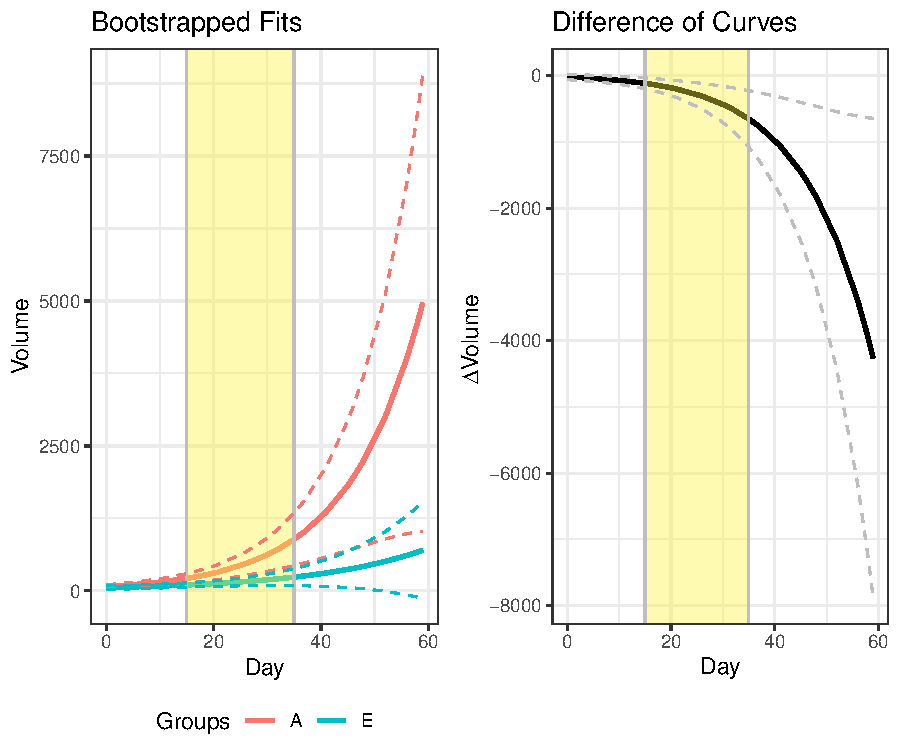
\includegraphics{img/mouse_boot_plot.pdf}
\caption{Bootstrapped distributions with regions of significant difference determined via permutation testing \cn{There are some obvious issues with time for non-homogenous samples, namely, what do we use for bootstrapping? It will be quick fix, whatever we decide, but I don't think ``union of all observed times" is going to work. Here, I artificially cut it back to only 0-60}}
\end{figure}
%
%Depending on user needs, these plots can be recreated both without confidence bands or without the additional difference curve
%
%\begin{figure}[H]
%\centering
%\begin{BVerbatim}
%plot(mouse_boot, ciBands = FALSE, plotDiffs = FALSE)
%
%\end{BVerbatim}
%
%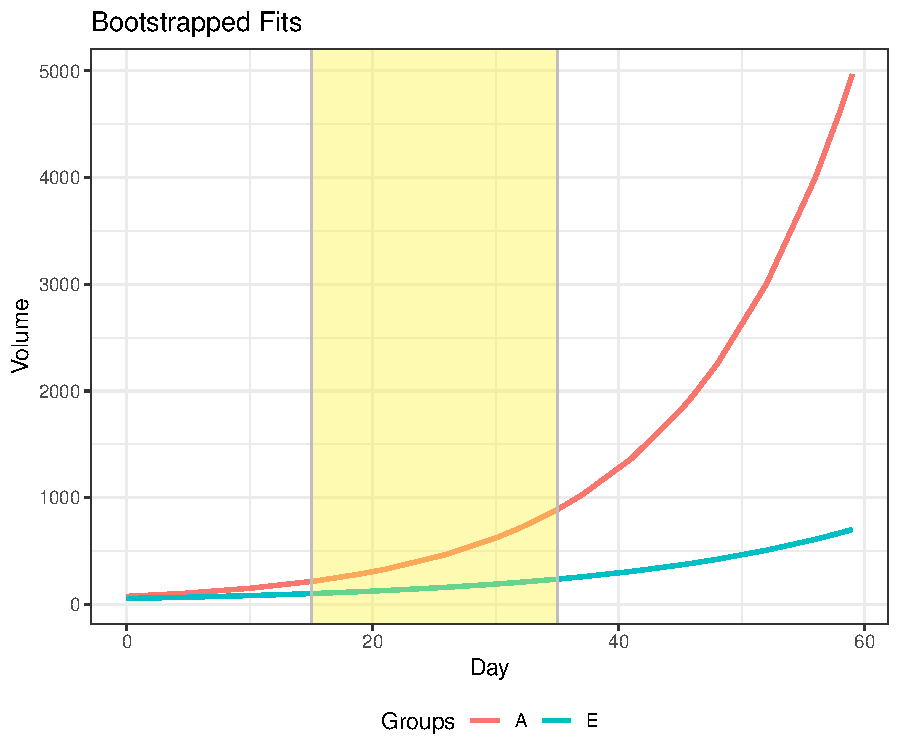
\includegraphics{img/mouse_boot_plot_extra.pdf}
%\caption{I think I'm going to actually not include this}
%\end{figure}


\section{Ancillary Functions}

Include here are a number of different function in \xt{bdots} facilitating  analysis but are otherwise not strictly necessary

\subsection{Refitting}

There are sometimes situations in which the fitted function returned by \texttt{bfit} is a poor fit. The nonlinear curve fitting algorithm used by \xt{nlme::gnls} in \xt{bfit} can be sensitive to starting parameters. Sensible starting parameters are computed from the observed data as part of the curve fitting functions (i.e., within the \xt{logistic()} function), though these can often be improved upon.


The quality of the fit can be evidenced by the \texttt{fitCode} or via a visual inspection of the fitted functions against the observations for each subject.  When this occurs, there are several options available to the user, all of which are provided through the function \texttt{brefit} (previously \texttt{bdotsRefit}). \texttt{brefit} takes the following arguments:

\begin{singlespace}
\begin{figure}[H]
\centering
\begin{BVerbatim}
brefit(bdObj, fitCode = 1L, subset = NULL, quickRefit = FALSE, paramDT = NULL)
\end{BVerbatim}
%\caption{Illustration of Mouse data}
\end{figure}
\end{singlespace}

The first of these arguments outside of the \xt{bdObj} is \xt{fitCode}, indicating the minimum fit code to be included in the refitting process. As discussed in Section~\ref{sec:fitcode}, this can be sub-optimal. To add flexibility to which subjects are fit there is now the \xt{subset} argument taking either a logical expression or collection of indices that would be used to subset an object of class \xt{data.table} (am I explaining this clearly?) or a numeric vector with indices that the user wishes to refit.

To assist with the refitting process is the argument \xt{quickRefit}. When set to \xt{TRUE}, \xt{brefit} will take the average coefficients of accepted fits within a group and use those as new starting parameters for poor fits. The new fits will be retained if they have a larger $R^2$ value by default. When set to \xt{quickRefit = FALSE}, the user will be guided through a set of prompts to refit each of the curves manually. 

Finally, the \texttt{paramDT} argument allows for a \xt{data.table} with columns for subject, group identifiers, and parameters to be passed in as a new set of starting parameters. This \xt{data.table} requires the same format as that returned by \xt{bdots::coefWriteout}. The use of this functionality is covered in more detail in the \xt{bdots} vignettes and is a useful way for reproducing a \xt{bdotsObj} from a plain text file. 

When \texttt{quickRefit = FALSE}, the user is put through a series of prompts along with a series of diagnostics for each of the subjects to be refit. Here, for example, is the option to refit subject 11 from the mouse data:


\begin{singlespace}
\begin{figure}[H]
\centering
\begin{BVerbatim}
Subject: 11
R2: 0.837
AR1: FALSE
rho: 0.9
fitCode: 4

 Model Parameters:
       x0         k 
53.186497  0.051749 

Actions:
1) Keep original fit
2) Jitter parameters
3) Adjust starting parameters manually
4) Remove AR1 assumption
5) See original fit metrics
6) Delete subject
99) Save and exit refitter
Choose (1-6):
\end{BVerbatim}
%\caption{Illustration of Mouse data}
\end{figure}
\end{singlespace}

There are a number of options provided in this list. The first, of course, keeps the original fit of the presented subject and moves on to the next subject in the list. The second option takes the values of the fitted parameter and ``jitters" them, changing each of the values by a prespecified magnitude. Given the sensitivity of \xt{nlme::gnls} to starting parameters, this is sometimes enough for the fitter to converge on a better fit for the observed data. Alternatively, the third option gives the user the ability to select the starting parameters manually. The third option gives the user the ability to attempting refitting the observed data without an AR(1) error assumption, though this is only relevant if such an assumption exists. Option (5) reprints summary information and the final option allows the user to delete the subject all together.

When any attempt to refit the observed under new conditions is presented (options (2)-(4)), a plot is rendered comparing the original fit side-by-side with the new alternative, Figure~\ref{fig:refit_plot}.

\begin{figure}[H]
\centering
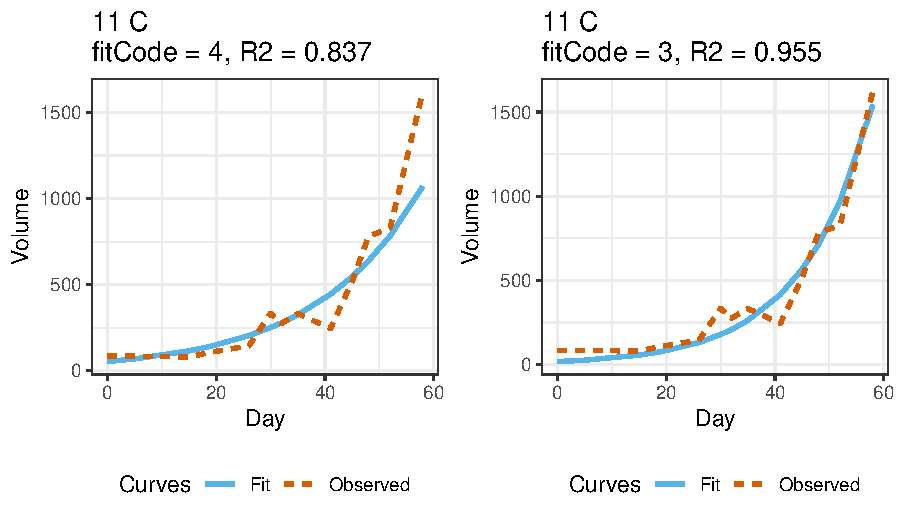
\includegraphics{img/mouse_refit_plot.pdf}
% new pars x0=50, k = 0.06
\caption{before and after refit}
\label{fig:refit_plot}
\end{figure}

As the menu item suggests, users have the ability to end the manually refitting process early and save where they had left off. To retain previously refit items and start again at a later time, pass the first refitted object back into the refitter as such:

\begin{singlespace}
\begin{figure}[H]
\centering
\begin{BVerbatim}
refit <- brefit(fit, ...)
refit <- brefit(refit, ...) # pass in the refitted object
\end{BVerbatim}
%\caption{Illustration of Mouse data}
\end{figure}
\end{singlespace}



A final note should be said regarding the option to delete a subject. As \xt{bdots} now automatically determines if subjects are paired based on subject identifiers (necessary for  calculations in significance testing), it is critical that if a subject has a poor fit in one group and must be removed that he or she is also removed from all additional groups in order to retain paired status. This can be overwritten with a final prompt in the \texttt{brefit} function before they are removed. The removal of subjects can also be done with the ancillary function, \texttt{bdRemove}, useful for removing subjects without undergoing the entire refitting process. See \xt{help(bdRemove)} for details.


\subsection{Correlations}

There are sometimes cases in which we are interested in determining the correlation of a fixed attribute with group outcome responses across time . This can be done with the \texttt{bcorr} function (previously \texttt{bdotsCorr}), which takes as an argument an object of class \texttt{bdotsObj} as well as a character vector representing a column from the original dataset used in \texttt{bfit}

\begin{center}
\xt{bcorr(fit, "value", ciBands, method = "pearson")} 
\end{center}

Need to elaborate here with example

\subsection{$\alpha$ Adjustment}

There may also be situations in which users wish to make an adjustment to autorcorrelated test statistics using the modified Bonferonni adjustment provided in \cite{oleson2017detecting}, though in a different context than what is done in \xt{bdots}. To facilitate this, we introduce an extension to the \texttt{p.adjust} function, \texttt{p\_adjust}, identical to \texttt{p.adjust} except that it accepts method \texttt{"oleson"} and takes additional arguments \texttt{rho}, and \texttt{df}. \texttt{rho} determines the autocorrelation estimate for the oleson adjustment while \texttt{df} returns the degrees of freedom used to compute the original vector of t-statistics. If an estimate of \texttt{rho} isn't available, one can be computed on a vector of t-statistics using the \texttt{ar1Solver} function in \xt{bdots}:

%\begin{center}
%\texttt{t <- diffinv(rnorm(100))} \\
%\texttt{rho <- ar1Solver(t)} \\
%\texttt{unadj\_p <- pt(t, df = 10)} \\
%\texttt{adj\_p <- p\_adjust(unadj\_p, method = "oleson", df = 10, rho = rho, alpha = 0.05)}
%\end{center}


\begin{singlespace}
\begin{figure}[H]
\centering
\begin{BVerbatim}
t       <- diffinv(rnorm(5))
rho     <- ar1Solver(t)
unadj_p <- pt(t, df = 10)
adj_p   <- p_adjust(unadj_p, method = "oleson", 
                    df = 10, rho = rho, alpha = 0.05)
\end{BVerbatim}
%\caption{Illustration of Mouse data}
\end{figure}
\end{singlespace}

The \xt{p\_adjust} function returns both adjusted p-values, which can be compared against the specified alpha (in this case, $0.05$) along with an estimate of alphastar, a nominal alpha at which one can compare the original p-values:

\begin{singlespace}
\begin{figure}[H]
\centering
\begin{BVerbatim}
> unadjp
[1] 0.5000000 0.0849965 0.0381715 0.1601033 0.0247453 0.0013016
> adjp
[1] 0.9201915 0.1564261 0.0702501 0.2946514 0.0455408 0.0023954
attr(,"alphastar")
[1] 0.027168
\end{BVerbatim}
%\caption{Illustration of Mouse data}
\end{figure}
\end{singlespace}

Here, for example, we see that the last two positions of \xt{unadjp} have values less than \xt{alphastar}, identifying them as significant; alternatively, we see these same two indices in \xt{adjp} significant when compared to \xt{alpha = 0.05}

\section{Discussion}


The original implementation of \xt{bdots} set out to address a narrow set of problems. Previous solutions beget new opportunities, however, and it is in this space that the second iteration of \xt{bdots} has sought to expand. Since then, the interface between user and application has been significantly revamped, creating a intuitive, reproducible workflow that is able to quickly and simply address a broader range of problems. The underlying methodology has also been improved and expanded upon, offering better control of the family-wise error rate.

While significant improvements have been made, there is room for further expansion. The most obvious of these is the need to include support for non-parametric functions, the utility of which cannot be overstated. Not only would this alleviate the need for the researcher to specify in advance a functional form for the data, it would implicitly accommodate more heterogeneity of functional forms within a group. Along with this, the current implementation is also limited in the quality-of-fit statistics used in the fitting steps to assess performance. $R^2$ and the presence of autocorrelation are relevant to only a subset of the types of data that can be fit, and allowing users more flexibility in specifying this metric is an active goal for future work. In all, future directions of this package will be primarily focused on user interface, non-parametric functions, and greater flexibility in defining metrics for fitted objects.



\section*{Appendix}

This section currently commented out. Involves instructions for fitting difference of difference and nested groups. Also may possibly include custom curve fitting.

%
%
%
%\section*{Appendix X} \\
%
%We will illustrate use of the updated \xt{bdots} package with a worked example, using an artificial dataset to help detail some of the newer aspects of the package. The dataset will consist of outcomes for a collection of vehicles, consisting of eight distinct groups. These groups will be nested in order of vehicle origin (foreign or domesetic), vehicle class (car or truck), and vehicle color (red or blue). Further, vehicles of different color but within the same origin and class groups will be considered paired observations. A table detailing the relationship of the groups is shown here:
%
%
%
%The outcome here is simply \xt{y} due to a lack of creativity, but the functional form assumed (and used in data generation) follows the four parameter logistic, 
%
%\begin{equation}
%f_{\theta}(t) = b + \frac{p-b}{1 + \exp \left( \frac{4s}{p-b} (x-t) \right)},
%\end{equation}
%where $b$, $p$, $s$, and $x$ represent the baseline, peak, slope, and crossover points, respectively
%
%
%
%The formula argument serves two functions in \xt{bboot}: first, it specifies the collection of curves we wish to investigate the difference between, and second, it determines if we are interested in directly comparing the differences or the difference of differences between curves. 
%
%To begin, let's reintroduce the structure of the groups we have in our dataset. Recall that we have foreign and domestic cars and trucks, and each of these vehicles comes in red and blue. Recall also that the different colors of each vehicle are considered paired observations.
%
%\begin{table}
%\centering
%\def\arraystretch{1.5}
%\begin{tabular}{|p{0.9in}|p{0.9in}|p{0.9in}|} \hline 
%\rowcolor{lightgray} \multicolumn{1}{|c|}{Origin} & \multicolumn{1}{c|}{Class} & \multicolumn{1}{c|}{Color}\\
%\hline
%\multirow{4}{*}{foreign} & \multirow{2}{*}{car} & red \\
%\hhline{~~-}
%& & blue \\
%\hhline{~--}
%& \multirow{2}{*}{truck} & red \\
%\hhline{~~-}
%& & blue \\
%\hline
%\multirow{4}{*}{domestic} & \multirow{2}{*}{car} & red \\
%\hhline{~~-}
%& & blue \\
%\hhline{~--}
%& \multirow{2}{*}{truck} & red \\
%\hhline{~~-}
%& & blue \\
%\hline
%\end{tabular}
%\caption{table of stuff}
%\label{tab:group_table}
%\end{table}
%
%
%Beginning with a simple case, suppose we want to investigate the difference in outcome between foreign and domestic vehicles. Notionally, we would write
%
%\begin{center}
%\tt y $\sim$ Origin(foreign, domestic).
%\end{center}
%
%
%Note that this involves the grouping variable, \xt{Origin}, with the two values we are interested in comparing, \xt{domestic} and \xt{foreign}. With this specification, the distribution of functions considered in \xt{domestic} include all red and blue domestic cars and trucks.
%
%
%If we wanted to limit our investigation to only foreign and domestic \textit{trucks}, we would do this by including an extra term specifying the group and the desired value. In this case, 
%
%\begin{center}
%\tt y $\sim$ Origin(foreign, domestic) + Class(truck).
%\end{center}
%To compare only foreign and domestic \textit{red} trucks, we would add an additional term for color:
%
%\begin{center}
%\tt y $\sim$ Origin(foreign, domestic) + Class(truck) + Color(red).
%\end{center}
%
%There are also instances in which we might be considered in the interaction of two groups. Although there is no native way to handle interactions in \xt{bdots}, this can be done indirectly through the difference of differences (McMurray et al 2019, though truthfully I still don't understand why). To illustrate, suppose we are interested in understanding how the color of the vehicle differentially impacts outcome based on the vehicle class. In such a case, we might look at the difference in outcome between red cars and red trucks, and then again the difference between blue cars and blue trucks. Any difference between these two differences would give information regarding the differential impact of color between each of the two classes. This is done in \xt{bdots} using the \xt{diffs} synatx in the formula:
%
%%\textbf{FOUND SOURCE FOR THIS:} \textit{McMurray, Klein-Packard, Tomblin 2019, real time mechanics..pg 7}
%
%\begin{center}
%\tt diffs(y, Class(car, truck)) $\sim$ Color(red, blue)
%\end{center}
%
%Here, the \textit{outcome} that we are considering is the difference between vehicle classes, with the outcome of interest being color. This is helpful in remembering which term goes on the LHS of the formula. 
%
%Similar as to the case before, if we wanted to limit this difference of differences investigation to only include domestic vehicles, we can do so by including an additional term:
%
%\begin{center}
%\tt diffs(y, Class(car, truck)) $\sim$ Color(red, blue) + Origin(domestic).
%\end{center}
%
%The formula syntax was originally contrived to make comparisons within groups or within nested groups. Conceivably, however, one could be interested in making the comparison between domestic red trucks and foreign blue cars. Doing so requires a bit of a work around. Examples detailing how one might go about doing this are included in appendix B. 
%
%\section*{Appendix B - Fitting non-nested groups}
%
%(currently just copy pasted from the body of document, not edited so no need to really review)
%
%First, there would be some function of sorts, something like \xt{makeUniqueGroups} which would create a new group column with each permutation of previous groups being given a unique identifier. Doing this on the vehicle example would look something like \xt{fit <- makeuniquewhatever} resulting in the following grouping structure (for example) (and maybe you could specify group name and values who knows, kinda like factor this is just a working thought example)
%
%\begin{center}
%
%\begin{tabular}{|p{0.9in}|p{0.9in}|p{0.9in}|p{0.5in}|} \hline 
%\rowcolor{lightgray} \multicolumn{1}{|c|}{Origin} & \multicolumn{1}{c|}{Class} & \multicolumn{1}{c|}{Color} & \multicolumn{1}{c|}{bgroup}\\
%\hline
%\multirow{4}{*}{foreign} & \multirow{2}{*}{car} & red & A\\
%\hhline{~~--}
%& & blue & B \\
%\hhline{~---}
%& \multirow{2}{*}{truck} & red & C\\
%\hhline{~~--}
%& & blue & D\\
%\hline
%\multirow{4}{*}{domestic} & \multirow{2}{*}{car} & red & E \\
%\hhline{~~--}
%& & blue & F\\
%\hhline{~---}
%& \multirow{2}{*}{truck} & red & G\\
%\hhline{~~--}
%& & blue & H\\
%\hline
%\end{tabular}
%\end{center}
%
%To then investigate differences in outcome between a foreign red car and a domestic blue truck would simply then be
%
%\begin{center}
%\tt y $\sim$ bgroup(A, H)
%\end{center}
%
%yeah not like sexy or anything but whatever it would work.
%
%


\newpage

\Chapter{look onset method}
\section{Introduction}


Spoken words create analog signals that are processed by the brain in real time. That is, as spoken word unfolds, a collection of candidate words are considered until the target word is recognized \citep{MarslenWilson1987}. The degree to which a particular candidate word is being considered is known as activation. An important part of this process involves not only correctly identifying the word but also eliminating competitors. For example, we might consider a discrete unfolding of the word ``elephant" as ``el-e-phant". At the onset of ``el", a listener may activate a cohort of potential resolutions such as ``elephant", ``electricity", or ``elder", all of which may be considered competitors. With the subsequent ``el-e", words consistent with the received signal, such as ``elephant" and ``electricity" remain active competitors, while incompatible words, such as ``elder", are eliminated. Such is a rough description of this process, continuing until the ambiguity is resolved and a single word remains.


Our interest is in measuring the degree of activation of a target, relative to competitors. Activation, however, is not measured directly, and we instead rely on what can be observed with physiological behavior. Although there are a number of relevant indices of lexical activation \citep{Spivey2005}, we concern ourselves here with eye tracking data collected in the context of the Visual World Paradigm (VWP) \cite{tanenhaus1995integration}, an experimental model in which a participant's eye movements are tracked as they respond to spoken language. Recently, however, researchers have begun to reexamine some of the underlying assumptions associated with the VWP, calling into question the validity or interpretation of current methods (\cite{Magnuson2019}, \cite{mcmurray2022m}). We present here a brief history of word recognition in the context of the VWP, along with an examination of contemporary concerns. In response, we then propose a new generative model for understanding eye mechanics, accompanied by an alternative method for relating eye-tracking data to lexical activation. We follow this with a series of simulations, both in the context of recovering the trajectory of eye mechanics for individual subjects, as well as for identifying differences in trajectories between groups of individuals. Finally, we demonstrate the performance of our model with an application to data collected in prior studies. 


\cn{these next sections``paragraphs" are a little short but i think that's ok}

\paragraph{Visual World Paradigm} The Visual World Paradigm (VWP) was first introduced in 1995, making the initial link between the mental processes associated with language comprehension and eye movements \citep{tanenhaus1995integration}. A typical experiment in the VWP involves situating a subject in front of a ``visual world", commonly a computer screen today, and asking them to identify and select an object corresponding to a spoken word. The initiation of eye movements and subsequent fixations are recorded as this process unfolds, with the location of the participants' eyes serving as a proxy for which words or images are being considered. This association was first demonstrated by comparing how the mean time to initiate an eye movement to the correct object was mediated by the presence of phonological competitors (``candy" and ``candle", sharing auditory signal at word onset) and situations containing syntactic ambiguity (``Put the apple on the towel in the box" and ``Put the apple \textit{that's} on the towel in the box" in ambiguous scenarios with one or more apples). It is by comparing the trajectory of these mechanics across trials in the presence of auditory or semantic competitors that researchers have used the VWP in their investigation of spoken word recognition. For a review, see \citet{Huettig2011}, \citet{salverda2017visual}.




\paragraph{Proportion of fixation} The interactive activation model of word recognition was first introduced in \citet{McClelland1981}, positing that word recognition takes place in a system with multiple interacting hierarchies of processing, including those made up of features, phonemes, and words. This model was later instantiated as a computer model known as TRACE \citep{elman1985speech}. Briefly, TRACE is structured as a hierarchical network model, in which input is fed into the system (typically as a string of phonemes), with potential resolutions (here, words) being represented as nodes. The TRACE model processes this input \textit{over time} and in parallel, with activation incrementally cascading from features (voicing, aspiration, etc.,) to phonemes to words. Multiple words can be activated at once, graded by consistency of the word with the received signal. Finally, the TRACE model exhibits competition, whereby the activation of a particular word functions to inhibit its competitors. This entire process continues as input is received until a single word is most active. An example of this is demonstrated in Figure~\ref{fig:trace_plot} using the current implementation of TRACE, jTRACE \citep{Strauss2007}, in which the word ``party" was provided as input. This figure shows the activation of the target word, along with a number of competitors.

\begin{figure}[H]
\centering
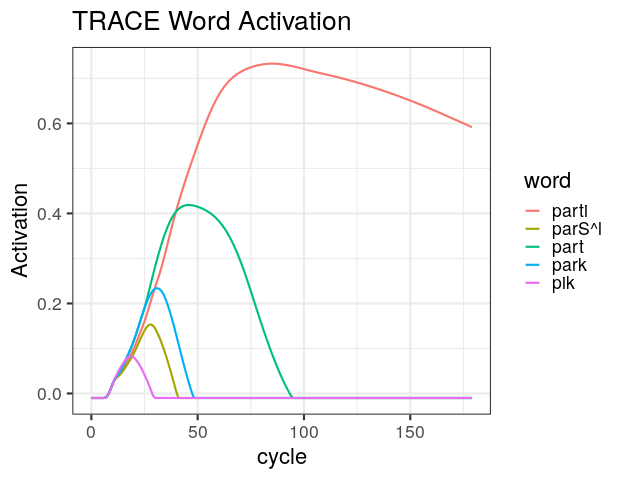
\includegraphics[scale=1]{trace_plot}
\caption{TRACE activation of the word ``party", with competitors}
\label{fig:trace_plot}
\end{figure}



It was against simulated TRACE data that \citet{allopenna1998tracking} found a tractable way of analyzing eye-tracking data collected in the VWP.  By coding the period of a fixation as a 0 or 1 for each referent and taking the average of fixations towards a referent at each time point, Allopenna was able to create a ``fixation proportion" curve that largely reflected the shape and competitive dynamics of word activation suggested by TRACE, both for the target object, as well as competitors. This also provided an empirical grounding for an explicit linking hypothesis, relating lexical activation to eye mechanics  (emphasis added):

\begin{quote}
We made the general assumption that the probability of initiating an eye movement to fixate on a target object $o$ at time $t$ is a direct function of the probability that $o$ is the target given the speech input and where the probability of fixating $o$ is determined by the activation level of its lexical entry relative to the activation of other potential targets. [...] Note that this hypothesis does \emph{not} require stronger and less defensible assumptions about the relationship between eye  movements and attention. For example, we are not committed to the assumption that scan patterns in and of themselves reveal underlying cognitive processes. \citep{allopenna1998tracking}
\end{quote}

The utility in this linking hypothesis comes from its simplicity, asserting only that the probability of fixating an object increases as the likelihood it has been referred to increases. \cn{said increases twice here}. This is in contrast to a number of more involved linking hypotheses presented in \citep{Magnuson2019}.


\paragraph{Parametric Methods and Individual Curves} While many studies have addressed qualitative aspects of word recognition such as feedback \citep{Magnuson2003}, or priming \citep{luce1998delayed}, few had offered consideration to individual differences in activation. A first attempt was provided by \citet{Mirman2008} using mixed effects models to capture subject-specific effects by fitting observed data to polynomial functions in time. While this addressed the problem of capturing individual differences, it was burdened by the fact that polynomials are often a poor fit for VWP data, often requiring a high degree to be appropriately fit, resulting in potentially poor asymptotic behavior. Further, polynomial coefficients are often unable to be intuitively mapped onto clinically relevant properties of the functions they are intended to emulate. This was the position taken by \citet{mcmurray2010individual}, who first introduced non-linear functions to the observed data, equipped with readily interpretable and clinically relevant properties. This includes the four parameter logistic function provided in Equation~\ref{eq:logistic} as well as the double Gaussian function given in Equation~\ref{eq:dg}. Outside of serving to address psycholinguistic concerns relating to individual differences in word recognition, this advancement has been critical in shaping current statistical models used in the context of the VWP. The specification of subject-specific parameters itself implies a distribution of parameters within an experimental group, serving as an impetus for investigating group differences in word activation through the use of bootstrapped differences in time series \citep{oleson2017detecting} and the subsequent development of the \xt{bdots} software in R for analyzing such differences \citep{seedorff2018bdots}.



\begin{figure}[h]
\centering
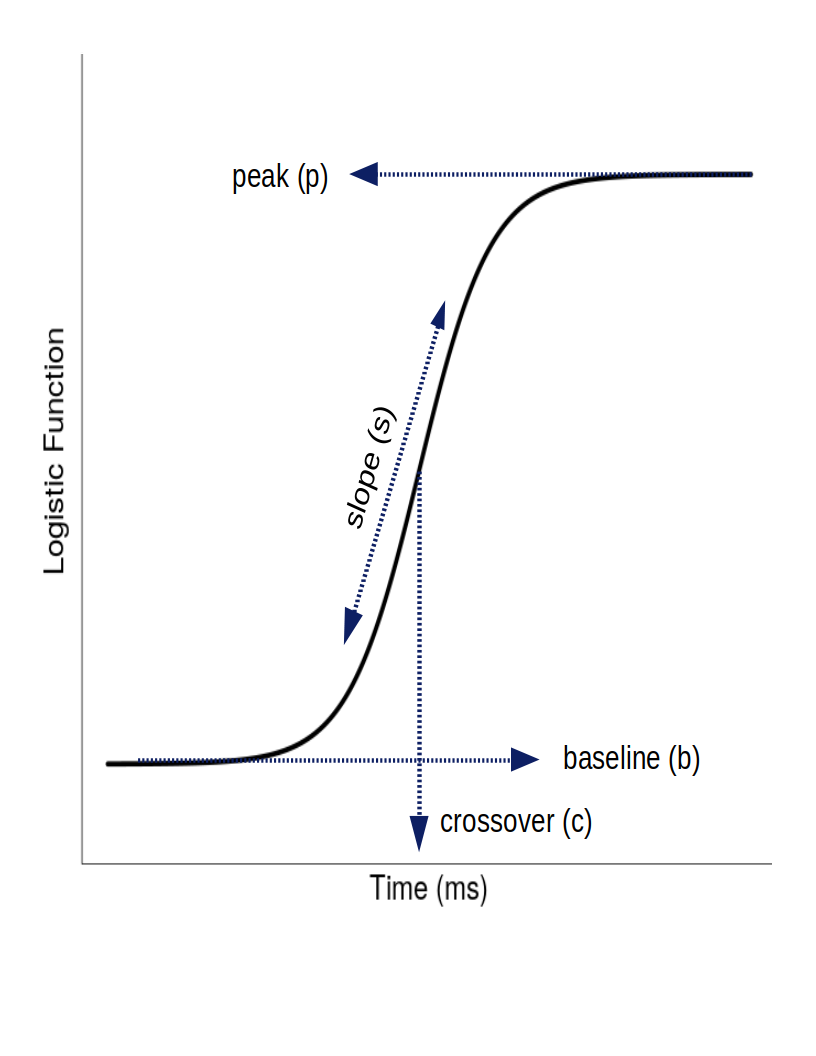
\includegraphics[scale=0.4]{logistic_label.png}
\caption{An illustration of the four-parameter logistic (Equation~\ref{eq:logistic}) and its associated parameters, introduced as a parametric function for fixations to target objects}
\label{fig:logistic_definition}
\end{figure}

\cn{say a bit here to transition to next section?}


\section{Analysis with VWP Data}

We now shift focus to the physiological mechanics of eye movements in the context of the Visual World Paradigm, including a mathematical description of how these mechanics relate to the proportion of fixation method first introduced by \citet{allopenna1998tracking}.  




\subsection{Anatomy of Eye Mechanics}

While a number of experimental methods are used as real-time indices of lexical access \citep{Spivey2005}, we concern ourselves here with the use of eye tracking, given that ``eye movements to objects in the workspace are closely time-locked to referring expressions in the unfolding speech stream, providing a sensitive and nondistruptive measure of spoken language comprehension during continuous speech \citep{allopenna1998tracking}." This process in its entirety is made up of several interrelated components, including activation and the visual-motor system, oculomotor delay, and mechanics of eye movement itself. We briefly introduce each of these components in turn, while providing a visual summary in Figure \cn{make figure for this}

\begin{figure}[H]
\centering
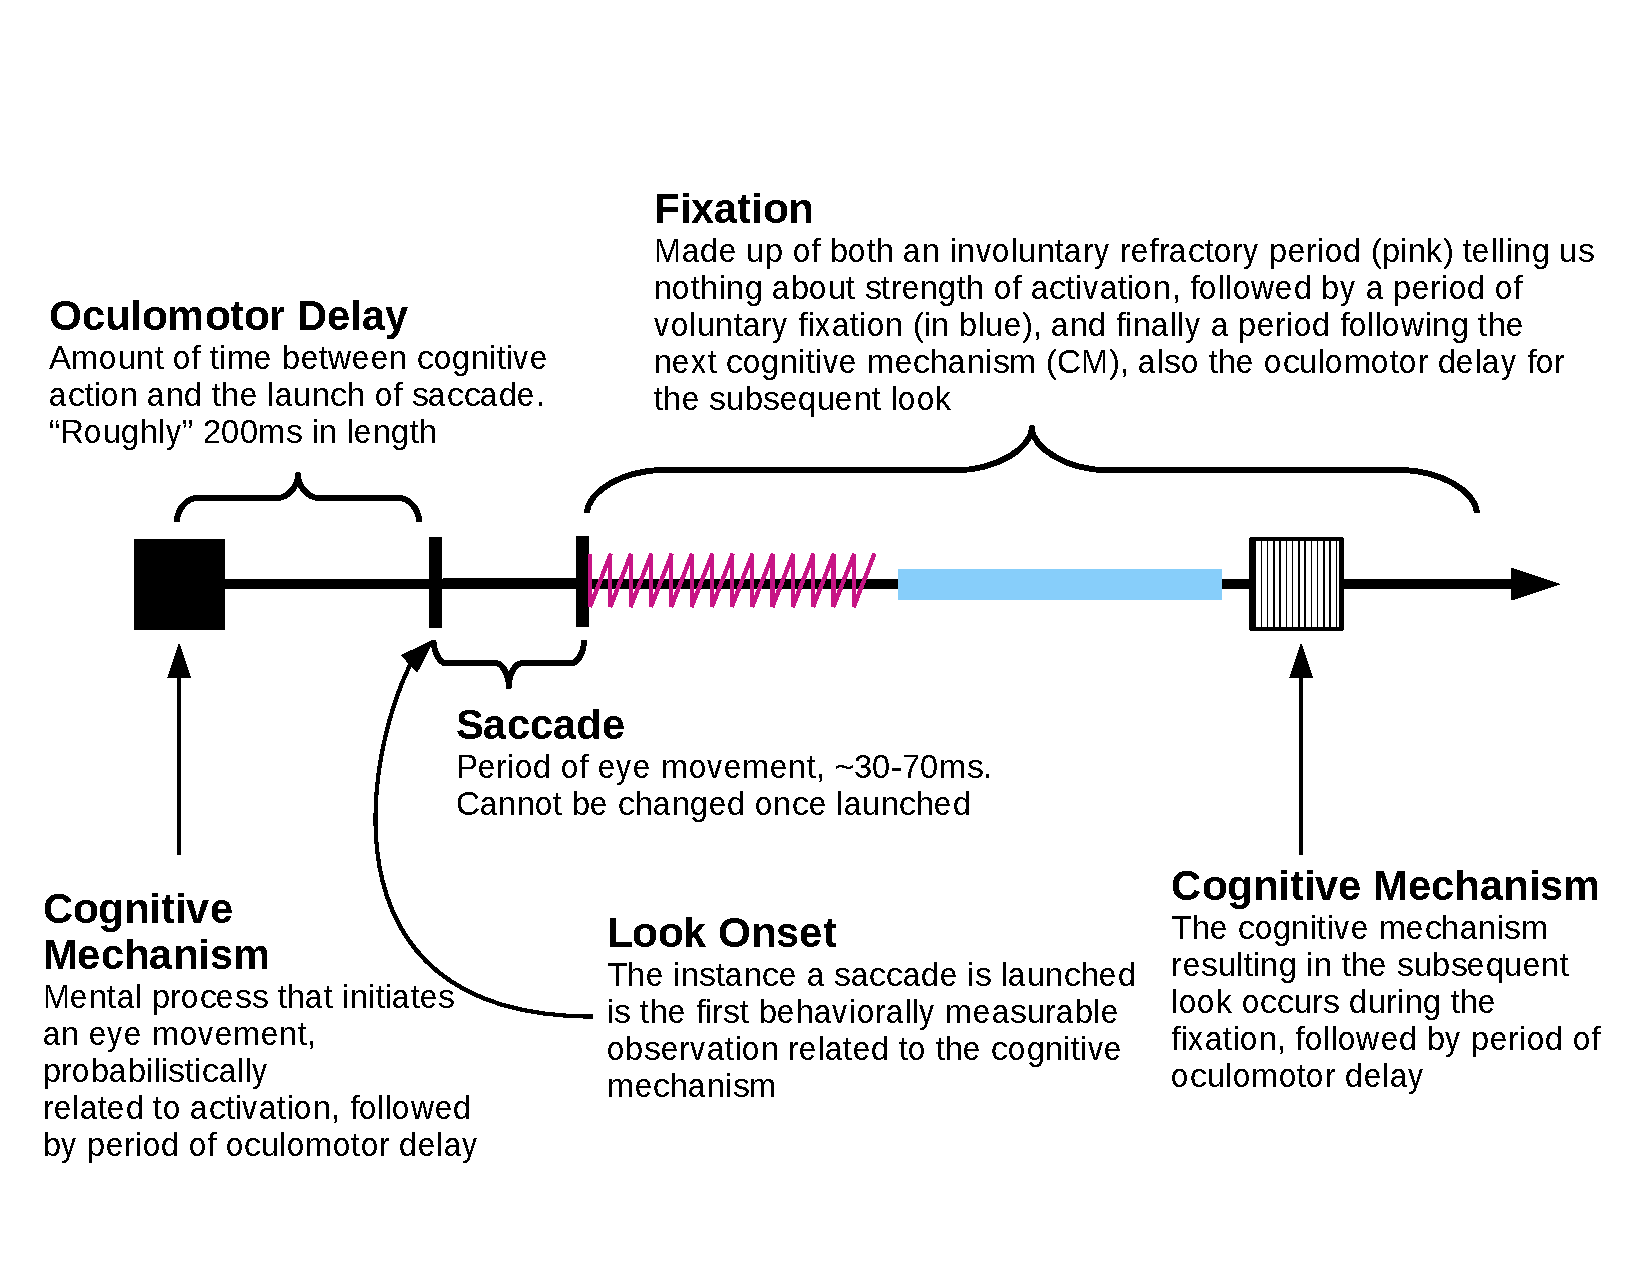
\includegraphics[scale=0.5]{what_is_a_look.pdf}
\caption{A visual depiction of the anatomy of a look} 
\label{fig:whats_in_a_look}
\end{figure}

\subsubsection{Saccades and Fixation}

Rather than acting in a continuous sweeping motion as our perceived vision might suggest, our eyes themselves move about in a series of short, ballistic movements, followed by brief periods of stagnation. These periods of movement and stagnation, respectively, are the saccades and fixations. 

Saccades are short, ballistic movements lasting between 20ms-60ms, during which time we are effectively blind. Once in motion, saccades are unable to change trajectory from their intended destination. Following this movement is a period known as a fixation, itself made up of a necessary refraction period (during which time the eye is incapable of movement) followed by a period of voluntary fixation which may include planning time for deciding the destination of the next eye movement; the duration of fixations are typically longer and more variable. It will be convenient to follow previous convention and consider a saccade followed by its adjacent fixation as a single concept called a ``look" \cite{mcmurray2002look}. We take particular care here to note that the beginning of a look, or ``look onset", starts the instance that a previous look ends or, said another way, the instant an eye movement is launched. 

The mechanical aspects of eye movements are not themselves what we are interested in. Rather, they serve as an index of the underlying cognitive process, lexical activation, which we discuss next..

\subsubsection{Activation and Visual-Motor system}

The concept of activation, as it relates to the discussion here, arises from the metaphor in which word perception is made up of a network made up of hierarchical levels (letter, phoneme, word, etc.,) acting as an interactive process unfolding in time \cite{McClelland1981}. Under this \textit{interactive activation model}, greater activation is associated with a greater excitatory action for a network node (specifically here, a word) resulting from consistency with the received auditory signal. The interactive activation model allows for both excitatory and inhibiting activations, resulting in the ``competing" activation curves between candidate resolutions as the auditory signal unfolds. A theoretical example of activation is given in Figure~\ref{fig:trace_plot}.

Eye movements themselves are not a direct read-out of activation, and instead are downstream of a much larger process that also involves the visual-motor system, including general stimulus processing and environment scanning \citep{Salthouse1980}. It is this peripheral system, in conjunction with lexical activation, that leads to the \textit{probabilistic} association of activation and fixations. Any proposed relation of each of these in detail to saccades and fixations is known as a \textit{linking hypothesis} tying the observed to the theoretical \citep{Magnuson2019}. 

For our purposes here, we take no stronger a position than acknowledging the interplay between these processes and acknowledging their culmination as a ``cognitive mechanism" (CM) that ultimately initiates the launching of a saccade, a mechanism itself that is probabilistically related to activation.



\subsubsection{Oculomotor Delay}

In between the cognitive mechanism that initiates the decision to launch an eye movement and the movement itself is a period known as oculomotor delay. It is typically estimated to take around 200ms to plan and launch an eye movement \cite{viviani1990time}, and this is usually accounted for by subtracting 200ms from any observed behavior. As oculomotor delay is only ``roughly" estimated to be around 200ms, we suggest that accounting for randomness will be critical in correctly recovering the the cognitive mechanism of interest or at very least in identifying possible sources of bias or error. 





\subsection{Proportion of Fixation Method}


We now consider how the aforementioned mechanics relate to the visual world paradigm. In a typical implementation of the Visual World Paradigm in an experiment, a participant is asked to complete a series of trials during each of which they are presented with a number of competing images on screen (typically four). A verbal cue is given, and the participants are asked to select the image corresponding to the spoken word. All the while, participants are wearing (generally) a head-mounted eye tracking system recording where on screen they were fixated. 

An individual trial of the VWP may be short, lasting anywhere from 1000ms to 2500ms before the correct image is selected. Prior to selecting the correct image, the participant's eyes scan the environment, considering images as potential candidates to the spoken word. As this process unfolds, a snapshot of the eye is taken at a series of discrete steps (typically every 4ms) indicating where on the screen the participant is fixated. A single trial of the VWP typically contains no more than four to eight total ``looks" before the correct image is clicked, resulting in a paucity of data in any given trial.

To be clear, eye trackers themselves only record $x$ and $y$ coordinates of the eye at any given time, and it is only after the fact that ``psychophysical" attributes are mapped onto the data (saccades, fixations, blinks, etc.,). We adopt the strategy of prior work in discussing eye tracking data in terms of their physiological mapping, as this will be crucial in constructing a physiologically relevant understanding of the problem at hand \cite{mcmurray2002look}.

\begin{figure}[H]
\centering
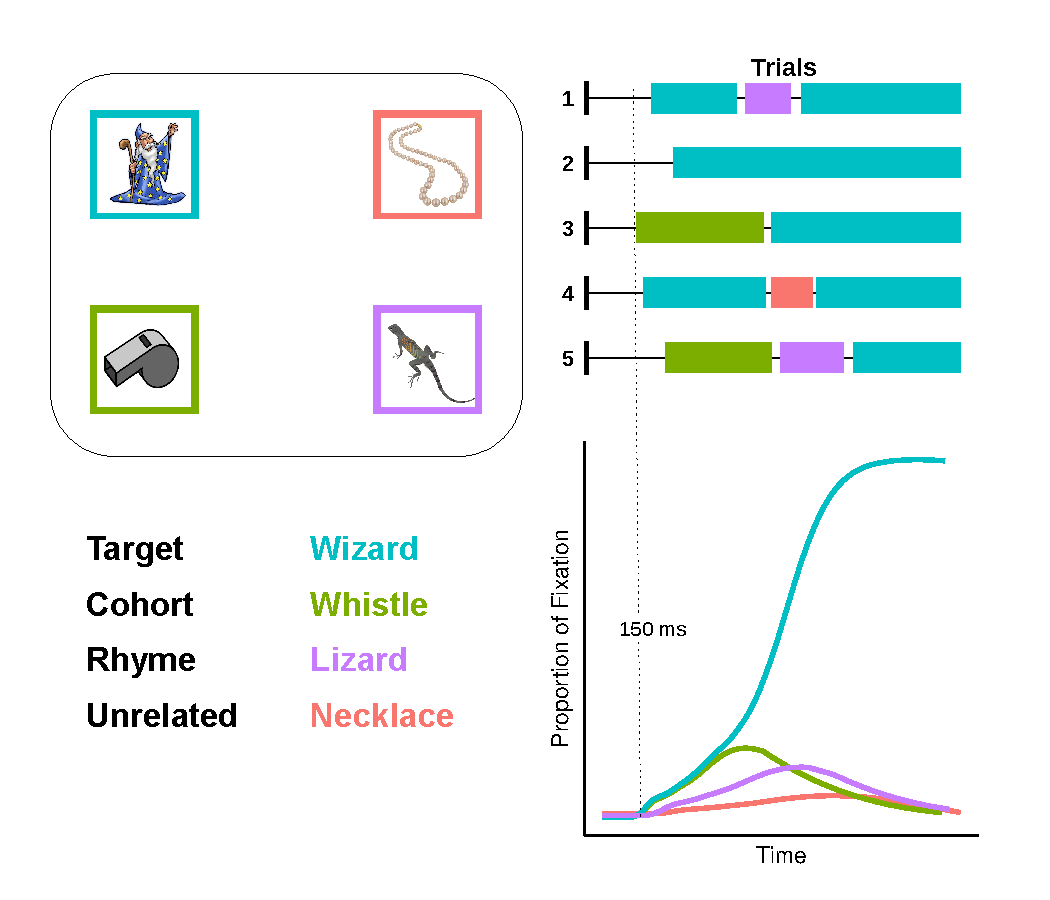
\includegraphics[scale=0.7]{collin_diagram_full.pdf}
\caption{Stole this from Bob (who apparently stole it from richard aslin), plan on making my own}
\label{fig:collin_diagram_full}
\end{figure}


To create a visual summary of this process aggregated over all of the trials, a la Allopena, a ``proportion of fixations" curve is created, aggregating at each discrete time point the average of indicators of whether or not a participant is fixated on a particular image. A resulting curve is created for each of the competing categories (target, cohort, rhyme, unrelated), creating an empirical estimate of the activation curve, $f(t|\theta)$. See Figure~\ref{fig:bob_diagram_full}. For any subject $i = 1, \dots, n$, across times $t = 0, \dots, T$ and trials $j = 1, \dots, J$, a construction  of this curves can be expressed as:


\begin{equation}\label{eq:sum_proportions}
y_{it} = \frac1J \sum_{j=1}^J z_{ijt}
\end{equation}
where $z_{ijt}$ is an indicator $\{0, 1\}$  towards a particular object in trial $j$ at time $t$. Following the contributions of \citet{mcmurray2010individual}, we model the empirical curve given in Equation~\ref{eq:sum_proportions} with a parametric function $f(t|\theta)$, identifying subject-specific parameters $\theta_i$ which describe clinically relevant attributes of the curve, 

\begin{equation}\label{eq:empir_to_activation}
f(t | \theta_i) \equiv y_{it}.
\end{equation}

The recovery of subject-specific parameters occurs by subjecting the observed data to a simple loss function, 

\begin{equation}\label{eq:prop_loss}
\hat{\theta} = \argmin_{\theta} \mathcal{L}(f_{\theta}, y).
\end{equation}

As mentioned previously, fixations to the Target in a VWP experiment are often modeled with the four parameter logistic function (Figure~\ref{fig:logistic_definition}), 

\begin{equation} \label{eq:logistic}
f(t|\theta) = \frac{p-b}{1 + \exp \left(\frac{4s}{\text{p}-b} (x - t) \right)} + b.
\end{equation}

Similarly, a six parameter asymmetric Gaussian function (Figure \cn{make figure}), often used for fixations to competitors, is given as

\begin{equation} \label{eq:dg}
f(t|\theta) = \begin{cases}
\exp \left( \frac{(t - \mu)^2}{-2\sigma_1^2} \right) (p - b_1) + b_1 \quad \text{if } t \leq \mu \\
\exp \left( \frac{(t - \mu)^2}{-2\sigma_2^2} \right) (p - b_2) + b_2 \quad \text{if } t > \mu
\end{cases}
\end{equation}

This method is typically referred to as the proportion of fixations method (though note in actuality that it is the proportion of \emph{trials} in which a fixation was recorded at each point). Figure~\ref{fig:collin_diagram_full} provides an illustration.

In a typical VWP study, the collection of subject-specific curves is used to estimate temporal characteristics of a larger group, for example, identifying how the process of lexical activation differentiates itself between groups of typically developed children and those with specific cognitive disabilities. As such, it is critical that data collected in the VWP be able to not only accurately reflect relevant characteristics of individual subjects, but also that these characteristics are preserved in the aggregate such that meaningful differences can be correctly identified. This is facilitated by having accurate and tractable models relating lexical activation to physiologically observable data. 

To this end, and in light of the discussion of the mechanics presented here, we propose an alternative model linking data recorded in the VWP with lexical activation, centered around the cognitive mechanism initiating eye movements. We call this the look onset method, which we present in the next section.





\section{Look Onset Method}

\cn{here have black box image of lexical activation and visual motor and point this to CM which can be modeled with curve}

[intro paragraph, linking hypothesis etc]

\subsection{Look Onset Method}

Outside of the implicit acknowledgement that the destination of saccadic eye movements are probabilistically related to lexical activation, we identify the cognitive mechanism initiating this movement as the first event downstream this cognitive process that culminates as a physiologically measurable phenomenon in the context of eye tracking data, despite the period of oculomotor delay separating this mechanism from the subsequent saccade. 

Nonetheless, in the context of a Target object in the VWP (or any other specific referent), we can frame this mechanism as a Bernoulli event, whereby the probability of this event resulting in a fixation to the Target object is determined by the activation level of that particular referent. In the case of a Target object, for example, this probability increases concomitant with the amount of auditory stimulus received.

From this observation, we propose here what we call the \textit{look onset method}, which holds that the destination of a saccade launched at some time $t$, $s_t$, is probabilistically determined by its lexical activation at time $t$. Letting $f(t|\theta)$ denote the lexical activation to the Target at time $t$, for example, gives

\begin{equation}\label{eq:onset_distribution}
s_t \sim Bern \big[ f( t  |  \theta) \big].
\end{equation}

Under the look onset method, the \textit{only} relevant data in the recovery of the underlying activation is that of the look onset, marked by the initiation of a saccade. That is, rather than subject specific data being recorded as an array of proportions for each observed time, the look onset method captures a set of ordered pairs, $\mathcal{S} = \{(s_t, t)\}$. Recovery of subject-specific parameters proceeds just as in Equation~\ref{eq:prop_loss} with  a simple loss function,

\begin{equation}
\hat{\theta} = \argmin_{\theta} \mathcal{L}(f_{\theta}, \mathcal{S}).
\end{equation}


Just as \citet{allopenna1998tracking} noted a consistency between activation levels predicted by the TRACE model (as in Figure~\ref{fig:trace_plot}) and the proportion of fixations, we also observe a general consistency between the activation levels predicted by TRACE and the probability of initiating an eye movement to a particular location at some point in time. Accordingly, we adopt as our specification of $f(t|\theta)$ the same parametric models introduced in \citet{mcmurray2010individual} and given in Equations~\ref{eq:logistic} and~\ref{eq:dg}. This allows for a natural comparison in modeling VWP data using either the proportion of fixation or look onset methods.

In anticipation of the observation that the look onset method discards relevant information regarding the strength of activation by not implicitly including the length of fixation (which is captured indirectly in the proportion of fixation method through the aggregation of all fixations over time), we acknowledge this and reserve further comment for the discussion.

To explicitly summarize our position, we contend that the mechanism downstream the lexical process responsible for initiating an eye movement represents an unambiguous binomial event that is probabilistically related to activation. By modeling this event as such, we can more closely characterize how the underlying probability of initiating a look to a particular referent changes and, by extension, more closely approximate this process of lexical activation in time. Under these assumptions, we next detail a prominent source of bias present under the proportion of fixation method, as well as a second source of bias that has remained otherwise unattended in VWP studies. 

\subsection{Added Observation Bias}




By added observation bias, I am referring to the fact that in a standard analysis of the VWP using the proportion of fixation method, the entire duration of a fixation is indicated with a $\{0,1\}$ at any time $t$, without having observed any additional behavior associated with the cognitive mechanism responsible for initiating an eye movement at that time. By using the entire fixation, we are both obscuring data that is relevant to the mechanism of interest (onset) while also conflating it with data generated by a fundamentally different process. If a look onset at time $t$ is probabilistically determined by its lexical activation $f(t|\theta)$, then treating the period of subsequent fixation as indistinguishable has the effect of not only ``adding" observations to the data, but adding observations that are inherently biased. The result is a distorted estimate of the underlying activation. A depiction of this phenomenon is given in Figure~\ref{fig:folly_of_fixation}.


\begin{figure}[H]
    \centering
    \subfigure[]{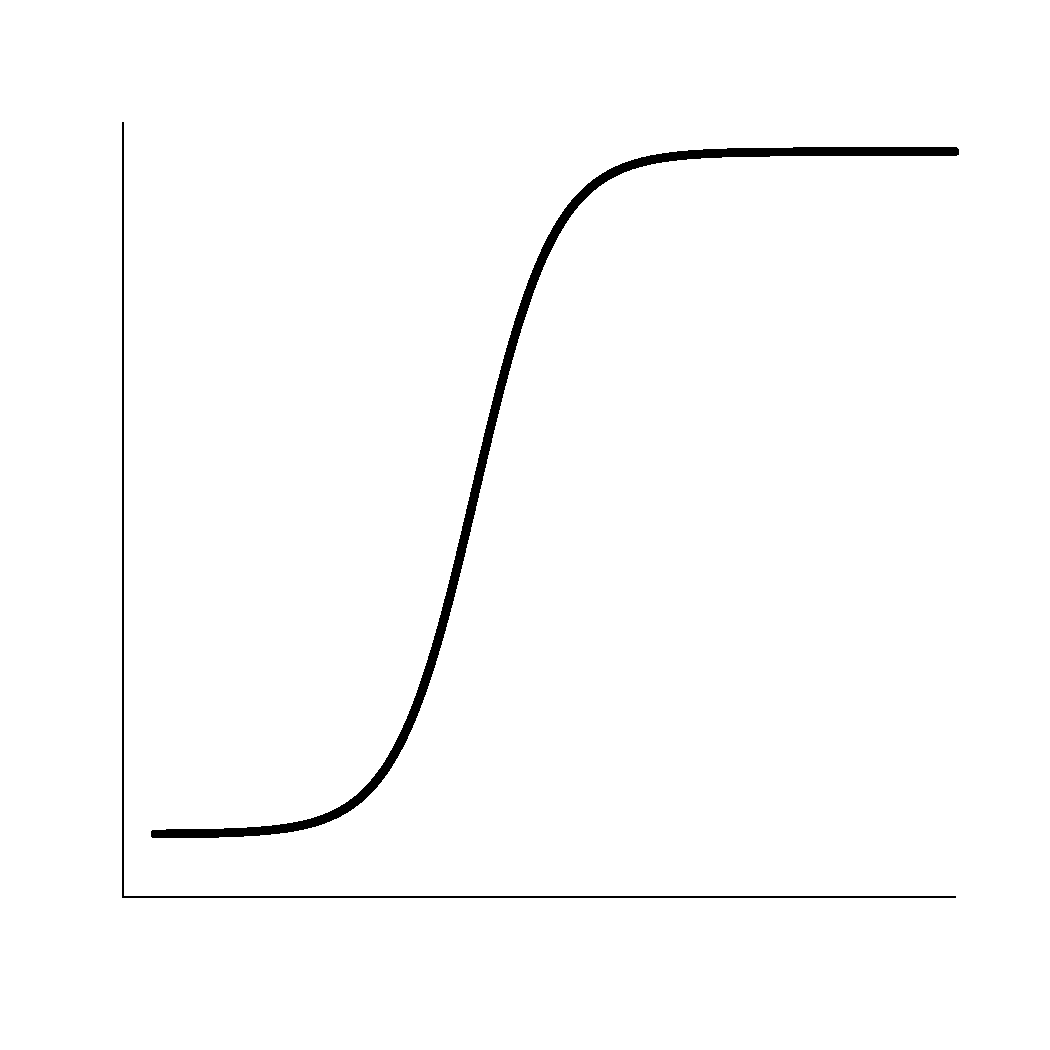
\includegraphics[width=0.45\textwidth]{logistic_a.pdf}} 
    \subfigure[]{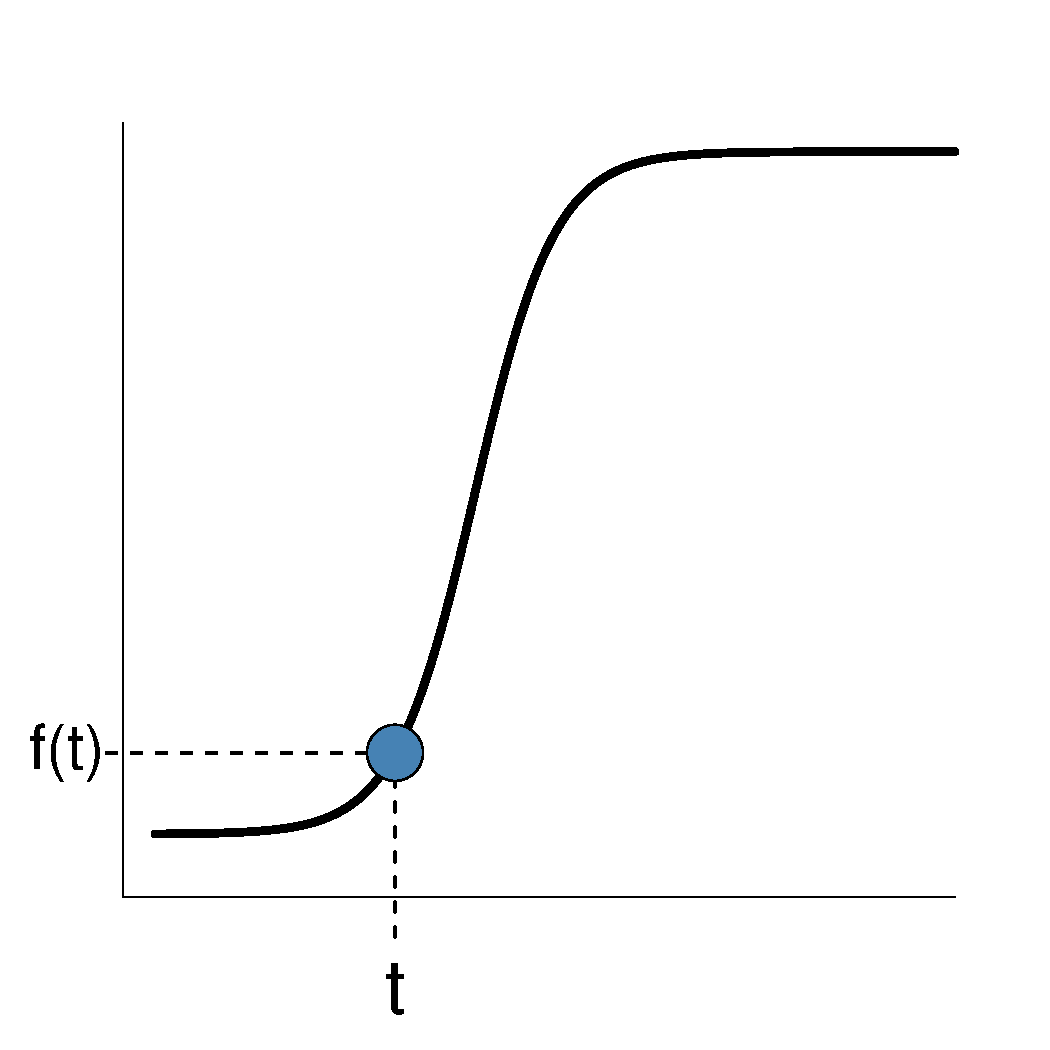
\includegraphics[width=0.45\textwidth]{logistic_b.pdf}} 
    \subfigure[]{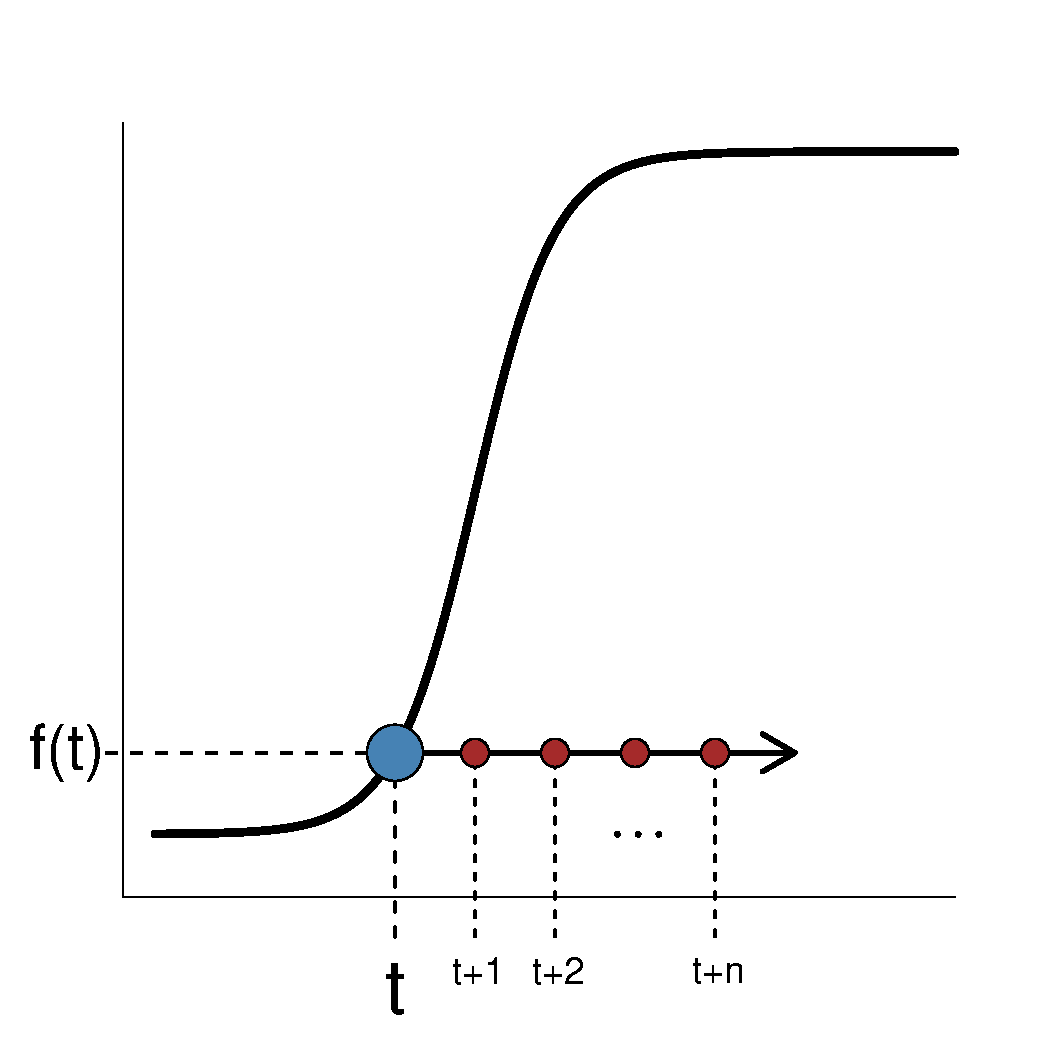
\includegraphics[width=0.45\textwidth]{logistic_c.pdf}}
    \caption{ \textbf{(a.)} Example of a nonlinear activation curve $f(t|\theta)$ \textbf{(b.)} At some time, $t$, a saccade is launched with its destination probabilistically determined by $f(t|\theta)$ \textbf{(c.)} For a look persisting over $n$ time points, $t+1, \dots, t+n$, we are recording ``observed" data, adding to the proportion of fixations at each time but without having gathered any additional observed data at $f(t+1 | \theta), \dots,f(t+n | \theta)$, thus inflating (or in the case of a monotonically increasing function like the logistic, deflating) the true probability. }
\label{fig:folly_of_fixation}
\end{figure}

To be clear, this is not to say that the length of a fixation has no relevant information regarding the strength of activation, and indeed numerous studies (source?) have demonstrated this to be the case. Rather, we argue that by more clearly specifying the particular process that we are interested in, we can perform better recovery of the underlying mechanism. (don't like this sentence).


\subsection{Delayed Observation Bias}















Because of oculomotor delay, which we define as $\rho$, a look onset observed at time $t$ is not actually determined with probability $f(t|\theta)$ but rather $f(t - \rho|\theta)$. As mentioned previously, this delay is typically acknowledged to be ``roughly" 200ms, and in a standard analysis it is usually accounted for with a horizontal shift of 200ms to the observed data. The ability to correctly specify and correct for this delay is critical, particularly in situations such as the look onset method in which the total data is much sparser and potentially much more sensitive to misspecification. 

There are two qualities of oculomotor delay that we consider here. The first is the simple observation that any difference between the true mean duration of oculomotor delay and the 200ms adjustment will result in bias. Second, we observe that in the case in which the mean duration of oculomotor delay is 200ms (and there is no bias present), the degree of randomness will have a direct effect on the observed error in the recovery of the underlying activation function. And while we don't provide any specific solutions to this problem yet, by highlighting the potential impact in simulation we demonstrate a need for further investigation.







\section{Recovery of Individual Curves}\label{sec:ind_curves}



In this section we construct a number of simulations to investigate the impact of added observation bias in the recovery of the underlying activation, as well as highlight the influence of randomness in the oculomotor delay in recovery. The simulations are constructed to emulate a typical study in the Visual World Paradigm, in which individual subjects are tasked with undergoing a series of trials, during each of which subjects make a series of fixations whose locations are probabilistically associated with lexical activation. For brevity, we consider in this section only those fixations associated with the Target object, modeled with the four parameter logistic as given in Equation~\ref{eq:logistic}; simulations according to looks to competitors is treated in the index, though the phenomenon we detail here are ultimately agnostic to any particular generating function. We will begin by detailing the process of simulating a single subject. 


\begin{figure}[H]
\centering
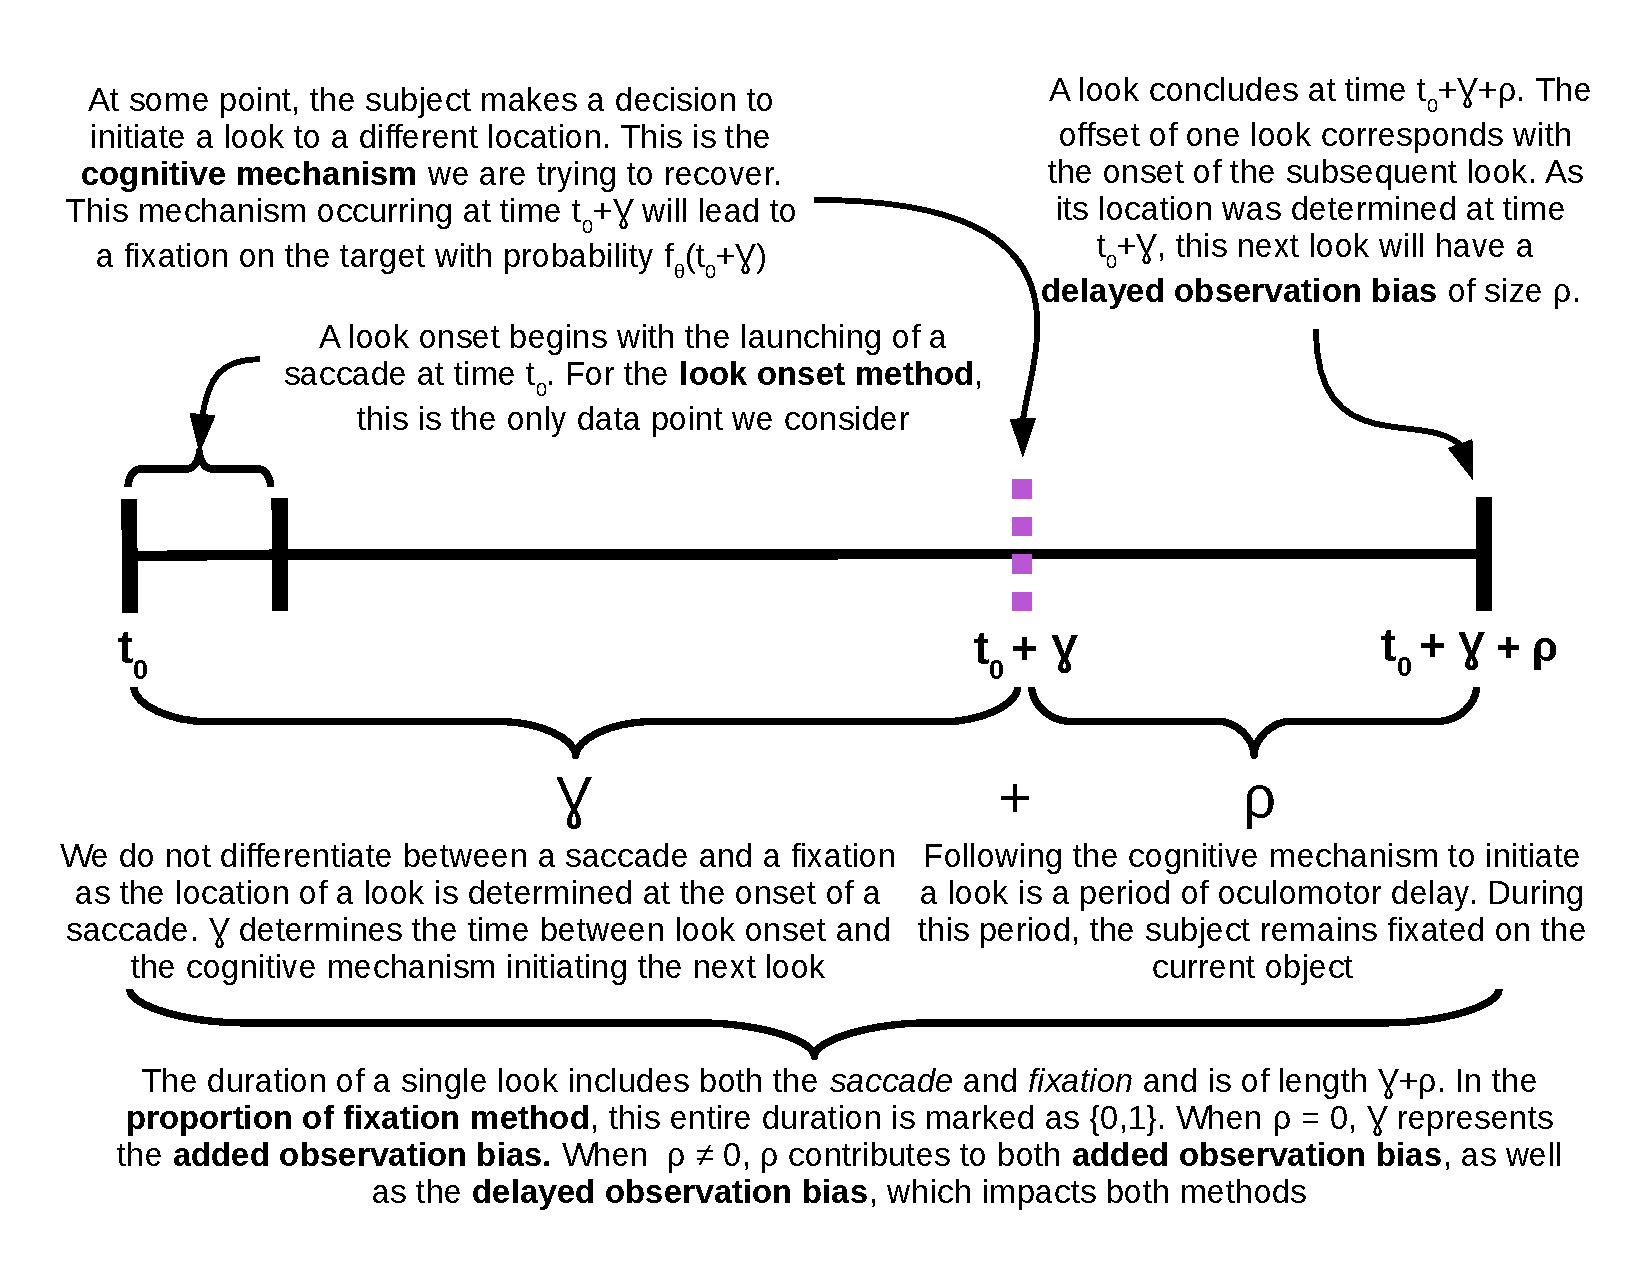
\includegraphics[width=\textwidth]{anatomy_of_look.pdf}
\caption{The Look Onset model}
\label{fig:anatomy_of_look}
\end{figure}


First, each subject $i$ randomly draws a set of parameters $\theta_i$ from an empirically determined distribution based on normal hearing participants in the VWP \cite{FarrisTrimble2014} to construct a subject specific generating curve, $f(\cdot | \theta_i)$, where $f$ here is assumed to be the logistic given in Equation~\ref{eq:logistic}.  It is according to this function that the decision to initiate a look at time $t$ will subsequently direct itself to the Target with probability $f(t|\theta_i)$. We then go about simulating trials according to the following method: At some time $t_0$, a subject initiates a look. This look persists for at least a duration of $\gamma$, drawn from a gamma distribution with mean and standard deviation independent of time and previous fixations. At time $t_0+\gamma$, the subject determines the location of its next look, with the next look being directed towards the target with probability $f(t+\gamma | \theta_i)$. The decision to initiate a look is followed by a period of oculomotor delay, $\rho$, during which time the subject remains fixated in the current location. Finally, at time $t_0 + \gamma + \rho$, the subject ends the look initiated at $t_0$ and immediately begins its next look to the location determined at time $t_0 + \gamma$. For the look onset method, the only data recorded are the times of a look onset and their location: in this case, at times $t_0$ and $t_0 + \gamma + \rho$. By contrast, the proportion of fixation method records the object of fixation at 4ms intervals for the entire period of length $\gamma + \rho$. A single trial begins at $t = 0$ and continues constructing looks as described until the total duration of looks exceeds 2000ms. Each subject undergoes 300 trials, and 1,000 subjects are included in each simulation.

Three total simulations were performed to investigate the biases identified in the previous section, each differing only in the random distribution of the oculomotor delay parameter, $\rho$. In the first simulation, we set $\rho = 0$ to remove any oculomotor delay. In this scenario, a look initiated at time $t$ by subject $i$ will be directed towards the target with probability $f(t|\theta_i)$. Doing so removes any potential bias from delayed observation and allows us to identify the effects of the added observation bias in isolation. In the remaining simulations we probe the effects of randomness in oculomotor delay, investigating what effect uncertainty may have in our recovery of the generating function. We do this assigning $\rho$ to follow either a normal or Weibull distribution, each with a mean value of 200ms. As is standard in a VWP analysis, we subtracted 200ms from each observed point prior to fitting the data. A consequence of this is that in these simulations, the bias itself is accurately accounted for by subtracting the correct mean, with the resulting error in the curve fitting process the result of the inherent variability. This does not detract from the argument being made, however, and any true bias in the mean of the oculomotor delay would asymptotically result in a horizontal shift of the observed data according to the direction and magnitude of the bias.

The simulations are performed in R, with the simulation code available on the author's Github page (github.com/collinn). Simulated data was fit to the four parameter logistic function using \xt{bdots v2.0.0}.

As all of the data could not be individually inspected prior to being included in the analysis, subjects were excluded from consideration if fitted parameters from either the look onset method or the proportion of fixation method resulted in a peak less than the slope, or if the crossover or slope were negative. In the settings in which there was no delay, normally distributed delay, or Weibull distributed delay, 981, 973, and 981 subjects were retained, respectively.





\begin{figure}[H]
\centering
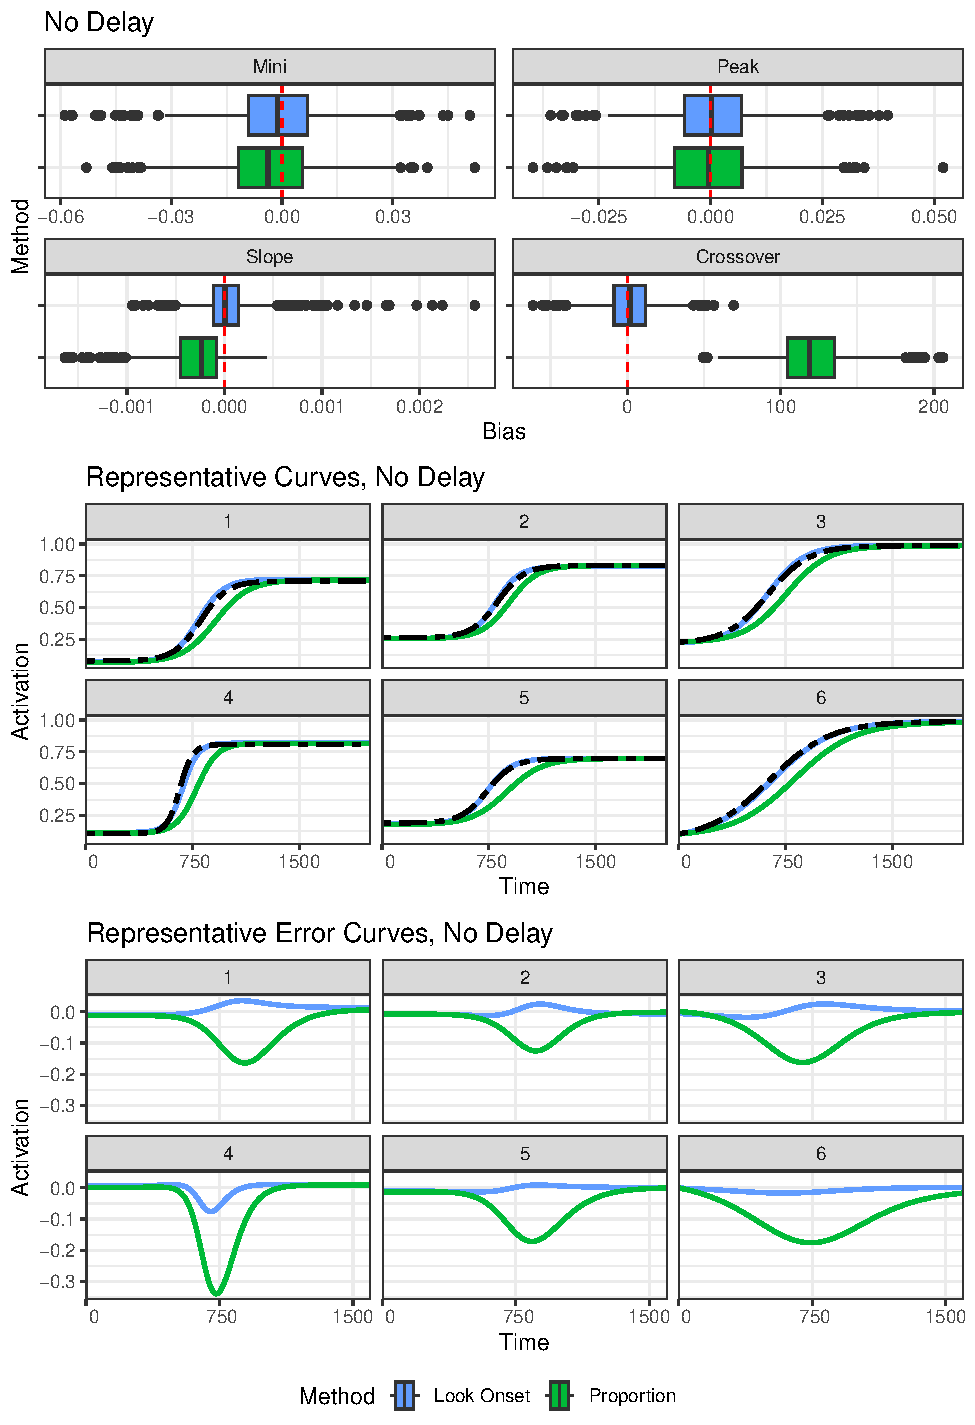
\includegraphics{rep_and_diff_no_delay.pdf}
\caption{Parameter bias with no oculomotor delay (x axis labels scrunched)}
\label{fig:par_bias_no_delay}
\end{figure}







\begin{figure}[H]
\centering
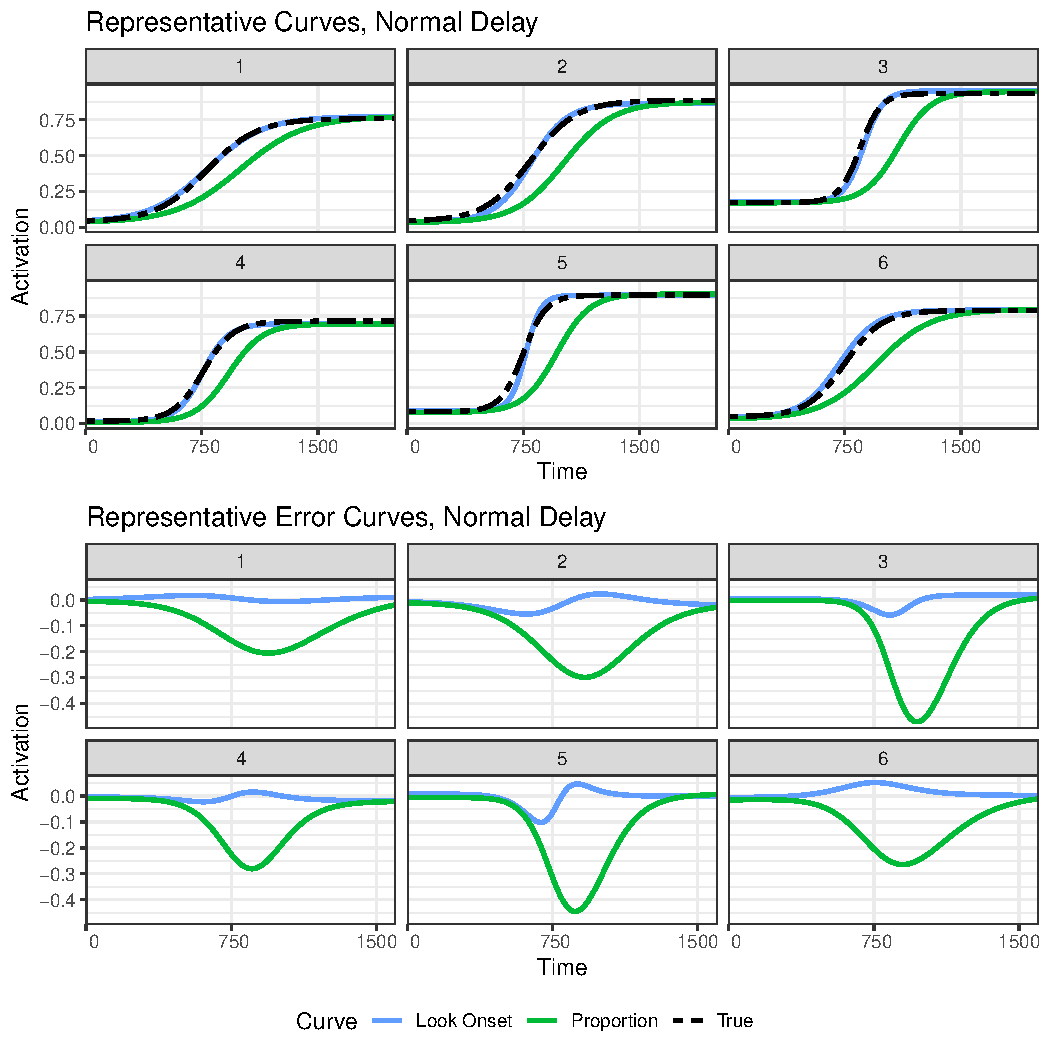
\includegraphics{rep_and_diff_normal_delay.pdf}
\caption{Representative curves with normal oculomotor delay}
\label{fig:rep_curves_normal_delay}
\end{figure}



\begin{figure}[H]
\centering
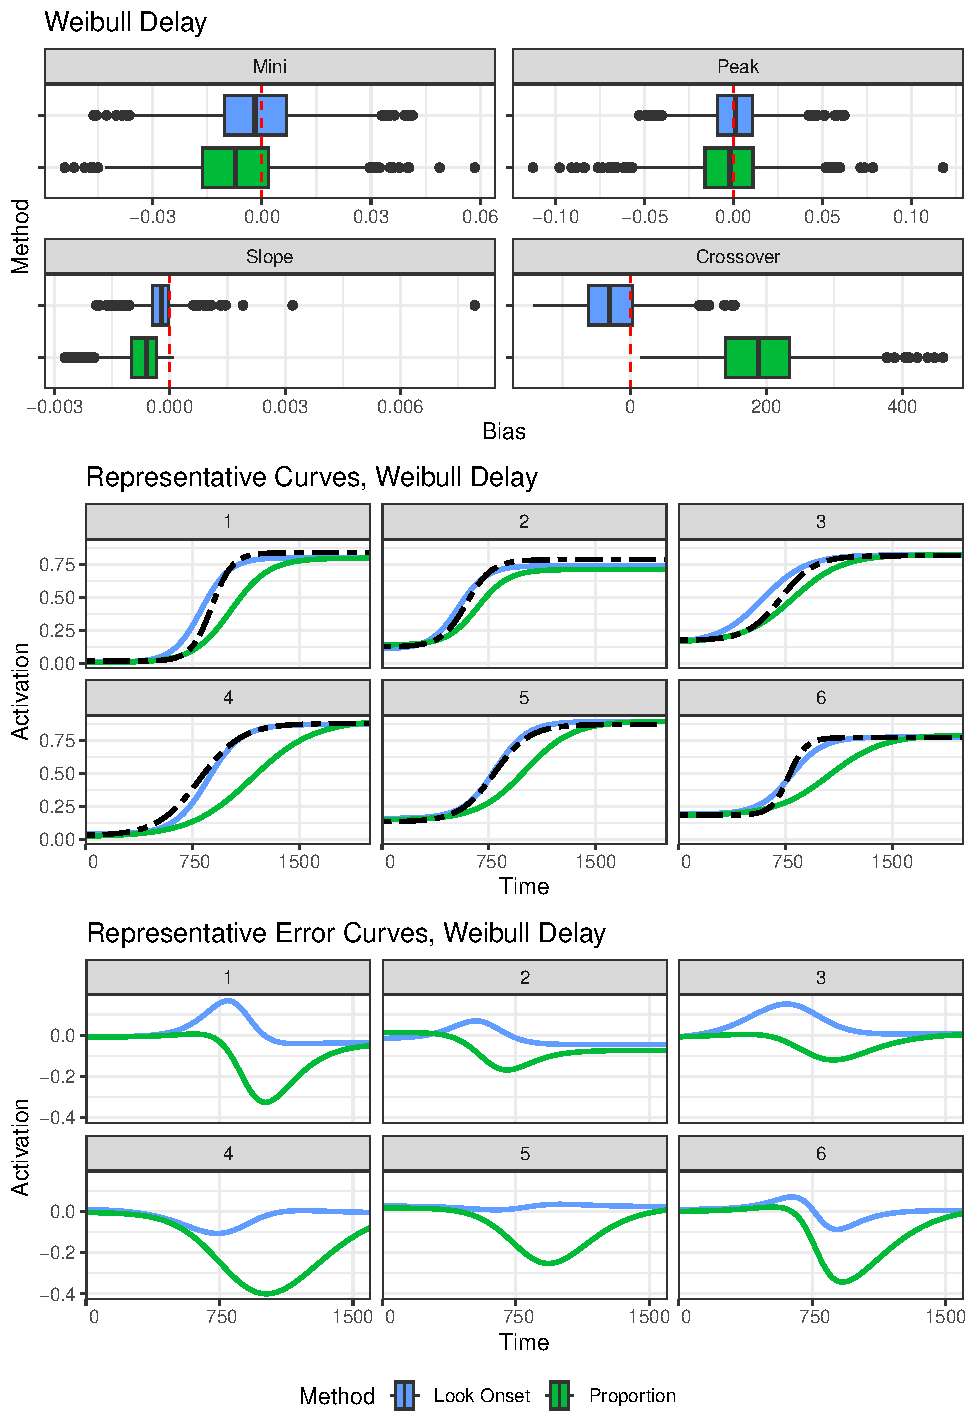
\includegraphics[width=0.9\textwidth]{rep_and_diff_weibull_delay.pdf}
\caption{Representative curves with Weibull oculomotor delay}
\label{fig:rep_curves_weibull_delay}
\end{figure}





\subsection{Results}


In addition to the visual summaries, we present in Table~\ref{tab:mise_sims} a summary of the mean integrated squared error (MISE) between the generating and recovered curves using each of the methods

We begin by noting the  magnitude of difference between the look onset method and the proportion of fixation method in the case of $\rho = 0$, or No Delay, demonstrating the amount of bias introduced in the proportion method. This alone demonstrates how critical of an issue the added observation bias is in the recovery of the underlying activation.

To assess the effects of randomness in the oculomotor delay, it seems prudent to limit the comparisons within each method. Considering first the look onset method, we see that as the degree of variability increases, so does the difficulty in correctly recovering the underlying curve. It is important to note that these magnitudes are meant to be relative rather than absolute: the particular values observed are a function of the relationship between the generating $\gamma$ distribution and that of $\rho$. Nonetheless, this does suggest a need to further investigate ways to control for the added uncertainty. To quickly comment on the apparently ``flipped" MISE for the proportion of fixation method as it relates to the normal and Weibull distributed oculomotor delay, it would seem as if the skew of the Weibull distribution acted in such a way as to actually offset some of the observed added observation bias and seems more an artifact of the simulation conditions rather than an inherent statement relating OM bias to the proportion of fixation method in general.

% latex table generated in R 4.2.2 by xtable 1.8-4 package
% Wed Feb  8 15:10:31 2023
\begin{table}[H]
\centering
\begin{tabular}{llrrr}
  \hline
Method & Delay & 1st Qu. & Median & 3rd Qu. \\ 
  \hline
Look Onset & No Delay & 0.17 & 0.32 & 0.56 \\ 
  Look Onset & Normal Delay & 0.37 & 0.71 & 1.24 \\ 
  Look Onset & Weibull Delay & 1.05 & 2.16 & 4.23 \\ 
  Proportion & No Delay & 8.21 & 11.33 & 16.01 \\ 
  Proportion & Normal Delay & 22.90 & 30.65 & 39.37 \\ 
  Proportion & Weibull Delay & 15.27 & 24.75 & 38.14 \\ 
   \hline
\end{tabular}
\caption{Summary of mean integrated squared error across simulations}
\label{tab:mise_sims}
\end{table}

The proportion of fixation method seems no longer tenable in the recovery the underlying lexical activation, given both the magnitude of differences presented in Table~\ref{tab:mise_sims} as well as the theoretical arguments made and illustrated in Figure~\ref{fig:folly_of_fixation}. And given that data collected via the look onset method can be adequately fit in the newest version of the \xt{bdots} software, there appears to be little to argue against its adoption.


\section{Recovery of Group Differences}



In Section~\ref{sec:ind_curves}, we demonstrated the utility of the look onset method in the asymptotic recovery of individual curves under our generative model. Often, however, the need to specify subject-specific differences is in pursuit of a higher goal, namely the identification of clinically relevant differences between groups. This problem is elaborated upon in \citet{mcmurray2010individual}, where it is noted, for example, that simply averaging across participants data has the ability to either create or mask group-level effects (i.e., large variability in the crossover parameter in the logistic function in Equation~\ref{eq:logistic} could manifest in the aggregate as a difference in slope). Having demonstrated the efficacy in recovering the subject-specific curves, we now consider if differences at the subject level are preserved in the aggregate through a power analysis using each of the methods discussed for identifying clinically relevant group differences. 



\begin{figure}[H]
\centering
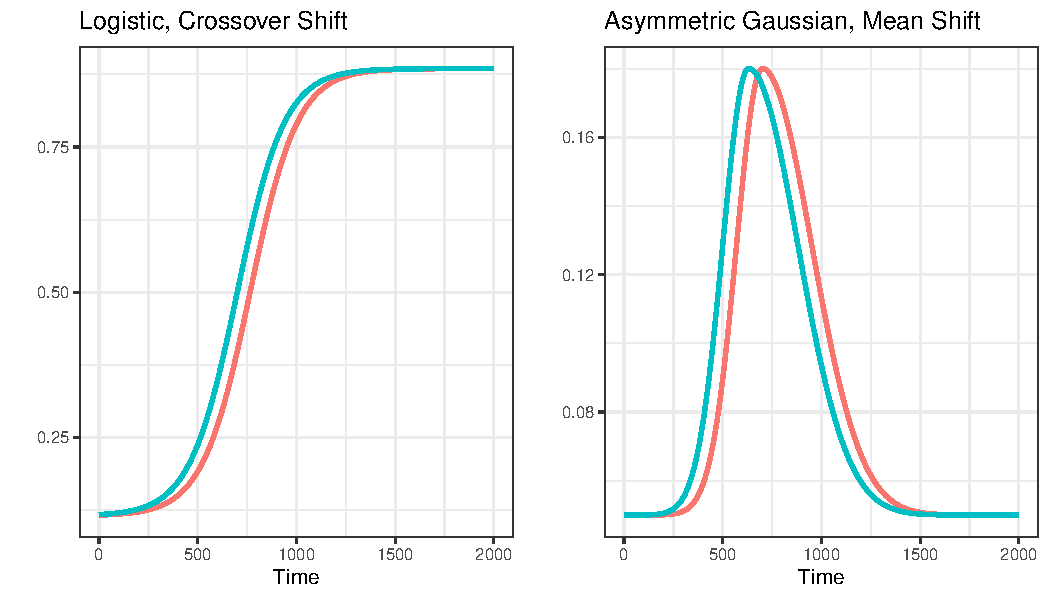
\includegraphics[width=0.9\textwidth]{group_shift.pdf}
\caption{Horizontal shift between groups}
\label{fig:group_shift}
\end{figure}

We proceed just as we did in Section~\ref{sec:ind_curves}, generating data according to the process previously described and detailed in Figure~\ref{fig:anatomy_of_look}, recovering individual curves via each the look onset and proportion of fixation methods. What differs here, however, is that each simulation is constructed to simulate drawing two groups with 25 subjects each from empirically estimated distributions that differ from one another as a horizontal shift of 65 in the location parameters (i.e., the crossover parameter in the logistic and the mean parameter in the asymmetric Gaussian). An illustration of the mean structure of each  group and its shifted counterpart is depicted in Figure~\ref{fig:group_shift}.

At first glance, the visual indication of the difference between each of the groups in Figure~\ref{fig:group_shift} can be misleading. Just as in the case of the recovery of subject-specific curves, what we are interested in here is the identification of vertical differences between groups, the magnitude of which at each time point is given in Figure~\ref{fig:difference_between_shift}. As greater differences should be easier to detect, we should anticipate a strong temporal relationship between the differences observed in Figure~\ref{fig:difference_between_shift} and the observed power.

Power for these methods is estimated in the following way: first, we simulate two groups of 25 subjects each by drawing function parameters from either the empirically determined multivariate normal distribution used in Section~\ref{sec:ind_curves} or from that same distribution with the location parameter shifted horizontally by 65. We proceed exactly the same way, both in recovering the curves under the look onset and proprotion of fixation method, and under conditions with no oculomotor delay, as well as Normally distributed and Weibull distributed delay. The fitted subject-specific curves are then used to create an estimate of the group distribution using the bootstrapping procedure in the \xt{bdots} package. Using the \xt{p\_adjust = "oleson"} adjustment for the nominal alpha, temporal regions identified as statistically significant are recorded. We repeat this process 1000 times, taking at each 4ms time point the proportion of instances in which statistically significant differences were identified.



\begin{figure}[H]
    \centering
    \subfigure[]{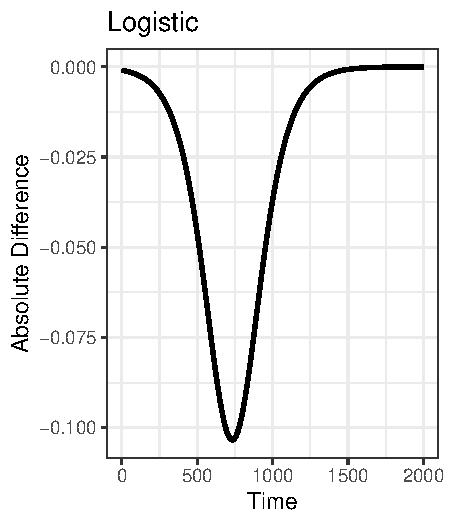
\includegraphics[]{logistic_difference.pdf}} 
    \subfigure[]{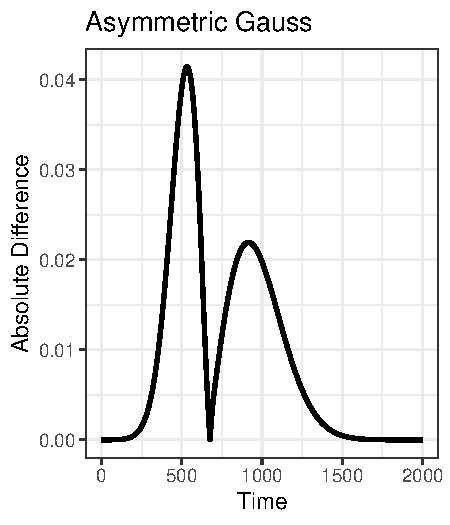
\includegraphics[]{dg_difference.pdf}} 
    \caption{Plot of error curves between shifted groups}
\label{fig:difference_between_shift}
\end{figure}

\subsection{Results}

\begin{figure}[H]
\centering
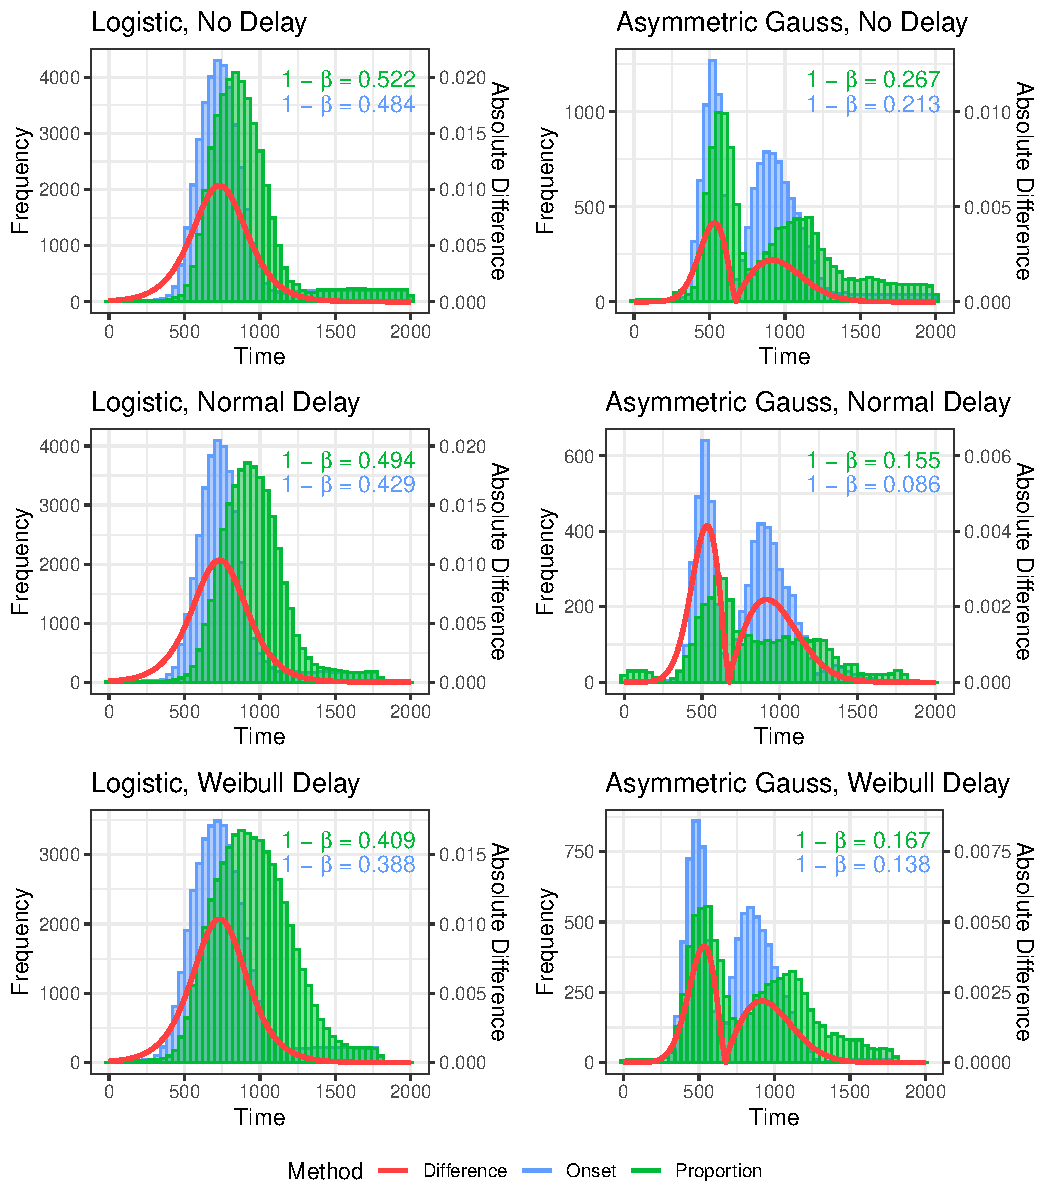
\includegraphics{diff_hist_all.pdf}
\caption{Histograms of observed power and overlaid error function}
\label{fig:diff_hist_all}
\end{figure}


Results of the simulations are presented visually in Figure~\ref{fig:diff_hist_all}. Within each tile is a histogram indicating the proportion of trials in which a statistically significant difference was identified\footnote{Binwidth for each histogram is 40, which is why some proportions are greater than 1000}. Laid over each histogram are plots of the magnitude of true differences given in Figure~\ref{fig:difference_between_shift}, helping to coordinate observed power in time. In the top right of each histogram is an estimate of total power, indicating the proportion of simulations in which \textit{any} difference was identified. Finally, the correlation between the error curve and power density for each of the setting simulations is provided in Table~\ref{tab:correlation_power}.


\begin{table}[H]
\centering
\begin{tabular}{llcc}
  \hline
Curve & Delay & Look Onset & Proportion of Fixations \\ 
  \hline
Logistic & No Delay & 0.9527 & 0.7789 \\ 
  Logistic & Normal Delay & 0.9503 & 0.5390 \\ 
  Logistic & Weibull Delay & 0.9861 & 0.6404 \\ 
  Asymmetric Gauss & No Delay & 0.9520 & 0.6554 \\ 
  Asymmetric Gauss & Normal Delay & 0.9359 & 0.6448 \\ 
  Asymmetric Gauss & Weibull Delay & 0.9413 & 0.8681 \\ 
   \hline
\end{tabular}
\caption{Correlation of power density with difference function between methods}
\label{tab:correlation_power}
\end{table}

There are several conclusions that can be readily drawn from the results presented. First, Figure~\ref{fig:diff_hist_all} demonstrates that in each case, the observed overall power was greater for the look onset method. In conjunction with this is the observation that the magnitude of temporal power in the look onset method closely matches the magnitude of absolute difference, which is corroborated by the correlations presented in Table~\ref{tab:correlation_power}. A corollary of this observation is that clinically relevance differences that are detected by the proportion of fixation method may be temporally misaligned. 




\section{Application to Real Data}

While improved performance in the theoretical domain is a necessary condition for the adoption of the look onset method, it is not sufficient, and towards that end we turn our attention now to an application with real data. We revisit here a study conducted by \cite{mcmurray2010individual}, which collected VWP data on 93 children differing in language and cognitive abilities. This included children who were typically developed (N, $n = 40$), those with specific language impairment (SLI, $n = 20$) and non-specific language impairment (NLI, $n = 17$), and those with specific cognitive impairment (SCI, $n = 16$). Though the primary goals of this study involved both the investigation of individual differences and the mapping of particular physiological characteristics to TRACE parameters, we limit our consideration here to a standard analysis in \xt{bdots} whereby we seek to identify temporal-specific differences in the trajectory of fixations with looks to the Target, modeled with the four parameter logistic function. We do this by structuring the original data according to both the proportion of fixations and look onset methods, fitting subject-specific curves to the data, and then identifying statistically significant differences via permutation testing in \xt{bdots}. As there are four total groups, we consider each of the pairwise differences, resulting in six total differences for investigation.

\subsection{Data Preparation}

There are a number of decisions that must be made when transforming raw eye tracking data to a format suitable for the look onset method. Briefly, we detail here the decisions made in processing data for both the proportion of fixations and for look onset. First, in all cases we removed trial data in any trials for which the subject made no fixations or selected the incorrect object in response to the auditory signal. We recorded no fixations or saccade movements (for look onset) that occurred past 2300ms, and we truncated data in each trial to end once the participant had selected the correct response.

For look onset data specifically, there are a number of additional decisions to be made, particularly regarding the beginning and end of an individual trial. At the beginning of a trial when $t = 0$, for example, the eyes are already fixated on some location (typically the center), yet these are accounted for in the proportion of fixation. Regarding look onset, we must then decide whether we choose to take the first saccade launched after the beginning of the trial, resulting in a paucity of data near the beginning, or to choose to include the first saccade launched prior to the beginning of the trial which would be unrelated to the auditory stimulus (as it had not yet been received), but would offer more consistency with the data provided via the proportion of fixations. Similarly, one notes that at the end of a trial, a fixation will persist until the response has been collected (resulting in ``observed" data), whereas the final saccade launched prior to response will often be a few hundred milliseconds sooner, resulting in a similar paucity of data at the end of the trial. Ultimately, we elected to only include saccades launched after the onset of auditory stimulus and made no further accommodation for the end of the trial, and although our results were not sensitive to either of these decisions, we believe they are worth consideration in future work.


\subsection{Results}

\begin{figure}[H]
    \centering
    \subfigure[]{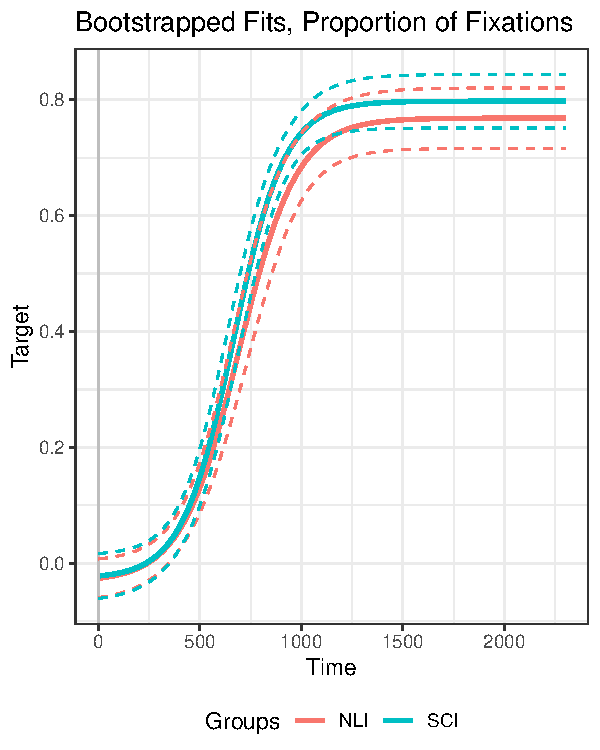
\includegraphics[width=0.48\textwidth]{irl_data_prop_1.pdf}}
    \subfigure[]{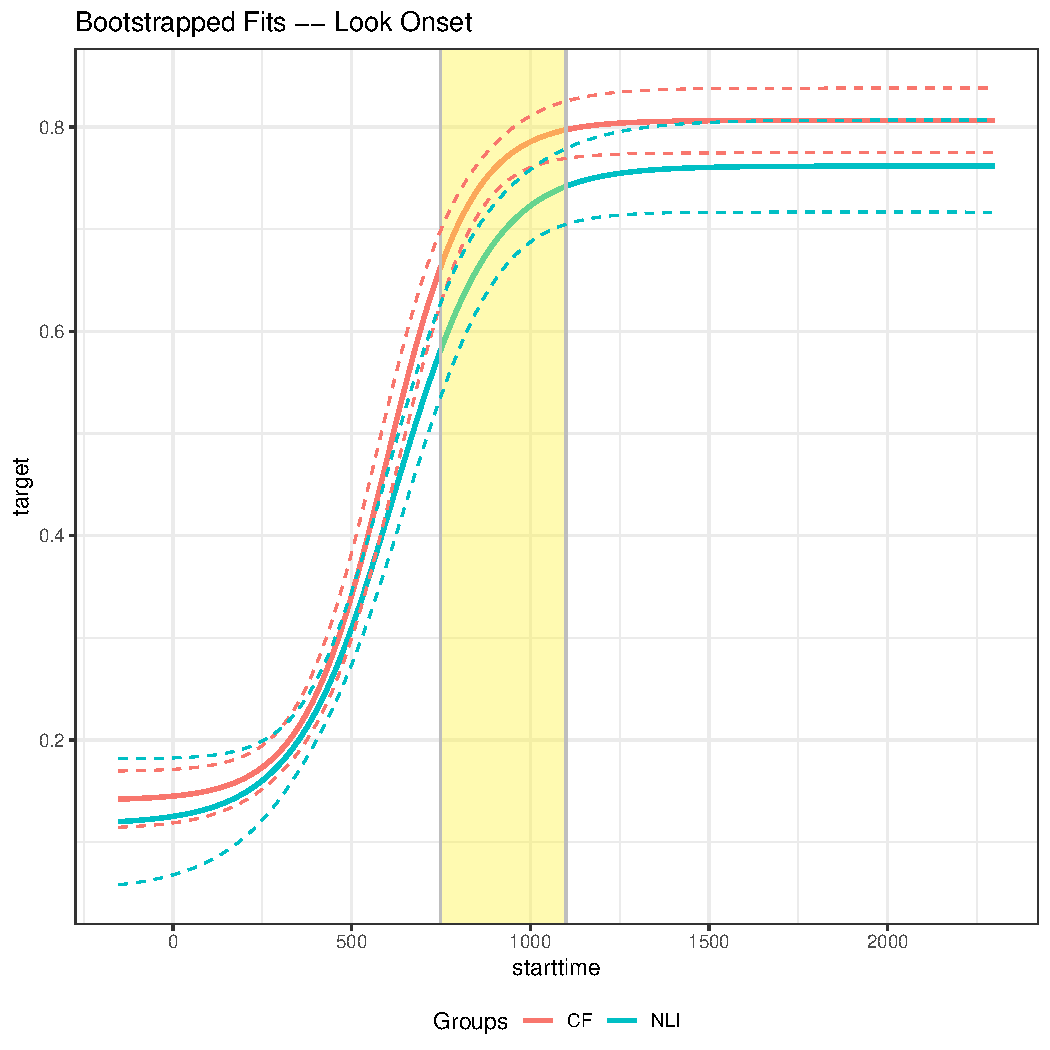
\includegraphics[width=0.48\textwidth]{irl_data_onset_1.pdf}}
    \caption{Estimated mean curves with confidence intervals of NLI and SCI, with significant region identified using the look onset method}
\label{fig:irldata1}
\end{figure}

Temporal differences between groups were made using permutation testing in \xt{bdots}. Of the six comparisons made, only two were found to have significant differences between group curves, those being the comparisons made between specific cognitive impairment (SCI) and non-specific language impairment (NLI), as well as between NLI and typically developed adolescents (N). Further, these differences were only identified with the look onset method, with the proportion of fixation method in both cases offering null results. Plots of the mean curves and bootstrapped confidence intervals, along with highlighted regions of identified differences, are provided in Figure~\ref{fig:irldata1} and Figure~\ref{fig:irldata2}.



\begin{figure}[H]
    \centering
    \subfigure[]{
\includegraphics[width=0.48\textwidth]{irl_data_prop_2.pdf}}
    \subfigure[]{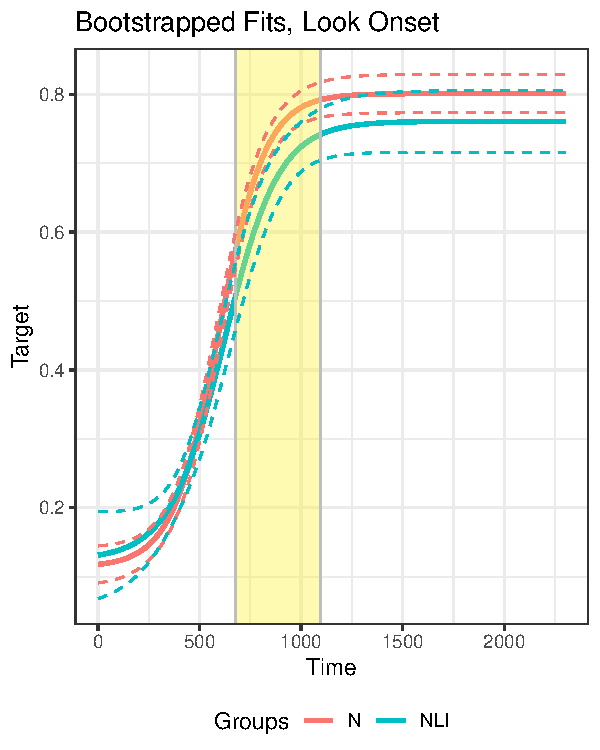
\includegraphics[width=0.48\textwidth]{irl_data_onset_2.pdf}}
    \caption{Estimated mean curves with confidence intervals of NLI and N, with significant region identified using the look onset method}
\label{fig:irldata2}
\end{figure}



\section{Discussion}



Through our investigation, we have presented a physiologically grounded model relating eye tracking data to underlying lexical access by placing emphasis singularly on the first instance of a look. Under the assumptions of this model, we further demonstrated a significant source of bias present under the standard ``proportion of fixations" method typical of VWP data. We have proposed an alternative in response, the look onset method, which limits relevant data to the initial launching of a saccade. Under our generative model, we not only demonstrated superior recovery of individual subject-specific curves but also in the unbiased identification of temporal-specific differences between groups. The utility of this additional power was made evident in our re-examination of an existing study, in which the look onset method identified several statistically significant differences between groups, whereas the proportion of fixation method did not. And finally, the look onset method can be implemented immediately, utilizing the same analytic approach provided by the \xt{bdots} package in R.

The look onset method has the further benefit of giving rise to a much sparser dataset, providing a more computationally tractable basis for algorithms with complexity which scale in the number of observations. This may be of considerable advantage in fitting mixed models to the data, potentially providing the ability to control for trial-specific variability, an option that has hitherto been infeasible. 

Of likely concern to many readers will be the fact that, as the look onset method retains only the initial onset of a fixation, a great deal of information is lost concerning the \textit{duration} of the fixation. It is well established \citep{Salthouse1980} that the length of a fixation is itself meaningful, with longer fixations generally associated with stronger activation. The length of fixation may also be important when attempting to differentiate fixations associated with searching patterns (i.e., what images exist on screen?) against those associated with consideration (is this the image I've just heard?). It would be incorrect to suggest that the look onset method considers the length of fixation \textit{irrelevant}; rather, it makes no statement about it at all. In other words, by clearly delineating two separate processes, one initiating an eye movement, the other determining the duration, we free ourselves to construct far more nuanced models. For example, the length of a fixation may suggesting a weighting to the proceeding look onset, with a longer duration being indicative of intentional consideration and shorter ones being suggestive of searching behavior. These questions suggest a number of experimental designs to differentiate eye tracking behavior, particularly with regards to scanning/search behavior and experimental conditions, similar to what is demonstrated in \citep{Apfelbaum2021}.


It is also critical to specify a present shortcoming in how the duration of fixations are treated. Implicit in the proportion of fixations method is a crucially overlooked assumption of a linear relationship between the fixation length and the activation. That is, insofar as the construction of the fixation curve is considered, a fixation persisting at 20ms after look onset (and well within the refraction period in which no new information regarding the cognitive mechanism or voluntary fixation could be obtained, see Figure~\ref{fig:whats_in_a_look}) is considered identical to a fixation persisting at 500ms after onset: both are undifferentiated in being recorded as either a $0$ or $1$. In other words, the specific duration of a particular fixation does not directly change how the data is recorded. This is in contrast to the possibility offered by the look onset method, whereby the duration of the fixation could weight the look onset by importance.

A second consideration necessary for using the length of a fixation is the composition of the fixation itself, given in Figure~\ref{fig:whats_in_a_look}. Suppose, for example, that the refractory period following each fixation was exactly 100ms and that the oculomotor delay before initiating the subsequent fixation is exactly 200ms. From this, we could conclude that 300ms of any fixation are ``built in" and have no necessary information regarding the strength of activation motivating the fixation. Without considering this information, we may determine a fixation of 500ms to be 25\% greater than a fixation of 400ms. However, once we account for the ``built in" portion of a fixation, we see that the first is associated with an intentional fixation period of 200ms, whereas the second has an intentional period of only 100ms. In this light, the first fixation might be considered 100\% greater than the latter. And while we offer no more than speculation here, this phenomenon should be taken into consideration in future research.

In conclusion, we have presented a statistically defensible generative model for eye movements in the context of the Visual World Paradigm, accompanied by a novel method for aggregating and analyzing collected data. While the methods proposed are not a drastic alteration to the motivating assumptions of \citet{allopenna1998tracking}, we believe them to be a critical step forward towards a statistically sound treatment of eye tracking data in the realm of lexical activation.




\section*{Appendices}


\section{Misc OM Discussion}


Outside of a demonstration of its existence and potential consequence, little more has been said about addressing the delayed observation bias. Further, the consequences of the delayed observation (under the assumption that the mean value is correctly accounted for) seem almost trivial in comparison to the differences between it and the added observation bias. That being said, we believe there are still critical reasons for considering its significance.

As mentioned earlier, the particular values observed in these simulations are both a function of the relationship between the distribution generating $\gamma$ and that of $\rho$. However, they are also a function of the generating function itself. In particular, we draw attention to the degree of total variation $f$ over the interval $[a,b]$, defined as 

\begin{equation}
V(f) = \underset{\mathcal{P}}{\sup} \sum_{i=0}^{n_p-1} \left|f(t_{i+1}) - f(t_i) \right|,
\end{equation}

where $\mathcal{P} = \{P = \{t_0, \dots, t_{n_p}\} \}$ is the set of all possible partitions of $[a,b]$. Despite appearances, this is a relatively straightforward metric in the case of monotone functions such as the logistic, where the total variation is simply $|f(b) - f(a)|$. To illustrate the relevance of this, consider a hypothetical situation in which the underlying activation we are wishing to recover is a constant function, $f(t) = c$, where the probability of fixating on a target is independent of time. In such a situation, a delayed observation would be of no issue; despite changes in time $t$, the probability $c$ remains unchanged. In contrast, consider a second hypothetical situation in which activation is defined exponentially, $f(t) = \exp(t)$. In this case, the impact of delayed observation depends drastically on time, when the delay in observation in the range of small values of $t$ have a drastically smaller impact than delayed observations when $t$ is large ($\exp(1) - \exp(0) = 1.7183$ while $\exp(11) - \exp(10) = 37848$, despite both cases having $\Delta t = 1$).

In short, these hypothetical situations detail how the magnitude of total variation can have differential effects on the delay in observation. Now consider again the logistic function in Figure~\ref{fig:logistic_definition} and imagine its domain partitioned into three equally sized portions. Both the first and third, near the asymptotes, have relatively low total variation, resulting in a relatively benign effect from oculomotor delay. In contrast, the middle third contains nearly all of the variation of the function, indicating the delayed observation here will have a disproportionate impact on the successful recovery of the function. Given the clinical relevance of the both the slope and crossover parameters, as well as acknowledging the impact that these have on the overall shape of the function, we demonstrate a need in a accounting for this delay precisely where it will impact function recovery the most. This, of course, is not unique to the logistic, with the effects of the delayed observation bias compounded in the asymmetric Gaussian functions (appendix) which has a more complicated variation structure and, accordingly, more difficulty in recovering the generating curves.


\section{Recovery of Individual Curves -- Asymmetric Gaussian}

Presented here are the results of the simulations for the recovery of subject-specific curves generated with the asymmetric Gaussian function, the parametric function typically associated with looks to competitors in the VWP. As in the section fitted with the logistic function, simulations include settings in which there is no oculomotor delay, as well as delay that is normally and Weibull distributed. Again, as all fits could not be individual examined, an automated criterion was used to determine which fits were considered  adequate. Here, this stipulated that the estimated sigma parameters be positive and that the height parameter be larger than either of the base parameters. The number of fits retained for the no delay, normal delay, and Weibull delay were  855, 786, and 816, respectively.


\subsection{Results}

As might be expected, the more complicated mean structure provided by the asymmetric Gaussian led to a generalized increase in the difficulty of recovery for both the look onset and proportion methods, relative to those generated with a logistic mean structure. However, we do still find that in the case of no delay, given in Figure~\ref{fig:dg_rep_curves_no_delay}, that the recovery of individual parameters is still unbiased and, as with the logistic, the location parameter (here, mu), is right shifted.

The results for the median integrated squared error are given in Table~\ref{tab:dg_mise_sims}. We again see results similar to those with the logistic in that the look onset method outperforms the proportion of fixation method in all cases. 

\begin{figure}[H]
\centering
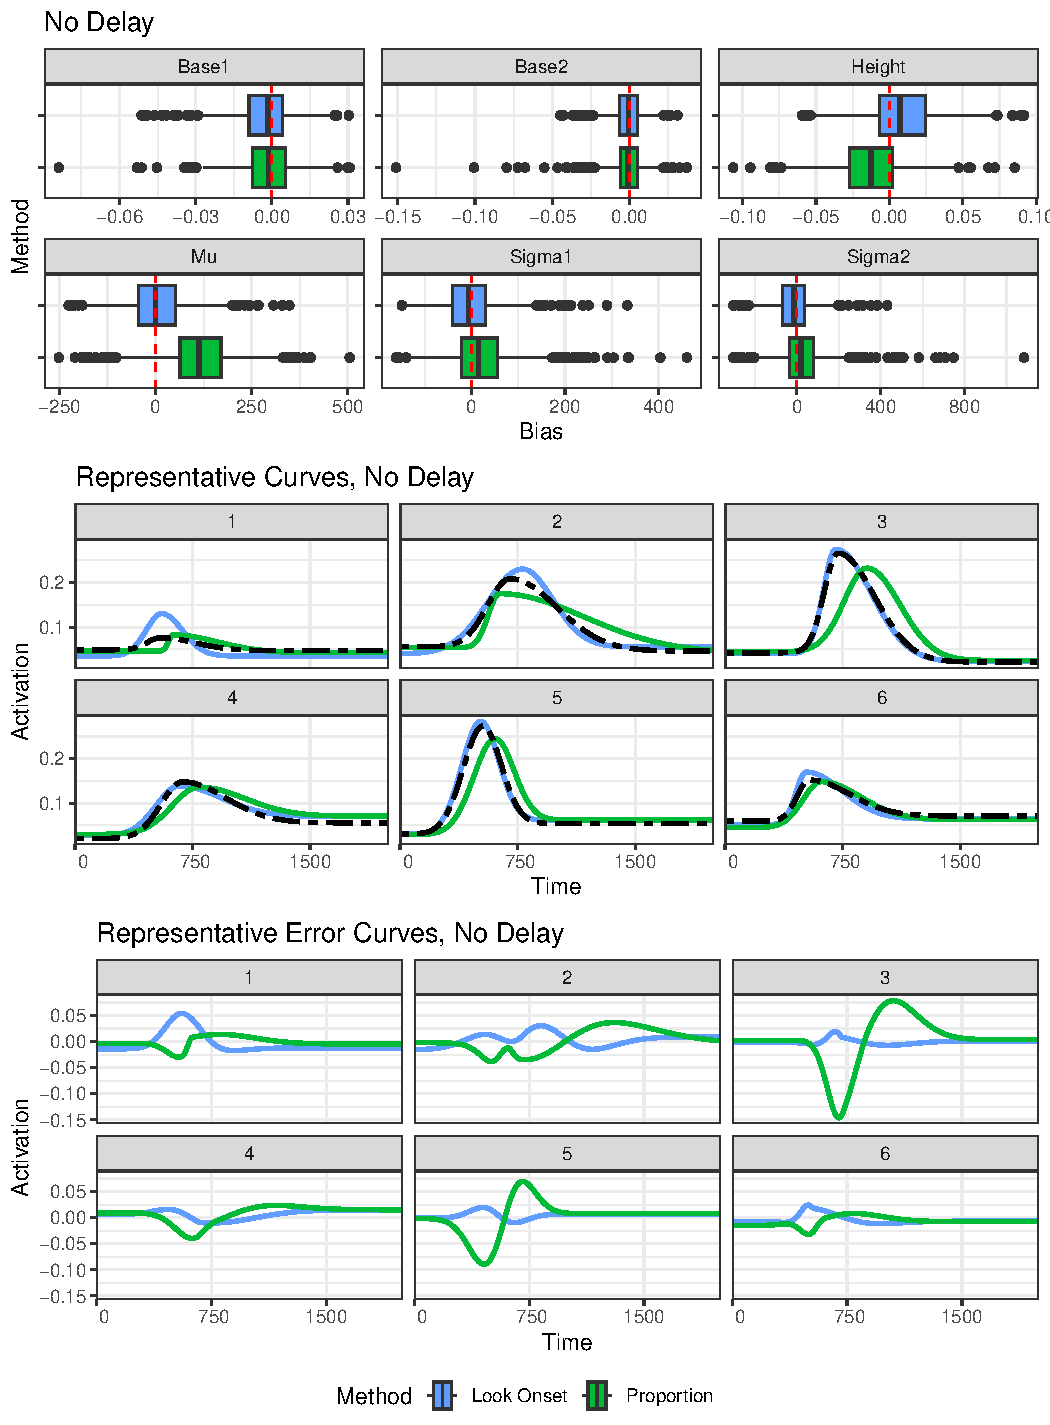
\includegraphics[width=0.9\textwidth]{dg_rep_and_diff_no_delay.pdf}
\caption{Summary of simulation results in the recovery of subject-specific curves generated by the asymmetric Gaussian with no oculomotor delay}
\label{fig:dg_rep_curves_no_delay}
\end{figure}

\begin{figure}[H]
\centering
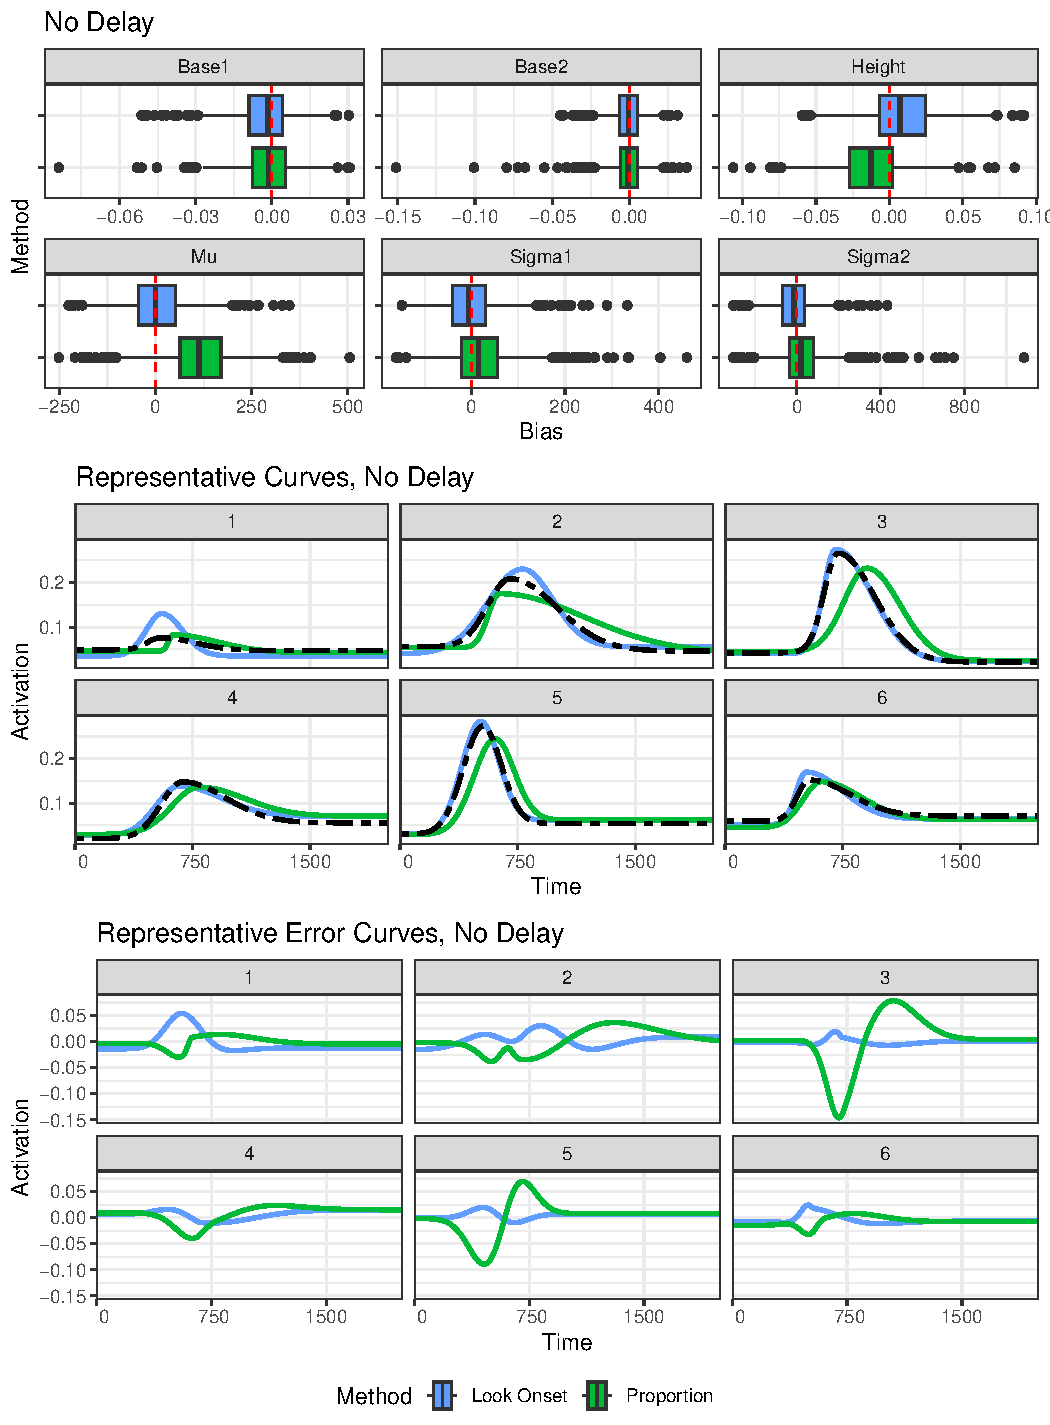
\includegraphics[width=0.9\textwidth]{dg_rep_and_diff_no_delay.pdf}
\caption{Summary of simulation results in the recovery of subject-specific curves generated by the asymmetric Gaussian with normally distributed oculomotor delay}
\label{fig:dg_rep_curves_normal_delay}
\end{figure}


\begin{figure}[H]
\centering
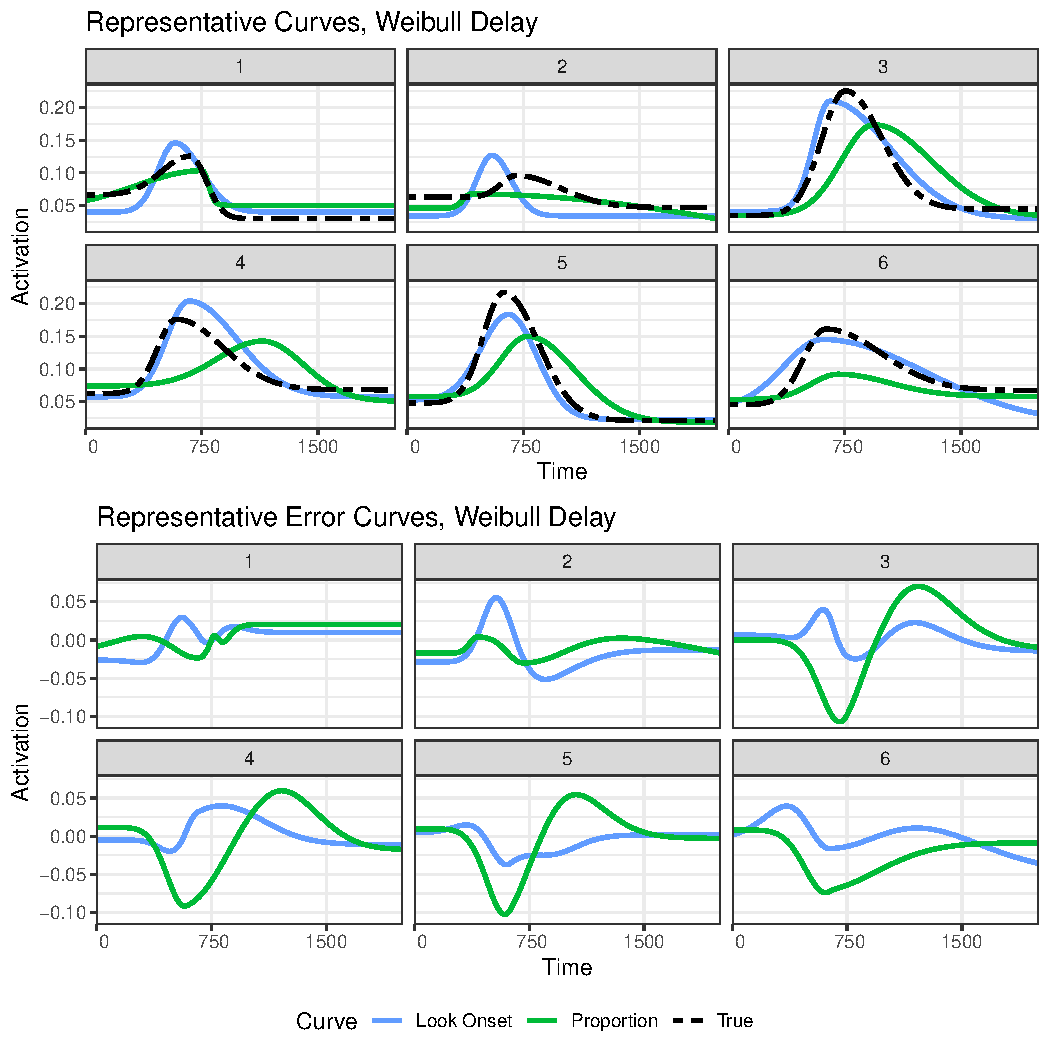
\includegraphics[width=0.9\textwidth]{dg_rep_and_diff_weibull_delay.pdf}
\caption{Summary of simulation results in the recovery of subject-specific curves generated by the asymmetric Gaussian with Weibull distributed oculomotor delay}
\label{fig:dg_rep_curves_weibull_delay}
\end{figure}




\begin{table}[H]
\centering
\begin{tabular}{llrrr}
  \hline
Curve & Delay & 1st Qu. & Median & 3rd Qu. \\ 
  \hline
Look Onset & No Delay & 0.22 & 0.36 & 0.63 \\ 
  Look Onset & Normal Delay & 0.38 & 0.70 & 1.15 \\ 
  Look Onset & Weibull Delay & 0.52 & 0.84 & 1.39 \\ 
  Proportion & No Delay & 0.75 & 1.29 & 2.08 \\ 
  Proportion & Normal Delay & 1.38 & 2.44 & 3.96 \\ 
  Proportion & Weibull Delay & 1.00 & 1.98 & 3.43 \\ 
   \hline
\end{tabular}
\caption{Median integrated squared error for recovery of individual curves generated with asymmetric Gaussian}
\label{tab:dg_mise_sims}
\end{table}

\subsection{$R^2$ for Recovery of Individual Curves}

Here, we provide an alternative summary of the recovery of subject specific curves fit with both the logistic and asymmetric Gauss. 


\subsubsection{Logistic}

\begin{table}[H]
\centering
\begin{tabular}{llrrr}
  \hline
Curve & Delay & 1st Qu. & Median & 3rd Qu. \\ 
  \hline
Look Onset & No Delay & 1.00 & 1.00 & 1.00 \\ 
  Look Onset & Normal Delay & 0.99 & 1.00 & 1.00 \\ 
  Look Onset & Weibull Delay & 0.98 & 0.99 & 0.99 \\ 
  Proportion & No Delay & 0.92 & 0.94 & 0.95 \\ 
  Proportion & Normal Delay & 0.80 & 0.83 & 0.86 \\ 
  Proportion & Weibull Delay & 0.80 & 0.86 & 0.91 \\ 
   \hline
\end{tabular}
\caption{$R^2$ for Logistic}
\label{tab:r2_logistic_sims}
\end{table}

\subsubsection{Asymmetric Gaussian}

\begin{table}[H]
\centering
\begin{tabular}{llrrr}
  \hline
Curve & Delay & 1st Qu. & Median & 3rd Qu. \\ 
  \hline
Look Onset & No Delay & 0.80 & 0.91 & 0.95 \\ 
  Look Onset & Normal Delay & 0.63 & 0.82 & 0.91 \\ 
  Look Onset & Weibull Delay & 0.57 & 0.77 & 0.87 \\ 
  Proportion & No Delay & 0.48 & 0.65 & 0.75 \\ 
  Proportion & Normal Delay & 0.10 & 0.33 & 0.52 \\ 
  Proportion & Weibull Delay & 0.20 & 0.46 & 0.64 \\ 
   \hline
\end{tabular}
\caption{$R^2$ for Asymmetric Gaussian}
\label{tab:r2_dg_sims}
\end{table}








\newpage

\Chapter{With great power comes greater responsibility}
\section{Introduction}

A standard problem in psycholinguistics, and the cognitive sciences in general, is that of statistically analyzing a process unfolding in time. Particularly in the case of comparing a process between experimental groups in time, techniques appropriate for demonstrating showing that differences \textit{exist} offer little towards the goal of identifying \textit{when} they exist when the time windows are not specified in advance, with the area under a curve (AUC) representing an example of this. One may consider instead testing two time series at each point in time, using a method such a cluster based permutation testing \cite{Maris2007} in which test-statistics are computed at each time, with adjacent significant tests being combined into single clusters. This is in an effort to address the problem of multiple comparisons and, by extension, control for the family wise error rate (FWER): by reducing adjacent test statistics into a single cluster, researchers work to control the FWER by simply reducing the number of tests. More recently has been the bootstrapped differences of time series (BDOTS) \cite{oleson2017detecting}, using bootstrapped fits of subject-level curves in conjunction with a modified Bonferroni correction to the significance level to control the family wise error rate in the presence of highly correlated test statistics. A version of this was introduced in the R package \xt{bdots} in 2018 \cite{seedorff2018bdots}.

A closer look at the specific conditions under which the original iteration of \xt{bdots} was presented raises concerns, however, involving quite restrictive assumptions that are unlikely to be met in many, if not most, situations. This includes data typically collected in the Visual World Paradigm (VWP), context in which the underlying methodology was first proposed. Specifically, it assumed a homogeneous mean structure within each of the groups being compared, with no between-subject variability to be accounted for. Empirical data collected in a variety of (VWP) contexts can be used to show that such an assumption is unlikely to be true, with the resulting type I error rate being unacceptably high.

What we present instead is two alternatives, accommodating flexibility in two of the assumptions made in the original bdots. First, we propose a modified bootstrapping procedure that adequately accounts for observed between subject variability while retaining the FWER adjustment method presented for autocorrelated errors. In addition, we offer a permutation test between the groups, borrowing from the insight of the original bdots in that it also captures within-subject variability as demonstrated in the standard errors in the model fits. We begin by describing the two proposed alternatives to the original bdots bootstrap. We then outline the details of the simulations in demonstrating the type I error rate across a number of experimental conditions, and finally we conclude with a demonstration of power in the competing methods.


\section{Detail on the original}

Most generally the original bdots algorithm, which we will call the \textit{homogeneous bootstrap}, proposed that we have empirically observed data in time resulting from a parametric function $f$ with an associated error: 

\begin{equation}\label{eq:mean_structure}
y_{t} = f(t|\theta) + \epsilon_{it}
\end{equation}
where 
\begin{equation}
\epsilon_{it} = \phi \epsilon_{i, t-1} + w_{it}, \quad w_{it} \sim N(0, \sigma).
\end{equation}
Under this paradigm, the errors could be iid normal (with $\phi = 0$) or have an AR(1) structure, with $0 < \phi < 1$. It further assumes homogeneity of the mean structure, meaning that two subjects from the same group would have parameters $\theta_{it} = \theta_{jt}$ for all $i, j$. In other words, it was assumed that there was no variability in the mean structure between subjects in the same group. \cn{This is also evidenced in the original bdots algorithm: }

%\begin{singlespace}
\begin{enumerate}
\vspace{-3mm}
\item[1.] For each subject, fit the nonlinear function, specifying AR(1) autocorrelation structure for model errors. Assuming large sample normality, the sampling distribution of each estimator can be approximated by a normal distribution with mean corresponding to the point estimate and standard deviation corresponding to the standard error

\item[2.] Using the approximate sampling distributions in (1.), randomly draw one bootstrap estimate for each of the model parameters on every subject

\item[3.] Once a bootstrap estimate has been collected for each parameter and for every subject, for each parameter, find the mean of the bootstrap estimates across individuals

\item[4.] Use the mean estimates to determine the predicted population level curve, which provides the average population response at each time point

\item[5.] Perform steps (2)-(4) 1000 times to obtain estimates of the population curves. Use these to create estimates of the mean response and standard deviation at each of the time points. 
\end{enumerate}
%\end{singlespace}

Population means and standard deviations at each time point for each of the groups were used to construct a series of (correlated) test statistics, where the family wise error rate was controlled by using the modified Bonferonni correction introduced in \cite{oleson2017detecting} to test for significance.


\section{Proposed Methods}

As is more typically the case, subjects within a group demonstrate considerable variability in their mean parameter estimates. In such a case, there is no presumption that $\theta_i = \theta_j$, and accounting for between-subject variability within a group will be critical for obtaining a reasonable distribution of the population curves.

\subsection{Modified Bootstrap}

\cn{A more likely case involving subjects in the VWP (or subjects within any group exhibiting between and within subject variability) is as such: }

The distribution of parameters for subjects $i = 1, \dots, n_g$ in group $g = 1, \dots, G$ follows the distribution

\begin{equation}\label{eq:theta_i_dist}
\theta_i \sim N(\mu_{g}, V_{g}).
\end{equation}

The uncertainty present in our estimation of $\theta_i$ can be accounted for by treating the standard errors derived when fitting the observed subject data to Equation~\ref{eq:mean_structure} as estimates of their standard deviations. This gives us a distribution for the subject's estimated parameter, 

\begin{equation}
\hat{\theta}_i \sim N(\theta_i, s_i^2).
\end{equation}

When obtaining reasonable estimates of the population curve, it is necessary to estimate both the observed within-subject variability found in each of the $\{s_i^2\}$ terms, \textit{as well as} the between-subject variability present in $V_{g}$. For example, let $\theta^*_{ib}$ represent a bootstrapped sample for subject $i$ in bootstrap $b = 1, \dots, B$, where

\begin{equation}\label{eq:sub_boot_dist}
\theta^*_{ib} \sim N(\hat{\theta}_i, s_i^2).
\end{equation}
If we were to sample \textit{without replacement}, we would obtain a homogeneous mean value from the $b$th bootstrap for group $g$, $\theta^{(hom)}_{bg}$, where

\begin{equation}\label{eq:wo_rep_boot}
\theta^{(hom)}_{bg} = \frac{1}{n_g} \sum \theta^{*}_{ib}, \quad \theta^{(hom)}_{bg} \sim N \left( \mu_{g}, \frac{1}{n_g^2} \sum s_i^2 \right).
\end{equation}

Such an estimate captures the totality of the within-subject variability with each draw but fails to account for the variability in the group overall. For this reason, we sample the subjects \textit{with} replacement, creating the heterogeneous bootstrap mean $\theta_{bg}^{(het)}$, where again each $\theta_{ib}^*$ follows the distribution in Equation~\ref{eq:sub_boot_dist}, but the heterogeneous bootstrapped group mean now follows

\begin{equation}\label{eq:w_rep_boot}
\theta_{bg}^{(het)} \sim N \left( \mu_{g}, \frac{1}{n_g} V_{g} + \frac{1}{n_g^2} \sum s_i^2 \right).
\end{equation}

The estimated mean value remains unchanged, but the variability is now fully accounted for. We therefore present a modified version of the bootstrap which we call the \textit{heterogeneous bootstrap}, making the following changes to the original: \cn{make equations for this}

%\begin{singlespace}
\begin{enumerate}
%.\vspace{-2mm}
\item[1.] In step (1.), the specification of AR(1) structure is \textit{optional} and can be modified with arguments to functions in \xt{bdots}. Our simulations show that while failing to include it slightly inflates the type I error in the v2 bootstrap when the data truly is autocorrelated, specifying an AR(1) structure can lead to overly conservative estimates when it is not.
\item[2.] In step (2.), we sample subjects \textit{with replacement} and then for each drawn subject, randomly draw one bootstrap estimate for each of their model parameters based on the mean and standard errors derived from the \xt{gnls} estimate.
\end{enumerate}
%\end{singlespace}

Just as with the homogeneous bootstrap, these bootstrap estimates are used to create test statistics $T_t$ at each time point, written

\begin{equation}
T_t^{(b)} = \frac{(\overline{p}_{1t} - \overline{p}_{2t})}{\sqrt{s_{1t}^2 + s_{2t}^2}},
\end{equation}

where $\overline{p}_{gt}$ and $s_{gt}^2$ are mean and standard deviation estimates at each time point for groups $1$ and $2$, respectively. Finally, just as in Oleson 2017, one can use the autocorrelation of the $T_t^{(b)}$ statistics to create a modified $\alpha$ for controlling the FWER.



\cn{A paired bootstrapping can be implemented by performing this same algorithm but ensuring that at each iteration of the bootstrap the same subjects are sampled with replacement in each group. This happened by default in the original implementation as each subject was retained in each iteration of the bootstrap.}


\subsection{Permutation Testing}

In addition to the heterogeneous bootstrap, we also introduce a permutation method for hypothesis testing. The permutation method proposed is analogous to a traditional permutation method, but with an added step mirroring that of the previous in capturing the within-subject variability. For a specified FWER of $\alpha$, the proposed permutation algorithm is as follows:

\cn{need to add math here}

%\begin{singlespace}
\begin{enumerate}
\vspace{-2mm}
\item For each subject, fit the nonlinear function with \textit{optional} AR(1) autocorrelation structure for model errors. Assuming large sample normality, the sampling distribution of each estimator can be approximated by a normal distribution with mean corresponding to the point estimate and standard deviation corresponding to the standard error
\item Using the mean parameter estimates derived in (1.), find each subject's corresponding fixation curve. Within each group, use these to derive the mean and standard deviations of the population level curves at each time point, denoted $\overline{p}_{jt}$ and $s_{jt}^2$ for $j = 1,2$. Use these values to compute a test statistic $T_t$ at each time point,

\begin{equation}
T_t^{(p)} = \frac{|\overline{p}_{1t} - \overline{p}_{2t}|}{\sqrt{s_{1t}^2 + s_{2t}^2}}.
\end{equation}
This will be our observed test statistic.
\item Repeat (2) $P$  additional times, each time shuffling the group membership between subjects. This time, when constructing each subject's corresponding fixation curve, draw a new set of parameter estimates using the distribution found in (1). Recalculate the test statistics $T_t^{(p)}$, retaining the maximum value from each permutation. This collection of $P$ statistics will serve as our null distribution which we denote $\widetilde{T}$. Let $\widetilde{T}_{\alpha}$ be the $1$ - $\alpha$ quantile of $\widetilde{T}$
\item Compare each of the observed $T_t^{(p)}$ with $\widetilde{T}_{\alpha}$. Areas where $T_t^{(p)} > \widetilde{T}_{\alpha}$ are designated significant. 
\end{enumerate}
%\end{singlespace}

Paired permutation testing is implemented with a minor adjustment to step (3). Instead of permuting all of the labels between groups, randomly assign each subject to either retain their current group membership or to change groups. This ensures that each permuted group contains one observation from each subject.



\section{Type I Error Simulations}

We now go about comparing the type I error rate of the three methods just described. In doing so, we will consider several conditions under which the observed subject data may have been generated or fit. This includes two conditions for the mean structure, two conditions for the error structure, paired and unpaired data, and data fit with and without an AR(1) assumption. Considering each permutation of this arrangement results in sixteen different settings. Each simulation will then be examined for type I error using each of the three methods described.



\subsection{Data Generation}

Data was generated according to Equation~\ref{eq:mean_structure}, with the parametric function $f(t|\theta)$ belonging to the family of four-parameter logistic curves defined:

\begin{equation}\label{eq:logistic}
f(t | \theta) = \frac{p-b}{1 + \exp \left(\frac{4s}{\text{p}-b} (x - t) \right)} + b
\end{equation}
where $\theta = (p, b, s, x)$, the peak, baseline, slope, and crossover parameters, respectively.


\begin{figure}
    \centering
    \subfigure[]{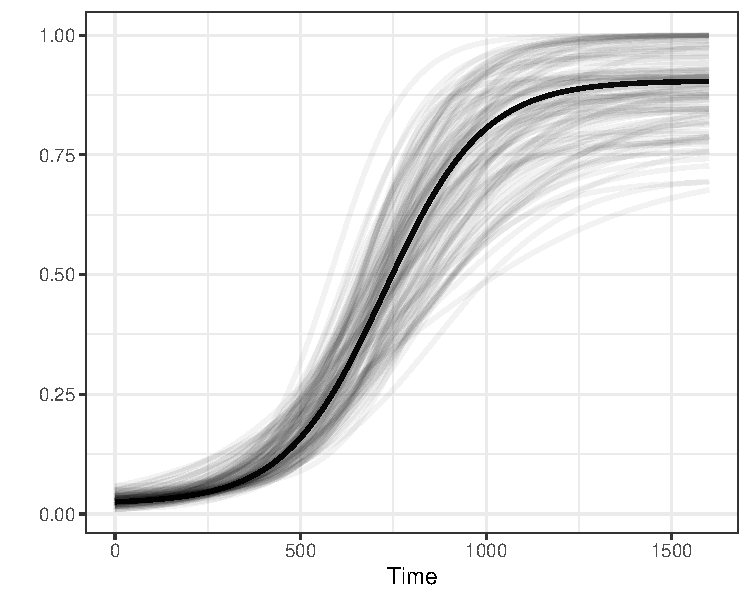
\includegraphics[width=0.45\textwidth]{logistic_distribution.pdf}} 
    \subfigure[]{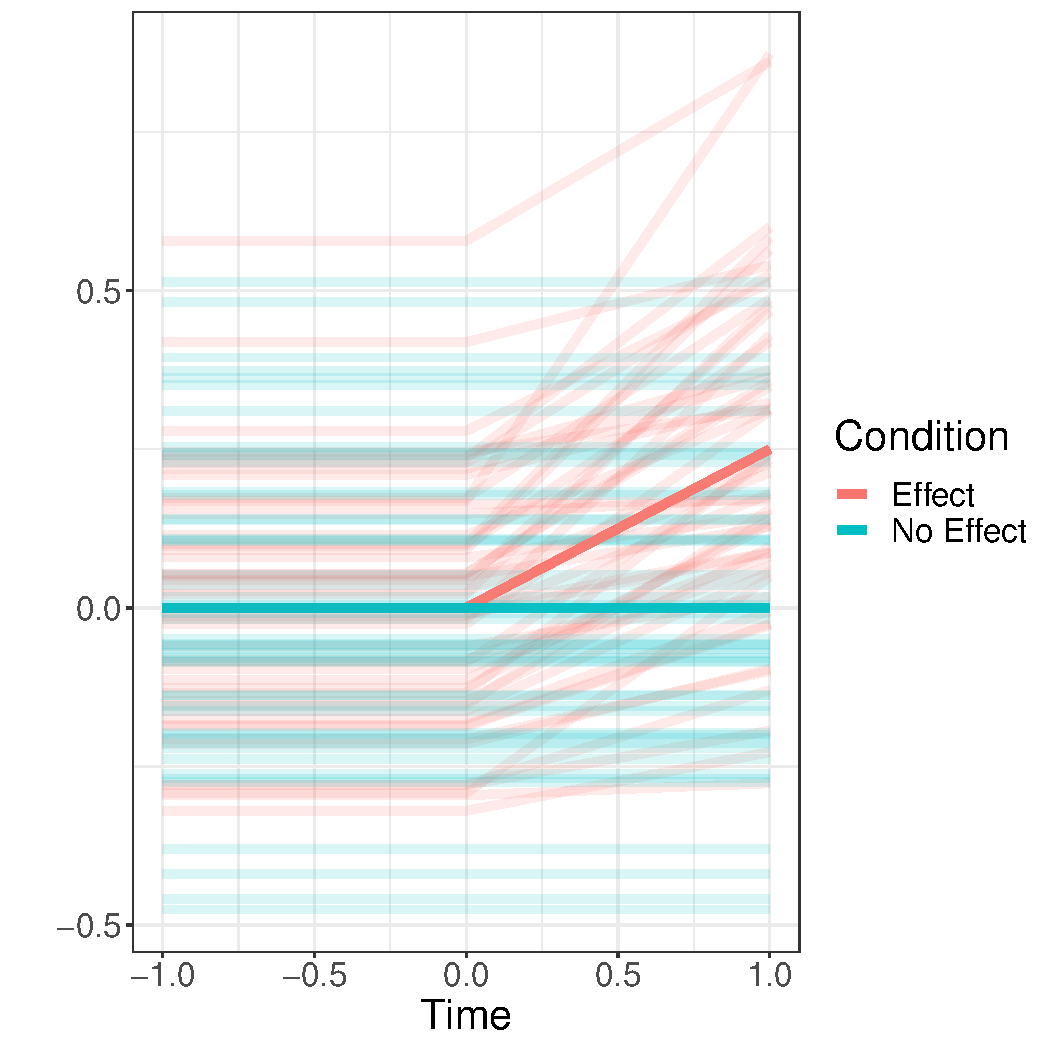
\includegraphics[width=0.45\textwidth]{piecewise_distribution.pdf}}
    \caption{Distributions of various group with the mean curve in bold (a.) 50 samples from the generating distribution of the four-parameter logistic in Equation~\ref{eq:logistic} used for testing FWER. (b.) 50 samples from the generating distributions of each group in Equation~\ref{eq:piecewise_form}. The legend makes size weird, might just explain what they are here. Also need to see if I can change size of the mean lines}
\label{fig:distribution}
\end{figure}



We further assume that each group drew subject-specific parameters from a normal distribution, with subject $i = 1, \dots, N$ in group $g = 1, \dots, G$ following the distribution in Equation~\ref{eq:theta_i_dist}.

\cn{Could also expression this $\theta_i^{(g)}$? Though that may be cumbersome}

\paragraph{Mean Structure} In all of the simulations presented, the distribution used in Equation~\ref{eq:tie_dist} was empirically determined from data on normal hearing subjects in the VWP (Farris-Trimble et  al., 2014 \cite{FarrisTrimble2014}). Parameters used were those fit to fixations on the Target, following the functional form of Equation~\ref{eq:logistic}. Under the assumption of between-subject homogeneity, we set $\theta_i = \theta_j$ for all subjects $i,j$, assuring that each of the subjects' observations is derived from the same mean structure, differing only in their observed error. We will call this the homogeneous means assumption.


\paragraph{Error Structure} The error structure is of the form

\begin{equation}
e_{it} = \phi e_{i, t-1} + w_{it}, \quad w_{it} \sim N(0, \sigma)
\end{equation}
where the $w_{it}$ are iid with $\sigma = 0.025$. $\phi$ corresponds to an autocorrelation parameter and is set to $\phi = 0.8$ when the generated data is to be autocorrelated and set to $\phi = 0$ when we assume the errors are all independent and identically distributed. 

\paragraph{Paired Data} Finally we considered paired data, though this is only a sensible condition under the assumption of heterogeneous means. In order to construct paired data, we simply used the same parameter estimates for each subject between groups, with the observed data between subjects differing only in the observed error.


Each set of conditions generates two groups, with $n = 25$ subjects in each group, with timepoints $t = 0, 4, 8, \dots, 1600$ in each trial and with $100$ simulated trials for each subject. Columns in the tables indicate homogeneity of means assumption, whether or not an AR(1) error structure was used in constructing the data, and if autocorrelation was specified in the fitting function. The last conditions helps assess the impact of correctly identifying the type of error when conducting an analysis in \xt{bdots}. Each simulation was conducted 100 times to determine the rate of type I error (time intensive and will launch 1000 for final dissertation). 


\subsection{Results}

We consider the efficacy the methods under each of the simulation settings with an analysis of the family wise error rate (FWER) and the median per-comparison error rate. The first of these details the proportion of simulations under each condition that marked \textit{at least} one time point as being significantly different between the two groups. This is critical is understanding each method's ability to correct adjust for the multiple testing problem associated with testing each of the observed time points. These are presented in Table~\ref{tab:fwer_unpaired} and Table~\ref{tab:fwer_paired} for unpaired and paired data, respectively.

Complimenting the FWER estimate is an estimate of the median per-comparison rate. For each time point across each of the simulations, we computed the proportion of times in which that time was determined significant. The median of these values across all time points is what is considered. This metric gives a sense of magnitude to the binary FWER; for example, a situation in which there was a high FWER and low median per-comparison rate would indicate that the type I error within a particular time series would be sporadic and impact limited regions. Large median per-comparison rates indicate that large swaths of a time series frequently sustain type I errors. The median per-comparison rates for unpaired and paired simulations are presented in Table~\ref{tab:mpc_unpaired} and Table~\ref{tab:mpc_paired}.


\subsubsection{FWER}



There are a few things of immediate note when considering the results of Table~\ref{tab:fwer_unpaired}. First, we see from the first two settings of the unpaired simulations that the type I error rates for the homogenous bootstrap are consistent with those presented in \cite{oleson2017detecting}, confirming the importance of specifying the existence of autocorrelation in the \xt{bdots} fitting function when autocorrelated error is present. By contrast, this is far less of a concern when using the heterogeneous bootstrap or permutation testing, both of which maintain a FWER near the nominal alpha, regardless of whether or not the error structure was correctly identified. This continues to be true under the homogenous mean assumption when the true error structure is not autocorrelated. Interestingly, the performance of the homogeneous bootstrap falters here despite theoretical consistency with the simulation settings. \cn{I am rerunning this condition again now to make sure there wasn't an error.}

The most striking results of this, however, appear when the data generation assumes a heterogeneous mean structure. While both the heterogeneous bootstrap and the permutation test maintain a FWER near the nominal alpha, the homogeneous bootstrap fails entirely, with a FWER $> 0.9$ in all cases.

\begin{table}[H]
\centering
\begin{tabular}{cccccc}
  \hline
  \multicolumn{1}{p{2cm}}{\centering Heterogeneity \\ Assumption} & \multicolumn{1}{p{2cm}}{\centering Autocorrelated \\ Error} & \multicolumn{1}{p{2cm}}{\centering AR(1)  \\ Specified} &  \multicolumn{1}{p{2cm}}{\centering Homogeneous \\ Bootstrap} &\multicolumn{1}{p{2cm}}{\centering Heterogeneous \\ Bootstrap} & \multicolumn{1}{p{2cm}}{\centering Permutation } \\ 
  \hline
No & Yes & Yes & 0.06 & 0.01 & 0.08 \\ 
  No & Yes & No & 0.87 & 0.08 & 0.00 \\ 
  No & No & Yes & 0.08 & 0.00 & 0.06 \\ 
  No & No & No & 0.15 & 0.02 & 0.01 \\ 
  Yes & Yes & Yes & 0.92 & 0.03 & 0.05 \\ 
  Yes & Yes & No & 0.96 & 0.02 & 0.08 \\ 
  Yes & No & Yes & 0.99 & 0.05 & 0.03 \\ 
  Yes & No & No & 1.00 & 0.05 & 0.06 \\  
   \hline
\end{tabular}
\caption{FWER for empirical parameters (unpaired)}
\label{tab:fwer_unpaired}
\end{table}

Paired data is given in Table~\ref{tab:fwer_paired}. Matching the conclusions drawn from Table~\ref{tab:fwer_unpaired}, we only note here that both the permutation test and heterogeneous bootstraps maintain a valid FWER under the assumption of paired data.

\begin{table}[H]
\centering
\begin{tabular}{cccccc}
  \hline
  \multicolumn{1}{p{2cm}}{\centering Heterogeneity \\ Assumption} & \multicolumn{1}{p{2cm}}{\centering Autocorrelated \\ Error} & \multicolumn{1}{p{2cm}}{\centering AR(1) \\ Specified} &  \multicolumn{1}{p{2cm}}{\centering Homogeneous \\ Bootstrap} &\multicolumn{1}{p{2cm}}{\centering Heterogeneous \\ Bootstrap} & \multicolumn{1}{p{2cm}}{\centering Permutation } \\  
  \hline
  Yes & Yes & Yes & 0.49 & 0.02 & 0.01 \\ 
  Yes & Yes & No & 0.94 & 0.03 & 0.02 \\ 
  Yes & No & Yes & 0.72 & 0.02 & 0.00 \\ 
  Yes & No & No & 0.74 & 0.04 & 0.00 \\ 
   \hline
\end{tabular}
\caption{FWER for empirical parameters (paired)}
\label{tab:fwer_paired}
\end{table}

\subsubsection{Median per comparison error rate}

We next consider the median comparison rate, which offers some insight into the FWER. In particular, consider the situation in which in Table~\ref{tab:mpc_unpaired}, in the fourth row we see a median per-comparison error rate of 0.00 for the homogeneous bootstrap, despite Table~\ref{tab:fwer_unpaired} indicating a FWER of 0.15. This is a consequence of the majority of the type I errors occuring in a relatively limited region. In contrast, the median per-comparison error rate of the homogeneous bootstrap under the assumption of heterogeneity suggests that the type I errors are widespread and not limited to any particular area. 

It is also worth commenting on the permutation test median per-comparison error rate in Table~\ref{tab:mpc_unpaired}; combined with a FWER near the nominal 0.05, these values suggest that errors are likely distributed across the entire range rather than limited to a small area (which would result in a MPCR of 0). 

\cn{I confirmed this by looking both at this histograms and inspecting the data manually}

\begin{table}[H]
\centering
\begin{tabular}{cccrrr}
  \hline
  \multicolumn{1}{p{2cm}}{\centering Heterogeneity \\ Assumption} & \multicolumn{1}{p{2cm}}{\centering Autocorrelated \\ Error} & \multicolumn{1}{p{2cm}}{\centering  AR(1) \\ Specified} &  \multicolumn{1}{p{2cm}}{\centering Homogeneous \\ Bootstrap} &\multicolumn{1}{p{2cm}}{\centering Heterogeneous \\ Bootstrap} & \multicolumn{1}{p{2cm}}{\centering Permutation } \\ 
  \hline
No & Yes & Yes & 0.01 & 0.00 & 0.04  \\ 
  No & Yes & No & 0.31 & 0.00 & 0.04 \\ 
  No & No & Yes & 0.00 & 0.00 & 0.02\\ 
  No & No & No & 0.00 & 0.00 & 0.03 \\ 
  Yes & Yes & Yes & 0.51 & 0.01 & 0.01 \\ 
  Yes & Yes & No & 0.76 & 0.01 & 0.00 \\ 
  Yes & No & Yes & 0.86 & 0.01 & 0.00 \\ 
  Yes & No & No & 0.81 & 0.01 & 0.00 \\ 
   \hline
\end{tabular}
\caption{median per comparison error rate (unpaired)}
\label{tab:mpc_unpaired}
\end{table}



\begin{table}[H]
\centering
\begin{tabular}{cccrrr}
  \hline
  \multicolumn{1}{p{2cm}}{\centering Heterogeneity \\ Assumption} & \multicolumn{1}{p{2cm}}{\centering Autocorrelated \\ Error} & \multicolumn{1}{p{2cm}}{\centering AR(1) \\ Specified} &  \multicolumn{1}{p{2cm}}{\centering Homogeneous \\ Bootstrap} &\multicolumn{1}{p{2cm}}{\centering Heterogeneous \\ Bootstrap} & \multicolumn{1}{p{2cm}}{\centering Permutation } \\ 
  \hline
  Yes & Yes & Yes & 0.13 & 0.00 & 0.00 \\ 
  Yes & Yes & No & 0.52 & 0.02 & 0.00 \\ 
  Yes & No & Yes & 0.38 & 0.01 & 0.00 \\ 
  Yes & No & No & 0.44 & 0.01 & 0.00 \\ 
   \hline
\end{tabular}
\caption{median per comparison error rate (paired)}
\label{tab:mpc_paired}
\end{table}


\subsection{Discussion}

Table~\ref{tab:fwer_unpaired} and Table~\ref{tab:fwer_paired} demonstrate that under a variety of settings, both the heterogeneous bootstrap and permutation offer a FWER near the nominal alpha, making their performance similar to that of the homogeneous bootstrap in the best of cases. This includes less restrictive assumptions in which they continue to perform well while the homogeneous bootstrap maintains an unacceptably high FWER. 

Transition sentence to power simulations

\section{Power Simulations}


To determine power, two experimental groups were simulated with mean structures of the following form:

\begin{equation}\label{eq:piecewise_form}
y = \begin{cases}
b \quad &x < 0 \\
mx + b \quad &x \geq 0
\end{cases}
\end{equation}

The first simulated group was ``No Effect", with intercept and slope parameters normally distributed and standard deviation $\sigma = 0.05$. The second group, the ``Effect" group, was similarly distributed, but with the slope parameter having mean value of $\mu = 0.25$. The error structure was identical to that in the FWER simulations, with both an AR(1) error structure and independent noise included. 100 simulations were conducted for each scenario. 

We limited consideration to three possible scenarios: first, we assumed the conditions presented in Oleson 2017, assuming homogeneity between subject parameters and an AR(1) error structure, with the model fitting performed assuming autocorrelated errors. For the remaining scenarios, we assumed heterogeneity in the distribution of subject parameters, simulated with and without an AR(1) error structure. In both of these last two scenarios, we elected to \textit{not} fit the model assuming autocorrelated errors. This was for two reasons: first, simulations exploring the type I error rate suggested that models fit with the autocorrelation assumption tended to be conservative. Second, and given the results of the first, this makes setting the assumption of autocorrelation to FALSE in \xt{bdots} seem like a sensible default, and as such, it would be of interest to see how the model performs in cases in which their is autocorrelated error that is not accounted for.

For each subject, parameters for their mean structure given in Equation~\ref{eq:piecewise_form} were drawn according to their group membership and fit using \xt{bdots} on the interval (-1,1). Time windows in which the groups differed were identified using each the homogenous bootstrap, heterogeneous bootstrap, and permutation testing. By including the interval (-1,0) in which the null hypothesis was true, we are able to mitigate the effects of over-zealous methods in determining power, and we present the results in the following way: any tests in which a difference was detected in (-1,0) was marked as having a type I error, and the proportion of simulations in which this occurred for each method is reported as the FWER in the column labeled $\alpha$. The next column, $\beta$, is the type II error rate, indicating the proportion of trials in which no differences were identified over the entire region. The last Greek-letter column is $1 - \beta - \alpha$, a modified power statistic indicating the proportion of tests in which a difference was correctly identified. The remaining columns relate to this modified power columns, giving a partial summary of the earliest onset of detection. As a true difference occurs on the interval $t > 0$, smaller values indicate greater power in detecting differences. Finally, a (currently base-R) plot giving the power at each time point is given in Figure~\ref{fig:time_power_plot}. This plot represents the true power, though note that it does not take into account the rate at which these regions were identified in conjunction with a type I error rate.



\subsection{Results}

The results of the power simulation are presented in Table~\ref{tab:power_methods}. We begin by considering the case in which we assumed a homogeneous mean structure with autocorrelated errors (the first three rows), matching the conditions in which the homogeneous bootstrap was first presented. Notably, we find that the permutation method demonstrates the greater power, with the median onset time just under that of the homogeneous bootstrap. This is at the expense of a larger FWER, though still below the nominal level. Alternatively, the heterogeneous bootstrap maintains a similar FWER as the homogeneous bootstrap at the cost of power.

The remaining settings tell a similar story with the exception of the homogeneous bootstrap which continues to demonstrate unacceptable FWER under the heterogeneous means assumption. We also seem some effect of not correctly specifying an AR(1) error structure when comparing the last two settings, as the failure to specify resulted in a slightly higher FWER and lower power, although not significantly (it may be worth it to include setting with AR(1) error correctly specified to see how it compares). 


% latex table generated in R 4.2.2 by xtable 1.8-4 package
% Sat Feb 18 14:03:58 2023
\begin{table}[H]
\centering
\begin{tabular}{lcccccccc}
  \hline
Method & Heterogeneity & AR(1) & $\alpha$ & $\beta$ & 1 - $\alpha$ - $\beta$ & 1st Qu. & Median & 3rd Qu. \\ 
  \hline
Hom. Boot & No & Yes & 0.00 & 0.00 & 1.00 & 0.025 & 0.030 & 0.035 \\ 
  Het. Boot & No & Yes & 0.00 & 0.00 & 1.00 & 0.035 & 0.040 & 0.045 \\ 
  Perm & No & Yes & 0.03 & 0.00 & 0.97 & 0.015 & 0.025 & 0.025 \\ 
  \hline
  Hom. Boot & Yes & No & 0.96 & 0.00 & 0.04 & 0.005 & 0.008 & 0.010 \\ 
  Het. Boot & Yes & No & 0.00 & 0.10 & 0.90 & 0.403 & 0.513 & 0.690 \\ 
  Perm & Yes & No & 0.03 & 0.05 & 0.92 & 0.378 & 0.515 & 0.681 \\ 
  \hline
  Hom. Boot & Yes & Yes & 0.97 & 0.00 & 0.03 & 0.008 & 0.010 & 0.010 \\ 
  Het. Boot & Yes & Yes & 0.01 & 0.10 & 0.89 & 0.420 & 0.525 & 0.690 \\ 
  Perm & Yes & Yes & 0.08 & 0.03 & 0.89 & 0.360 & 0.540 & 0.705 \\ 
   \hline
\end{tabular}
\caption{Power for methods (possibly include AR(1) error and AR(1) specification to compare to last setting)} 
\label{tab:power_methods}
\end{table}

The results in Table~\ref{tab:type_2_summary} are a summary of all of the methods found by taking the mean of each of the results presented. This is intended to interrogate the performance of each of these methods when underlying assumptions are unknown or unspecified. We find a robust performance for each of the new methods presented, maintaining a reasonable relationship between FWER and power. The metrics associated with homogeneous bootstrap are perhaps a bit misleading here as they appear to demonstrate exceptional power, though at the cost of unacceptable type I error.

% latex table generated in R 4.2.2 by xtable 1.8-4 package
% Sat Feb 18 14:11:04 2023
\begin{table}[ht]
\centering
\begin{tabular}{lcccccc}
  \hline
Method & $\alpha$ & $\beta$ & $1 - \alpha - \beta$ & 1st Qu. & Median & 3rd Qu. \\ 
  \hline
Hom. Bootstrap & 0.643 & 0.000 & 0.357 & 0.013 & 0.016 & 0.018 \\ 
  Het. Bootstrap & 0.003 & 0.067 & 0.930 & 0.286 & 0.359 & 0.475 \\ 
  Permtuation & 0.047 & 0.027 & 0.927 & 0.251 & 0.360 & 0.470 \\ 
   \hline
\end{tabular}
\caption{Summary of methods for Type II error} 
\label{tab:type_2_summary}
\end{table}

\subsubsection{Summary of methods}



\begin{figure}[H]
\centering.
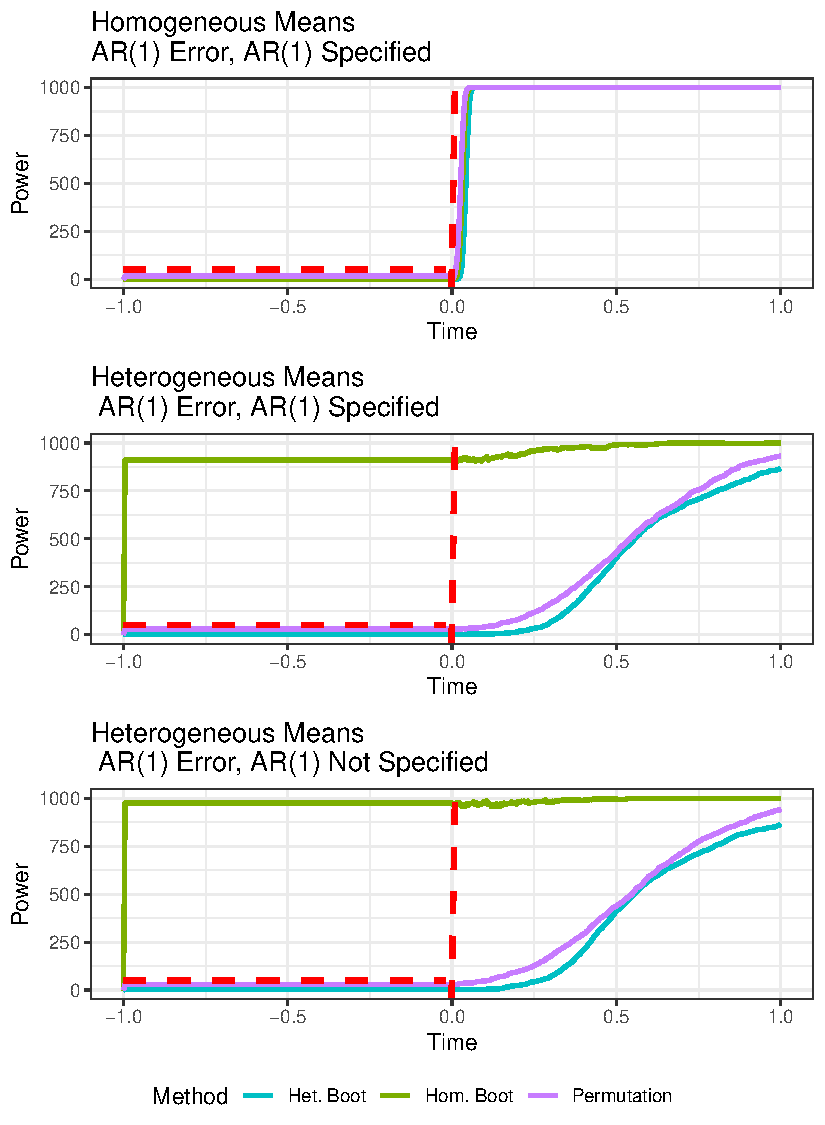
\includegraphics{typeII_time.pdf}
\caption{Observed power of each of the methods at each time in (-1,1) (not sure if better as subplots?)}
\label{fig:time_power_plot}
\end{figure}

%\begin{figure}[H]
%\centering
%    \subfigure[]{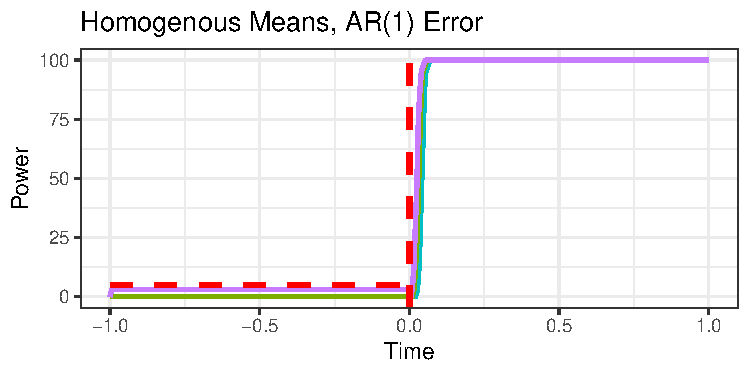
\includegraphics{type_two_error_time_a.pdf}}
%    \subfigure[]{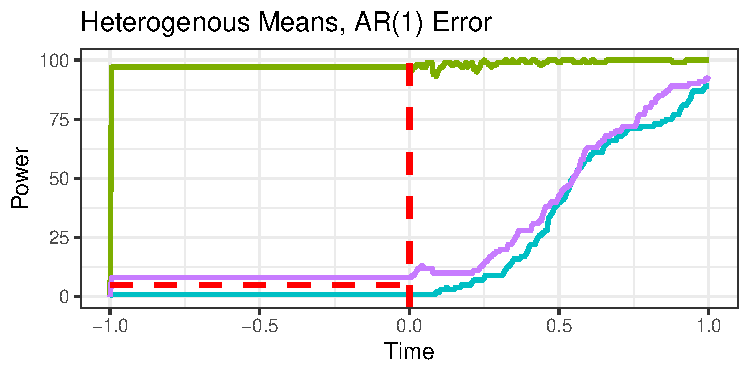
\includegraphics{type_two_error_time_b.pdf}}
%        \subfigure[]{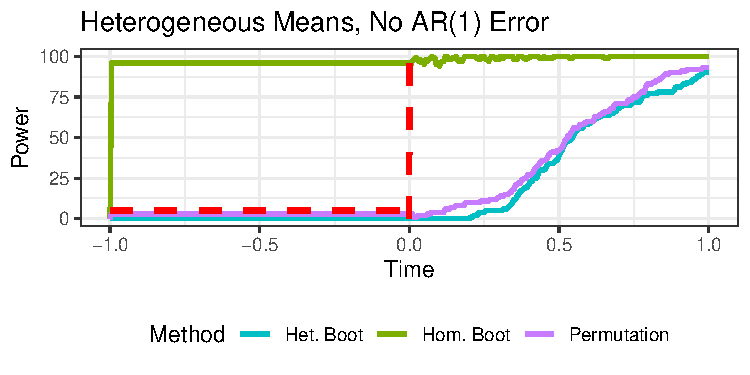
\includegraphics{type_two_error_time_c.pdf}}
%\caption{Observed power of each of the methods at each time in (-1,1)}
%\label{fig:time_power_plot}
%\end{figure}

\section{Discussion and concluding remarks}

We set out both to interrogate the validity of the homogenous bootstrap assumptions and to propose two alternative methods that would be more robust under a greater variety of assumptions. In doing so, we demonstrated conclusively the utility of the heterogeneous bootstrap and permutation tests while also highlighting a major shortcoming of the original. It's worth noting, however, that the FWER adjustment proposed in \cite{oleson2017detecting} is still valid, if not slightly conservative, and with power similar to that of the permutation method. 

In light of the results presented, one issue of concern is addressing the fact that a version of \xt{bdots} with the homogeneous mean assumption was presented in 2018 and remained accessible on CRAN until the end of 2022. This has implications for the number of papers in which \xt{bdots} may have demonstrated significance between groups when the underlying assumptions of homogeneous mean structure did not hold, as is likely the case in all instances related to the VWP. Concurrent with this issue is the issue of identifying current users of \xt{bdots} of this change, as results found only a month ago will be profoundly different than what is seen today. At present, I am not sure the best way to address either of these. In either case, however, it will be prudent to remove this option from the \xt{bdots} package all together, as there appears to be no obvious advantage to the homogeneous bootstrap over the others in terms of either controlling the FWER or obtaining power, even when the homogeneous mean structure assumption is met.

There are several limitations of the current paper that are worthy of further investigation. First, First, limited consideration was given to the effect of sample density on the observed type I error rate or power. As the fitting function in \xt{bdots} simply returns a set of parameters, one could conceivably perform any of the methods presented on any arbitrary collection of points, whether or not any data were observed there. This extends itself to the condition in which subjects were sampled at heterogeneous time points, as may be the case in many clinical settings. What impact this may have or how to best handle these cases remains open for exploration. It is also worth investigating in greater detail what impact the re-drawing of subject specific parameters from their respective distributions has on both the FWER and power, as in several of the simulations the observed FWER was much lower than the nominal level. Particularly in the case of the permutation method which is \textit{not} seeking to estimate the group distributions, it may be worthwhile to see if a favorable trade can be made to increase the resulting power.

We conclude by noting that \xt{bdots} is now equipped with two methods to effectively control the FWER when assessing the differences in time series under a greater set of underlying assumptions, including those involving the presence of highly correlated test statistics. Further, both methods presented are robust to misspecification of the error structure while maintaining an acceptable FWER and adequate power. 




\bibliography{../bib/dissertation}

\end{document}








\begin{abstract}
The Bootstrapped Differences of Timeseries (bdots) was first introduced by Oleson (and others) as a method for controlling type I error in a composite of serially correlated tests of differences between two time series curves in the context of eye tracking data.  This methodology was originally implemented in R by Seedorff 2018. Here, we revist the original package, both improving the underlying theoretical components and creating a more robust implementation.
\end{abstract}

\section{Introduction}

In 2017, Oleson et al. introduced a method for detecting time-specific differences in densley sampled time series. This largely centered around bootstrapping and computing a series of highly correlated $t$-statistics and using estimates of the autocorrelation as an adjustment for the family-wise error rate. This paper was presented in the context of the Visual World Paradigm (VWP), an experimental paradigm combining eyetracking with an interactive environment to measure dynamics in language processing, and in 2018, R software was introdued on CRAN to perform a limited version of the analysis proposed in Oleson. In this paper, we introduce \texttt{bdots} v2, an update to the CRAN package that broadly expands the capabilities of the original. 

This paper is not intended to serve as a complete use guide to updates in the bdots package. Rather, the purpose is to showcase major changes and improvements to the package, with those seeking a more comprehensive treatment directed to the package vignettes. Updates to the bdots package have been such that there is little resemblance to the original. Rather than taking a ``compare and contrast" approach, we will first enumerate the major changes, followed by a general demonstration of the package use. 

\begin{enumerate}
\item Simplified user interface
%\item Parameter and nonparametric functions (not going to be true)
\item User defined curves
\item Permit fitting for arbitrary number of groups
\item Updates to bootstrapping algorithm and introduction of permutation test
\item Automatic detection of paired tests based on subject identifier
\item Allows for non-homogenous sampling of data across subjects and groups
\item Introduce formula syntax for bootstrapping difference function
%\item Removal of auto-correlation assumption
\item bdots object inherits from data.table class
\item bdots is now stylized ``bdots"
\end{enumerate}

\paragraph{Bootstrapped differences in time series}

The high level motivation, abstracted from the particulars, is more or less as follows: we are often interested in comparing time series between two or more groups. A full(er) review of previous methods can be found in Seedorff,  though we can limit the scope of interest to specifying that we are interested in ``developing a statistical tool to (1) detect differences in two time series (as the VWP) and (2) to offer a precise characterization of the time window in which a difference occurs \cite{seedorff2018bdots}."

A typical instantiation of this problem occurs when we have two groups (or experimental conditions, etc.,) in which subjects in each group have an associated time series. It's assumed that each group has some distribution of associated functions in time, and we are interested in identifying windows in time in which these distributions are significantly different.


[Not sure if we include this here ]There are also situations in which we are interested in the difference of differences. I don't remember where or why this is done, some justification for doing this instead of some complicated F test, but I can find that later. Instead, let me offer an example. I'm already not going to like this example, so let me just put it anyways knowing that it will be deleted. Suppose we are interested in understanding how the color of a vehicle differentially impacts performance based on the vehicle type. We know that there is some difference between cars and trucks. Suppose then that we look at the difference between red cars and red trucks and then the difference between blue cars and blue trucks. If color does not mediate this difference, the difference between red cars and trucks should be the same as the difference between blue cars and trucks. This information can be determined if we look then at the difference between the differences. 

The original bdots package was predicated on comparing differences between dense, highly correlated time series by first specifying functional forms and then performing statistical tests on each of the observed time points. With verison 2.0, capabilities have drastically improved, and bdots is able to fit parameteric functions to any type of data observed in time. Along with methodological improvements, we have included more options in determining statistical significance in the differences of curves, utilizing a robust permutation testing framework when the assumptions of autocorrelation do not hold. In addition to methodology, a number of quality-of-life improvements have also been made, greatly simplifying syntax, creating more robust functions, and including a collection of useful methods for handling returned objects.

In summary, \texttt{bdots} has transitioned from a package focused exclusively on densly sampled timeseries assuming a limited number of functional forms to a robust framework for identifying time windows of significant difference across a wide breadth of timeseries-adjacent data. 

%talk about how we are no longer just doing time series, as indicated with saccade method. we have now branched to the more general problem of comparing functional forms of observed data.

\section{Methodology and Overview} 

There are major changes in the underlying methodology used in the bdots package, and we will briefly review the current methodology here (without explicit comparisons to the original). For those interested, please see some other article that I have to write.

Broadly, there are two steps to performing an analysis with the \xt{bdots} package: fitting the curves to observed data and bootstrapping differences between groups. The first step involves specifying an underlying curve $f$, which is assumed to be parametric\footnote{the option to include non-parametric functions is anticipated in the future work of this package. The process will be similar, however, with $\theta$ then representing the number and location of the knots for splines}. Along with the observed data $y$ for each $i$th subject, \xt{bdots}, via fitting with \xt{gnls}, returns a set of parameters along with an estimate of their covariance.

\begin{equation}
F: f \times y_i \rightarrow N(\hat{\theta_i}, V_{i}),
\end{equation}
where $\theta$ is a length-$p$ vector representing the parameters of the function.


Once fits have been made, we are ready for testing the bootstrapped difference between curves. After specifying the groups of interest for analysis, two algorithms are implemented: a bootstrapping algorithm is used to determine the distribution of each group of curves, while either permutation testing or bootstrapping is used to specify regions of statistically significant differences, depending on the underlying assumptoins made. The algorithm for  bootstrapping for each group is as follows:

\begin{enumerate}
\item For a group of size $n$, select $n$ subjects from the group, \textit{with replacement}
\item For each selected subject, draw a set of parameters from the distribution $\theta_{i}^* \sim N(\hat{\theta}_i, V_i)$. This permits us to account for within subject variability
\item For each of the resampled $\theta_i^*$, find the $b$th bootstrap estimate for the group $\theta_b = \frac1n \sum_{i=1}^n \theta_i^*$
\item Perform this sequence $B$ times
\end{enumerate}


The end results is a $B \times p$ matrix containing a bootstrapped sample of the group distribution for $\theta$. Each row of this matrix is used to create a $1 \times T$ vector representing $f_{\theta}$ evaluted at $T$ time points. This results in a $B \times T$ matrix representing a collection of bootstrapped curves evaluated at each time point, in total representing a bootstrapped distribution of the curves.


%Each of these is used to construct a $B \times T$ matrix ($T$ the number of time points), a collection of bootstrapped curves. Each column of this matrix represents a time point, $t$, from which we can compute the mean and standard deviation of the group curve at that time (wordy). $\Leftarrow$ this also might contain too specific of detail. they don't care that its a matrix. they care for each time point we can construct an estimate of the mean and sd. And really, even this is only from CI and group distribution. There could possibly be an option to skip computing this at all and just do the permutation test.

Next we attend to idenfiying regions in which a statistically significant difference between curves is present, choosing from one of the two methods currently available.

\subsection{Permutation Testing}

The simplest method implemented for idenfiying time-specific differences is permutation testing, ideal when minimal assumptions can be made on the observed data. 

We begin by computing a $t$-statistic of the difference at each time point, 

\begin{equation}
T(t) = \frac{|\overline{f}_1(t) - \overline{f}_2(t)|}{\sqrt{\frac{1}{n_2} \text{Var}(f_1(t)) + \frac{1}{n_2} \text{Var}(f_2(t))}}, \quad \Leftarrow \text{ check these (specifically n in denom)}
\end{equation}
or, in the case of paired groups, 

\begin{equation}
T(t) = \frac{\overline{f}_D(t)}{\sqrt{\frac1n \text{Var}(f_D(t))}}.
\end{equation}

Next, we go about creating a null distribution against which to test our hypothesis that there is no difference between each group at each time point. We do this with permutation testing, and the algorithm is as follows: for two groups, with $n_1$ and $n_2$ subjects in each

\begin{enumerate}
	\item Assign to each subject a label indicating group membership
	\item Randomly shuffle the lables indicating membership, creating two new groups with $n_1$ and $n_2$ subjects in each
	\item Recalculate the $t$-statistic, $T(t)$ and log the maximum
\end{enumerate}

The collection of maximum values for $T(t)$ will serve as the null distribution against which to compare our observed $T(t)$. Regions in which the observed $t$ statistic are beyond the specified $\alpha$ in the null distribution are then considered significant.

This notation was clearly stolen from the FDA book. 

\subsection{FWER Adjustment}

In addition to permutation testing, there are also adjustments that can be made to control for the family-wise error rate. As was done with permutation testing, we begin by computing a $t$-statistic at each time point for the observed data, 

\begin{equation}
T(t) = \frac{|\overline{f}_1(t) - \overline{f}_2(t)|}{\sqrt{\frac{1}{n_2} \text{Var}(f_1(t)) + \frac{1}{n_2} \text{Var}(f_2(t))}}, \quad \Leftarrow \text{ check these (specifically n in denom)}
\end{equation}
or, again in the case of paired groups, 

\begin{equation}
T(t) = \frac{\overline{f}_D(t)}{\sqrt{\frac1n \text{Var}(f_D(t))}}.
\end{equation}

Unlike the case with the permuted data, we have no need for a null distribution, instead determining significance by considering the observed statistics against a modified $\alpha$.  Adjustments that can be made include all of the adjustments found in \xt{stats::p.adjust}, and adjustment made on the false discovery rate (FDR), and finally the adjustment ``oleson" used in the original \xt{bdots} package. In short, the ``oleson" adjustment makes use of an autocorrelation parameter to adjust for the highly correlated series of $t$-statistics. A full treatment of this methodology is included in Oleson 2017.

---

[doesn't really need to be included] In addition to whatever general uncertainy exists in the section above, we again now need to consider if we want each iteration of our bootstrap to be $f ( \frac1n \sum \theta_{bi})$ or $ \frac1n \sum f_i (\theta_{bi})$

\section{Example Data}

We will illustrate use of the updated \xt{bdots} package with a worked example, using an artificial dataset to help detail some of the newer aspects of the package. The dataset will consist of outcomes for a collection of vehicles, consisting of eight distinct groups. These groups will be nested in order of vehicle origin (foreign or domesetic), vehicle class (car or truck), and vehicle color (red or blue). Further, vehicles of different color but within the same origin and class groups will be considered paired observations. A table detailing the relationship of the groups is shown here:

\begin{center}

\begin{tabular}{|p{0.9in}|p{0.9in}|p{0.9in}|} \hline 
\rowcolor{lightgray} \multicolumn{1}{|c|}{Origin} & \multicolumn{1}{c|}{Class} & \multicolumn{1}{c|}{Color}\\
\hline
\multirow{4}{*}{foreign} & \multirow{2}{*}{car} & red \\
\hhline{~~-}
& & blue \\
\hhline{~--}
& \multirow{2}{*}{truck} & red \\
\hhline{~~-}
& & blue \\
\hline
\multirow{4}{*}{domestic} & \multirow{2}{*}{car} & red \\
\hhline{~~-}
& & blue \\
\hhline{~--}
& \multirow{2}{*}{truck} & red \\
\hhline{~~-}
& & blue \\
\hline
\end{tabular}
\end{center}

The outcome here is simply \xt{y} due to a lack of creativity, but the functional form assumed (and used in data generation) follows the four parameter logistic, 

\begin{equation}
f_{\theta}(t) = b + \frac{p-b}{1 + \exp \left( \frac{4s}{p-b} (c-t \right)},
\end{equation}
where $b$, $p$, $s$, and $c$ represent the baseline, peak, slope, and crossover points, respectively


\section{Fitting Curves}

The curve fitting process is performed with the \texttt{bfit} function (previously \texttt{bdotsFit}), taking the following arguments: (removing `cor` and numRefits)

\begin{center}
\begin{verbatim}
bfit(data, subject, time, y, group, curveType, cores, ...)
\end{verbatim}
\end{center}

\paragraph{Curve functions} Each of \texttt{subject}, \texttt{time}, and \texttt{y}, are length one character vectors representing columns of the dataset used in \texttt{data}, while \xt{group} is a character vector (of varying length), also column(s) found in \xt{data}. New here is \texttt{curveType}, taking as an argument an R call to a particular curve, for example the four parameter logistic, \texttt{bdots::logistic()}. This is done to self-contain any additional arguments associated with the fitting curve, for example the concavity of the double-Gaussian (\texttt{curveType = doubleGauss(concave = TRUE)}) or the number of degrees in a polynomial (\texttt{curveType = polynomial(degree = 5)}). A number of curves are included with the \texttt{bdots} package, including those for the four-parameter logistic, the double-Gaussian, an exponential curve, and polynomials of arbitrary degree. A detailed vignette on writing custom curves can be found with \texttt{vignette("bdots")} ($\Leftarrow$ actually it would be vignette(``customCurves", "bdots") or browseVignette(``bdots") to see, but I haven't decided which I want because I don't really like the name customCurves).

Notably, \texttt{bdots} can now fit curves to an arbitrary number of groups at once, so long as all have the same parametric specification. Fitting a collection of curves to our vehicle data with all of the groups with the logistic function would look like


\begin{center}
\begin{verbatim}
# Need to change these once I get real data
fit <- bfit(data = Vehicle, subject = "vehicle", 
	 	time = "Time", y = "out", group = c("origin", "class", "color"),
	 			curveType = logistic(), cores, ...).
\end{verbatim}
\end{center}


\paragraph{Return object and generics}



The function \texttt{bfit} returns an object of class \texttt{bdotsObj}, inheriting from class \texttt{data.table}. As such, each row of this object (object object object i need a new word) uniquely identifies one permutation of subject group (meaning if a subject in two groups, they get two rows). Included in this row are the subject identifier, group classification, summary statistics regarding the curves, and a nested gnls object. Not sure if this is worth including, most people won't use it and i can put it in the vignette.


Several methods exist for this object, including \texttt{plot}, \texttt{summary}, and \texttt{coef}, returning a matrix of fitted coefficients returned from \texttt{gnls}. One consequence of inheriting from \texttt{data.table}, we are able to utilize data.table syntax. Note, for example, the differences between \texttt{coef(fit)}, \texttt{coef(fit[group == "A",])}, and \texttt{coef(fit[group == "B",])}. That's pretty much it on the neat stuff you can do with this. Time to go to bootstrapping step.

Actually, there is one additional thing here that I might include as an aside for now -- for part 2 of disseration, we are fitting curve to saccades instead of an ``observed" function. In this case, $R^2$ ends up being kind of a dumb/silly metric. Same can be said for auto-correlation (in terms of it being relevant). Both of these things are included in the derivation of the \texttt{fitCode}. Have not yet decided how that will be handled. 

\paragraph{Fit Codes}

need to decide what i'm going to do about this. would be nice if the metric used here was module, and it can be, just not right now because that would be a lot of extra work for nothing. I could just ignore this issue all togtetrher, indicate that this is for correlation and R2, and made absolutely no mention of how this possibly conflicts with other types of data

\section{Bootstrapping}

Like the fitting function, the bootstrapping process has been consolidated to a single function, \texttt{bboot} (previously \texttt{bdotsBoot}). As we will detail, the number of options included in the \xt{bboot} function have expanded considerably. A call to \xt{bboot} takes the following form

\begin{center}
\tt bboot(formula, bdObj, Niter, alpha,   padj = "oleson", \\ cores = 0, permutation = FALSE, ...)
\end{center}

By default, significance is determined with an adjustment to the family-wise error rate, as was done in the original implementation of \xt{bdots}, using method \xt{padj = "oleson"}. When setting the argument \xt{permutation = TRUE}, \xt{padj} is ignored and permutation testing for regions of difference is used instead (bootstrapping is still used for determining the group distribution, however).

A key component of the bootstrapping function is specifying which groups in our dataset we are wishing to analyze and how. This is done with a formula syntax unique to \xt{bdots} explained in the next section.

\subsection{Formula}


The formula argument serves two functions in \xt{bboot}: first, it specifies the collection of curves we wish to investigate the difference between, and second, it determines if we are interested in directly comparing the differences or the difference of differences between curves. 

To begin, let's reintroduce the structure of the groups we have in our dataset. Recall that we have foreign and domestic cars and trucks, and each of these vehicles comes in red and blue. Recall also that the different colors of each vehicle are considered paired observations.

%\begin{center}
%\begin{tabular}{|p{0.6in}|p{0.3in}|p{0.9in}|p{0.9in}|p{0.8in}|} \hline 
%\multicolumn{2}{|c|}{\multirow{2}{*}{$P_\mathrm{batt}$}} &                                                   
%  \multicolumn{3}{|c|}{$P_\mathrm{mot}$ }  \\ \cline{3-5} 
%\multicolumn{2}{|c|}{}   & S & M & H \\ \cline{1-5} 
%\multirow{3}{*}{SOC} & S & S & Z & VS \\ \cline{2-5} 
% & M & M & Z & H \\ \cline{2-5} 
% & H & M & Z & H \\ \hline 
%\end{tabular}
%\end{center}

\begin{center}

\begin{tabular}{|p{0.9in}|p{0.9in}|p{0.9in}|} \hline 
\rowcolor{lightgray} \multicolumn{1}{|c|}{Origin} & \multicolumn{1}{c|}{Class} & \multicolumn{1}{c|}{Color}\\
\hline
\multirow{4}{*}{foreign} & \multirow{2}{*}{car} & red \\
\hhline{~~-}
& & blue \\
\hhline{~--}
& \multirow{2}{*}{truck} & red \\
\hhline{~~-}
& & blue \\
\hline
\multirow{4}{*}{domestic} & \multirow{2}{*}{car} & red \\
\hhline{~~-}
& & blue \\
\hhline{~--}
& \multirow{2}{*}{truck} & red \\
\hhline{~~-}
& & blue \\
\hline
\end{tabular}
\end{center}

Let's begin with a simple case: supposing we want to investigate the difference in outcome between foreign and domestic cars. Notionally, we would write

\begin{center}
\tt y $\sim$ Origin(foreign, domestic).
\end{center}

Note that this involves the grouping variable, \xt{Origin}, with the two values we are interested in comparing, \xt{domestic} and \xt{foreign}. With this specification, the distribution of functions considered in \xt{domestic} include all red and blue domestic cars and trucks.


If we wanted to limit our investigation to only foreign and domestic cars, we would do this by including an extra term specifying the group and the desired value. In this case, 

\begin{center}
\tt y $\sim$ Origin(foreign, domestic) + Class(car).
\end{center}
To compare only foreign and domestic \textit{red} cars, we would add an additional term for color:

\begin{center}
\tt y $\sim$ Origin(foreign, domestic) + Class(car) + Color(red).
\end{center}



In each of these cases, we have specifed particular groups or nesting of groups who's outcomes we wish to compare. Alternatively, we may be interested in comparing the \textit{difference of differences}. For example, suppose we suspect that there may be some difference between red and blue vehicles, and that this difference may be different for cars compared to trucks. Whereas previously we were interested in comparing the differences in \xt{y} between groups, we are now interested in comparing the differences of \xt{y} between colors. Consequently, we will include this difference on the left hand side of the formula. This is done using \xt{diffs} syntax as such:

\begin{center}
\tt diffs(y, Color(red, blue)) $\sim$ Class(car, truck)
\end{center}

Similar as to the case before, if we wanted to limit this difference of differences investigation to only include domestic vehicles, we can do so by including an additional term:

\begin{center}
\tt diffs(y, Color(red, blue)) $\sim$ Class(car, truck) + Origin(domestic).
\end{center}

The formula syntax was originally contrived to make comparisons within groups or within nested groups. Conceivably, however, one could be interested in making the comparison between domestic red trucks and foreign blue cars. Doing so requires a bit of a work around. [what follows is my proposal that has not yet been implemented]

First, there would be some function of sorts, something like \xt{makeUniqueGroups} which would create a new group column with each permutation of previous groups being given a unique identifier. Doing this on the vehicle example would look something like \xt{fit <- makeuniquewhatever} resulting in the following grouping structure (for example) (and maybe you could specify group name and values who knows, kinda like factor this is just a working thought example)

\begin{center}

\begin{tabular}{|p{0.9in}|p{0.9in}|p{0.9in}|p{0.5in}|} \hline 
\rowcolor{lightgray} \multicolumn{1}{|c|}{Origin} & \multicolumn{1}{c|}{Class} & \multicolumn{1}{c|}{Color} & \multicolumn{1}{c|}{bgroup}\\
\hline
\multirow{4}{*}{foreign} & \multirow{2}{*}{car} & red & A\\
\hhline{~~--}
& & blue & B \\
\hhline{~---}
& \multirow{2}{*}{truck} & red & C\\
\hhline{~~--}
& & blue & D\\
\hline
\multirow{4}{*}{domestic} & \multirow{2}{*}{car} & red & E \\
\hhline{~~--}
& & blue & F\\
\hhline{~---}
& \multirow{2}{*}{truck} & red & G\\
\hhline{~~--}
& & blue & H\\
\hline
\end{tabular}
\end{center}

To then investigate differences in outcome between a foreign red car and a domestic blue truck would simply then be

\begin{center}
\tt y $\sim$ bgroup(A, H)
\end{center}

yeah not like sexy or anything but whatever it would work.

\subsection{Bootstrapping and Permutation}

Do I need this whole section again? Tie it in with the rest

Once we have determined the groups we are interested in comparing, we are ready to call the \xt{bboot} function. As detailed earlier, \xt{bboot} is now able to perform permutation testing on curve differences in addition to bootstrapping. We will discuss each of these briefly in more detail.

\paragraph{Bootstrapping} As in the original iteration of the package, \xt{bdots} seeks to identify differences in curves without a priori specification of a time window. This is done as in (other paper), where curves are bootstrapped to create a sampling distribution, and a collection of $t$-tests is performed at  each observed timepoint. The FWER is controlled against this series of tests by making an adjustment to the nominal $\alpha$ -- the novel contribution of the original \xt{bdots} package was implementing a correction based on an estimate of the autocorrelation of tests (oleson paper). In addition to this adjustment, \xt{bdots} also allows corrections to be made using a number of other methods, including fdr, bonferonni, and I think maybe another. The type of correction made is specified with the \xt{padj} argument in \xt{bboot}.

\paragraph{Permutation} In addition to the bootstrapping algorithm just described, 
\xt{bdots} now also includes the option for running a permutation test to establish a null distribution on the differences between curves. This is done by setting the argument in \xt{bboot(..., permutation = TRUE)}.  \xt{Niter} now refers to the number of permutations performed rather than the number of bootstraps. Additionally, when \xt{permutation = TRUE} is set, the argument to \xt{padj} is ignored. Permutation testing may have less power in some cases (explored in other paper), but is maximally robust and ideal for situations in which the number of assumptions made is limited.

\subsection{Summary and Analysis}

Let's begin first by running \xt{bboot} using bootstrapping to compare the outcome between  domestic cars and trucks

\begin{center}
\tt boot <- bboot(y $\sim$ Vehicle(car, truck) + Origin(domestic), fit)
\end{center}

This returns an object of class 

%This next part is kind of a weird aside, and I'm not sure yet where I want to put it. At least in the context of the visual world paradigm, and likely others, we find ourselves in situations in which two distinct types of difference curves are of interest: the difference between two group curves (say, A and B), and the difference of the difference between four group curves (say, the difference between the difference between condition 1 and 2 within group A and the difference between condition 1 and 2 in group B). 

%As curves for an arbitrary number of groups may be fit at once with the \texttt{bdotsFit} function, a formula syntax has been introduced to specify the differences sought. (possibly a better way to introduce/write this section) 




\section{Extensions? Plots? I don't know!}

Let's do a brief tour of some of the other additions to bdots that probably doesn't warrant its own section for use

\subsection{Non-homogenous sampling}

The \texttt{bdots} package now has support for data with non-homogenous time sampling across subjects or trials. For example, here is data collected comparing tumor growth for 451LuBr cell line in mice with repeated measures and five treatment groups

\begin{center}
\texttt{with(tumrdata[subjects 1-4, ], plot(observations as points))}
\includegraphics[scale=0.75]{img/mouse.png}
\end{center}



It is not a problem to fit these groups and perform our bootstrapping analysis either on the union of observed time, or some custom range in between

\begin{center}
\texttt{<bfit, bboot, summary, plot> but for rats}
\end{center}

\texttt{bdots} also allows for repeated observations, as is the case with saccade data from the VWP. Here, an individual subject has 30 trials with saccades taken at the trial level. That is, rather than taking a sequence of observations for each subject, \texttt{bfit} allows for an unordered set with observations and associated time, $\mathcal{S}_i = \{(y_j, t_j)\}$ across $j$ observations. As this relates to the VWP, you can read more about his development in my dope ass other paper called chapter 3.


\subsection{Refitting}

There are sometimes situations in which the fitted function returned by \texttt{bfit} is a poor fit for some of the subjects. This can be evidenced by the \texttt{fitCode} or via a visual inspection of the fitted functions against the observations for each subject.  When this occurs, there are several options available to the user, all of which are provided through the function \texttt{brefit} (previously \texttt{bdotsRefit}). \texttt{brefit} takes the following arguments:

\begin{center}
Do I need an image for the side by side plots? I assume no
\texttt{brefit(bdObj, fitCode = 1L, quickRefit = FALSE, numRefits = 2L, paramDT = NULL, ...)}
\end{center}

The first of these arguments, outside of the object itself, is \texttt{fitCode}, indicating  the minimum fit code to be included in the refitting process. This is a convenient way to limit the refitting process to those of a particular quality. The \texttt{quickRefit} option allows the fitter to run automatically, jittering the previous set of parameters for each refitted subject and comparing the new fit to the previous, keeping the better of the two. \texttt{numRefits} indicates how many attempts the fitter should make in doing this. Finally, \texttt{paramDT} allows for a \texttt{data.table} with columns for subject, group identifiers, and parameters to be passed in as a new set of starting parameters. This \texttt{data.table} requires the same format as that returned by \texttt{bdots::coefWriteout}.

When \texttt{quickRefit = FALSE}, the user is put through a series of prompts whereby for each subject to be refit, in addition to being given a series of diagnostics, they have the option to:

\begin{enumerate}
\item Keep the original fit
\item Jitter starting parameters
\item Adjust starting parameters manually
\item Remove AR1 assumptions (come back to this)
\item See original fit metrics again
\item Delete subject
\item Save and exit the refitter
\end{enumerate}

\begin{center}
\texttt{idk show comparison of plots for refitting i guess}
\end{center}

As the menu item suggests, users have the ability to end the manually refitting process early and save where they had left off. This looks like this

\begin{center}
\texttt{refit <- brefit(fit, ...)} \\
\texttt{refit <- brefit(refit, ...) \# pass that shit back in}
\end{center}

A final note should be said regarding the option to delete a subject. As \texttt{bdots} now automatically determines if subjects are paired based on subject identifiers (necessary for  calculations in the bootstrapping step), it is critical that if a subject has a poor fit in on group and must be removed that he or she is also removed from all subsequent groups in order to keep paired status. This can be overwritten with a final prompt in the \texttt{brefit} function before they are removed.

Additionally, this can be done without the refitter with the function \texttt{bdRemove}


\subsection{User created curves}

I know I mentioned this elsewhere, but I might erase it there and move a fuller discussion of it here

\subsection{Correlations}

There are sometimes cases in which we are interested in determining the correlation of a fixed attribute with group outcome responses across time (what such a case may be, I have no idea). This can be done with the \texttt{bcorr} function (previously \texttt{bdotsCorr}), which takes as an argument an object of class \texttt{bdotsObj} as well as a character vector representing a column from the original dataset used in \texttt{bfit}

\begin{center}
\texttt{bcorr(fit, "value", ciBands, method = "pearson")} 
\end{center}

This returns a thing that can be plotted. Idk, it really doesn't seem that important

\subsection{$\alpha$ Adjustment}

This probably last section that needs anything special, and that is an update to the \texttt{p.adjust} function, \texttt{p\_adjust}, identical to \texttt{p.adjust} except that it accepts method \texttt{"oleson"} and takes additional arguments \texttt{rho}, \texttt{df}, and \texttt{cores}. \texttt{rho} determines the autocorrelation estimate for the oleson adjustment while \texttt{df} returns the degrees of freedom used to compute the original vector of t-statistics. If an estimate of \texttt{rho} isn't available, one can be computed on a vector of t-statistics using the \texttt{ar1Solver} function:

\begin{center}
\texttt{t <- diffinv(rnorm(999))} \\
\texttt{rho <- ar1Solver(t)}
\end{center}


\subsection{Other}

Misc whatever. Good plots to show include (in general)

\begin{enumerate}
\item plots of fits
\item plots of bootstrap with ci
\item difference curve, also with sig sections highlighted
\item Correlation with fixed variables across time (\texttt{bdotsCorr})
\end{enumerate}

\section{Discussion}
I'm not really sure what to include in the discussion. We don't need to compare it to other approaches for analyzing this data, as that's aleady been done. I can point to full methodology paper to see improvements in CI coverage and difference detection/power. Reporting should be fairly simple, an $\alpha$ is given which is used to set the treshold for permutation tests -- nothing else needs to be done. The previous bdots package suggested reporting quality of individual fits that made up the bootstrapped curves, though that was based on $R^2$ and AR(1) status. The former of these is problem specific, the latter now irrelevant.

raff raff raff raff raff


Improvements made to the \texttt{bdots} package have drastically improved the ease of use of the package and the scope of the types of  problems it is able to address. The consolidation of major components into two functions has also streamlined use. Quality of life improvements include multiple group fitting, formula syntax for bootstraps, tractable return objects, and others. Generics have also been good. The package is also now statistically correct. It has extended the types of data that can be accomodated, including heterogenous observations across time and the ability to construct user-specified curves. it really is a pretty neat package.

\end{document}






